%---------------------Settings---------------------------%
\documentclass[10pt,a4paper,twocolumn,twoside,UTF8]{article}
\usepackage{geometry}
	\geometry{left=1.8cm,right=1.8cm,top=2.5cm,bottom=2cm}
% \usepackage{xeCJK}
\usepackage{amsmath,paralist,enumitem,booktabs,multirow,graphicx,subfig,setspace,listings,multicol,lettrine}
	\setlength{\parindent}{2em}
	\lstset{language=Python}
\usepackage{fancyhdr}
\usepackage{layout}
\setlength\columnsep{0.8cm}

%%begin----------Set header and footer----------------%%
\usepackage{ifthen}
\newboolean{first}
\setboolean{first}{true}
\pagestyle{fancy}
	\fancypagestyle{maincontent}{
		\fancyhf{}  
		\fancyhead[EL, OR]{\thepage}
		\fancyhead[EC]{C8 Revealing temperature fields of thermal models basing on multichannel measurement and simulation}
		\fancyhead[OC]{GENERAL PHYSICS LABORATORY}
		\renewcommand\headrulewidth{0pt}
	}
	
	\usepackage{datetime}
	\fancypagestyle{firstpage}{
		\setboolean{first}{false}
		\fancyhf{}  
		\fancyhead[L]{Sun Yat-sen University}
		\fancyhead[R]{\shortmonthname[\the\month], \the\year}
		\fancyhead[C]{
		          \large{GENERAL PHYSICS LABORATORY}
		          }
	}
	
	\newcommand{\makefirstpageheadrule}{
	\makebox[0pt][s]{\rule[0.6\baselineskip]{\headwidth}{0.3pt}}
	\makebox[0pt][s]{\protect\hspace{-0.34em}\rule[0.75\baselineskip]{\headwidth}{0.3pt}}
	\protect\vspace{-20pt}
	}

	\newcommand{\makeheadrule}{
	\makebox[0pt][l]{\rule[1\baselineskip]{\headwidth}{0.3pt}}
	\protect\vspace{-20pt}
	}

	\renewcommand{\headrule}{
	\ifthenelse{\boolean{first}}{\makeheadrule}
	{\makefirstpageheadrule}
	}
%%end--------------Set header and footer-----------%%

%%begin-----------------Reference-----------------------%%
\usepackage[colorlinks,linkcolor=blue,urlcolor=blue,citecolor=blue]{hyperref}
\usepackage[hyperref=true,backend=biber,bibstyle=science,citestyle=numeric-comp,sorting=none,backref=true]{biblatex}
\addbibresource{REF.bib}
%%end-------------------Reference-----------------------%%

%end---------------------Settings---------------------------%




%%%%%%%%%%%%%%%%%%%%%%%%%%%%%%%%%%%%%%%%%%%%%%%%%%%%%%%%%%
%%%%%%%%%%%%%%%%%%%%%%%%%Document%%%%%%%%%%%%%%%%%%%%%%%%%
%%%%%%%%%%%%%%%%%%%%%%%%%%%%%%%%%%%%%%%%%%%%%%%%%%%%%%%%%%

%%begin-------------------Abstract-----------------------%%
\begin{document}
\title{\LARGE\textbf{Revealing temperature fields of thermal models basing on multichannel measurement and simulation} \footnotemark[1]}
\author{\large\textit{Zweig, Wong}$^{1}$\footnotemark[2]
\\ \normalsize{1 Zhongshan School of Medicine, Sun Yat-sen University, Guangzhou  { \rm 510275}, China}}
\date{}

\twocolumn[
	\begin{@twocolumnfalse}
	\maketitle  
	\renewcommand{\abstractname} {} 
	\begin{abstract}
	\vspace{-3em}
	{\bf Abstract: }
	{\small Revealing temperature field distribution and its evolution along with time in components under certain thermal stress is a critical issue.
	Taking advantages of computer-based multichannel virtual instruments and Multiphysics Simulation software, we aimed to investigate and reveal the general characteristics of temperature fields of typical thermal conduction models.
	In this research, we constructed the resistor thermal model and the plate thermal model and conducted real-world temperature measurement and simulation experiments for both models based on LabVIEW and COMSOL, respectively.
	Measurements of real-world temperature fields and simulation output were compared.
	The results show that for the resistor heating model, as the current starts to flow through the resistor, the surface temperature began to increase.
	After a rapid climb of the temperature, the thermal system gradually reached an equilibrium, and the temperature finally become stable.
	If the current was removed, the temperature began to drop and finally reached room temperature.
	What's more, comparing the equilibrium temperatures of the four resistors, we found that as the resistance value increased, the equilibrium temperature increased, which is in our expectations.
	We also found that the equilibrium temperature was directly proportional to the resist value.
	As for the plate thermal model, we found that after a short period of non-linear increasing, the surface temperature finally reached a "linear zone", in which the temperature was directly proportional to the heating time.
	When comparing real-world models and simulation models, we found that although the measurement values were not exactly consistent due to the lack of the necessary and pivotal exact values of material properties and geometric dimensions, 
	the tendencies and general patterns of temperature changes are identical, which proves the effectiveness of these techniques in studying thermal conducting models with very complex boundary conditions.
	In conclusion, in this research we conducted real-world temperature measurement basing on LabVIEW, and simulation experiments basing on COMSOL for both the resistor thermal model and the plate thermal model, 
	and revealed the characteristics of temperature fields of these models and their evolution over time.
    Our work proves the effectiveness of computer-based multichannel virtual instruments and Multiphysics Simulation software in studying thermal conducting models with very complex boundary conditions, 
	and may provide new insights for the general characteristics of temperature fields of these typical thermal conducting systems.
	}
	\par
	\textbf{Keywords: Temperature field, Virtual instruments, Multiphysics Simulation software, thermal conduction models, multichannel measurement, simulation}
	\vspace{2em}
	\end{abstract}
	\end{@twocolumnfalse}
]

\renewcommand{\thefootnote}{\fnsymbol{footnote}}
\footnotetext[1]{Supported and taught by Luyoutang, School of Physics, Sun Yat-sen University}
\footnotetext[2]{Corresponding author. ID: 20980066 Email: \url{huangzw29@mail2.sysu.edu.cn} }
%%end-------------------Abstract-----------------------%%

\thispagestyle{firstpage} 
\pagestyle{maincontent}

%%begin-------------------Intro-----------------------%%
\section{Introduction}
\lettrine[lines=2]{R}{evealing} and controlling the distribution of temperature fields in components under certain thermal stress are critical technical issues in industrial design.
Traditionally, temperature sensors are embedded in certain situs of the component, and changes of temperature over time are measured and obtained separately.
This method, exact though it is, has lots of limitations.
First, the sensors work separately, making it difficult to synchronize the measurements.
Second, due to the limitation of number of sensors, it is difficult to obtain the full picture of real-time temperature distribution.

With the rapid development of temperature measurement techniques, computer-based multichannel virtual instruments have been developed and widely applied in studying thermal conduction models, 
which integrate multichannel temperature sensors and enable multichannel synchronous measurements.
One representative platform is LabVIEW (Laboratory Virtual Instrument Engineering Workbench) developed by NI, which is highly modular and integrative, 
allowing convenient virtual instrument design and multichannel synchronous signal acquisition. 
What's more, Multiphysics Simulation software such as COMSOL, which is able to solve partial differential equations under very complex boundary conditions using finite element method, 
allow researchers to obtain the full picture of simulated real-time temperature distribution under certain conditions easily and conveniently. 
The theoretical basis of this computational framework is solid, and what users only need to do is constructing a proper simulated model and setting up necessary parameters, 
and the model will return a wealth of information about the system including the simulated field distribution and its revolution along with time.
These new techniques effectively address the problems of traditional methods.

In this research, we conducted real-world temperature measurement basing on the LabVIEW platform, and simulation experiments basing on COMSOL for both the resistor thermal model and the plate thermal model, 
and revealed the characteristics of temperature fields of these models and their evolution over time.

%%end-------------------Intro-----------------------%%
% \newpage % Change the column
%%begin-----------------Method-----------------------%%
\section{Experimental principles and method}
	\subsection{Experimental principle\autocite{shenGeneralPhysicsLaboratory2015}}
		\subsubsection{The ideal resistor thermal model}
		The ideal resistor thermal model is illustrated as Fig. \ref{fig.illus-1.1}. 
		Take the column coordinate system $(r, \theta, z)$ and assume that the resistor is an ideal homogeneous cylinder 
		(radius: $a$, height: $b$, volume: $V$, density: $\rho$, specific heat: $c$, and resistance: $R$) with current $I$ uniformly distributed along the z-direction, 
		the heat flux $q$ satisfies Fourier's law:
		\begin{equation}
			\boldsymbol{q} = -k \nabla u
			\label{eq.1.1}
		\end{equation}

		where $k$ is the thermal conductivity and $u= u(r, z, t)$ is the temperature field of the resistor over time. 
		Then $u$ satisfies the following fixed solution problem:

		\begin{align}
			&\left\{
				\begin{aligned}
					& \frac{\partial u}{\partial t} - \kappa \nabla^2 u = \frac{I^2 R}{c\rho V}, \quad \kappa = \frac{k}{c\rho} \\
					& u_{|t=0} = u_0 \\
					& \frac{\partial u}{\partial r}_{|r=a} = -\frac{Q_r}{2\pi ab k}, \quad u_{|r=0} \ finite \\
					& \frac{\partial u}{\partial z}_{|z=0} = \frac{Q_1}{\pi a^2 k}, \quad \frac{\partial u}{\partial z}_{|z=b} = -\frac{Q_2}{\pi a^2 k} \\
				\end{aligned}
			\right.
			\label{eq.1.2}
		\end{align}

		where $u0$  is the initial temperature field, and $Q1, Q2, Qr$ represents the amount of heat flowing through the bottom, top and side face per unit time, respectively.

		The analytical solution of this fixed solution problem is:
		
		\begin{align}
			u = & (\frac{I^2 R}{c\rho V} - \kappa\frac{Q_1+Q_2+Q_r}{\pi ka^2b})t \notag \\
			    & - \kappa\frac{Q_r}{4\pi ka^2b}r^2 +
				\frac{Q_1}{\pi ka^2}z - \frac{Q_1+Q_2}{2\pi ka^2b}z^2 + u_0 \notag \\ 
				& +
				\sum_{i=1}^{\infty} \frac{1}{\lambda_i^2 a^2 J_0^2(\lambda_i a)} \frac{Q_r}{\pi kb} J_0(\lambda_i a)J_0(\lambda_i r)e^{-\kappa \lambda_i^2 t} \notag \\
				& +
				\sum_{i=1}^{\infty} \frac{2b}{n^2\pi^3ka^2} [Q_1+(-1)^nQ_2] cos\frac{n\pi}{b}z e^{-\kappa (\frac{n\pi}{b})^2 t} 
			\label{eq.1.3}
	    \end{align}
		where $Jm(x)$ is M-order Bessel Function, $Jm'(x) = \frac{d}{dx}Jm(x)$,  $\lambda_i$ is $ith$ non-negative root of the equation $J_0(\lambda a) = 0$, $i = 0,1,2,3, ...$ 
		satisfying $\lambda_0 = 0< \lambda_1 < \lambda_2 < \Lambda$.

		This model, however, is far from the real-world situation, where the side face of the resistor will exchange heat with surroundings following Newton's law of cooling:
		\begin{equation}
			\boldsymbol{q} \cdot \boldsymbol{e_r}_{|r=a} = g(u_{|r=a}-u_{ext})
			\label{eq.1.4}
		\end{equation}
		
		where $u_{ext}$ is the surrounding temperature, $g$ is the heat exchange coefficient. Take $h=\frac{g}{k}$, the side face satisfies the third boundary condition:
		\begin{equation}
			(\frac{\partial u}{\partial r}+hu)_{|r=a} = hu_{ext}
			\label{eq.1.5}
		\end{equation}

		Too complex the model is, it's difficult to give an analytical solution using variable separation approach, 
		let alone the resistor is actually a shell with ceramic filling inside rather than a solid cylinder (Fig. \ref{fig.illus-1.2}). 
		With the aid of COMSOL, it is possible to give a numerical solution based on the finite element method.
		
		\subsubsection{The ideal plate thermal model}
		The ideal plate thermal model is illustrated as Fig. \ref{fig.illus-1.3}. 
		Consider an infinite flat-plate poor thermal conductor 
		(thickness: $2R$, density: $\rho$, specific heat: $c$, thermal conductivity: $\lambda$) with a uniform heat flow $q_c$ pointing to the center surface applied simultaneously on both sides, 
		the temperature $t(x, \tau)$ satisfies the following fixed solution problem:
		\begin{equation}
			\left\{
			\begin{aligned}
			&\frac{\partial t ( x , \tau )}{\partial \tau} - \frac{a \partial ^2 t ( x , \tau )}{\partial x^2} = 0\\
			&\frac{\partial t ( R , \tau )}{\partial x}=\frac{q_c}{\lambda}, \quad \frac{\partial t ( 0 , \tau )}{\partial x} = 0\\
			&t(x,0)=t_0
			\end{aligned}
			\right.
			\label{eq.2.1}
		\end{equation}

		where $t_0$ is the initial temperature, $a=\frac{\lambda}{\rho c}$, $q_c=c \rho R\frac{\partial t}{\partial \tau}$.

		If the heating time $\tau$ satisfies $\frac{a\tau}{R^2}>0.5$, the analytical solution of this fixed solution problem can be simplified as 
		\begin{equation}
			t(x,\tau)=t_0+\frac{q_c}{\lambda}\left(\frac{a}{R}\tau+\frac{1}{2R}x^2-\frac{R}{6}\right)
			\label{eq.2.2}
		\end{equation}	
		
		The temperature of the center ($x=0$) and surface ($x=R$) face of the sample are:
		\begin{equation}
			\left\{
			\begin{aligned}
			&t(0,\tau)=t_0+\frac{q_c}{\lambda}\left(\frac{a}{R}\tau-\frac{R}{6}\right)\\
			&t(R,\tau)=t_0+\frac{q_c}{\lambda}\left(\frac{a}{R}\tau+\frac{R}{3}\right)\\
			\end{aligned}
			\right.
			\label{eq.2.3}
		\end{equation}

		And their difference and the heating rate are:
		\begin{align}
			\Delta t &= \frac{q_cR}{2\lambda} \\
			v &= \frac{a q_c}{\lambda R} \label{eq:1.4}
		\end{align}

		Obviously, at this stage, the temperature of the sample increase linearly and $\Delta t$  remain constant, which is called the quasi-stable state.
		
		Then the thermal conductivity $\lambda$ and the specific heat $c$ of the sample can be calculated as: 
		\begin{align}
			c &=\frac{q_c}{\rho R \frac{dt}{d\tau}} \label{eq:1.5.1} \\
			\lambda &= \frac{q_c R}{2\varDelta t} \label{eq:1.5.2}
		\end{align}

		This model can be simulated on COMSOL as well.

		\begin{figure*}[htbp]
			\centering
			\subfloat[The ideal	resistor thermal model]{\label{fig.illus-1.1}
			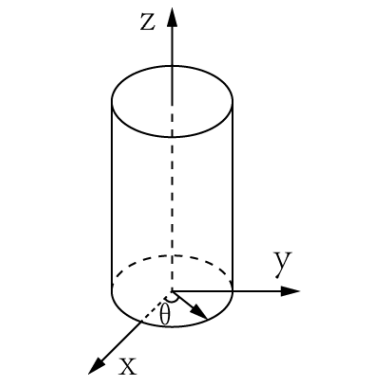
\includegraphics[width=0.3\textwidth]{attachments/fig.illus-1.1.png}
			}		
			\subfloat[The ideal plate thermal model]{\label{fig.illus-1.2}
			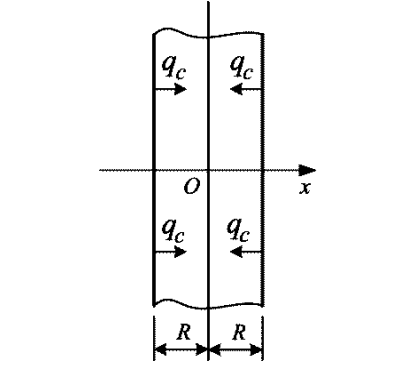
\includegraphics[width=0.3\textwidth]{attachments/fig.illus-1.2.png}
			}
			\caption{\textbf{Illustration of the two ideal thermal models}}
		\end{figure*}

		\begin{figure*}[htbp]
			\centering
			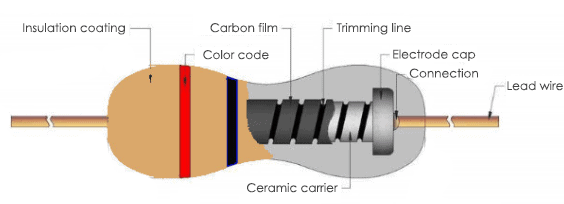
\includegraphics[width=0.4\textwidth]{attachments/fig.illus-1.3.png}
			\caption{\textbf{The structure of a resistor}}
			\label{fig.illus-1.3}
		\end{figure*}

	\subsection{Major instruments and materials}
		\subsubsection{The resistor thermal model}
		Four resistors with different resistance values were connected in series and embedded in the sponge (Fig. \ref{fig.illus-2.1}). 
		Different currents were provided, and the thermocouples were placed in the centers of the surfaces of each resistor. 

		\subsubsection{The plate thermal model}
		As illustrated in Fig. \ref{fig.illus-2.2}, four samples of the same size were placed in a square grid with two heaters embed symmetrically within
		two adjacent samples on both sides, providing stable heat flux. Outside the sample there were insulator which exchanged heat with surroundings following the Newton's cooling law.
		Two themocouples were placed at the central face and the heating face of the model, respectively.
		
		\begin{figure*}[htbp]
			\centering
			\subfloat[The resistor thermal model]{\label{fig.illus-2.1}
			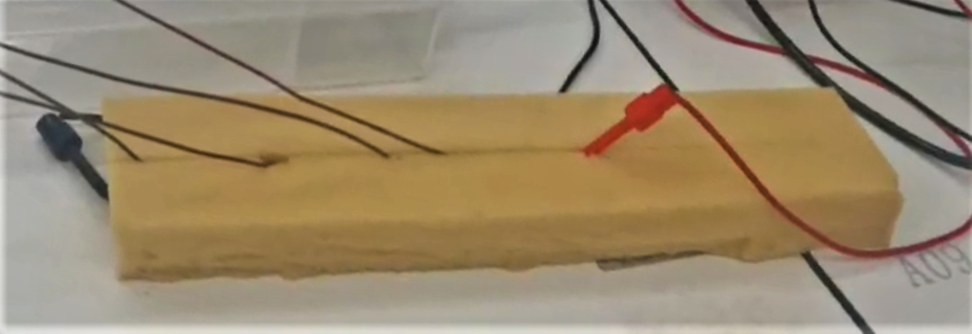
\includegraphics[width=0.4\textwidth]{attachments/fig.illus-2.1.png}
			}		
			\subfloat[The plate thermal model]{\label{fig.illus-2.2}
			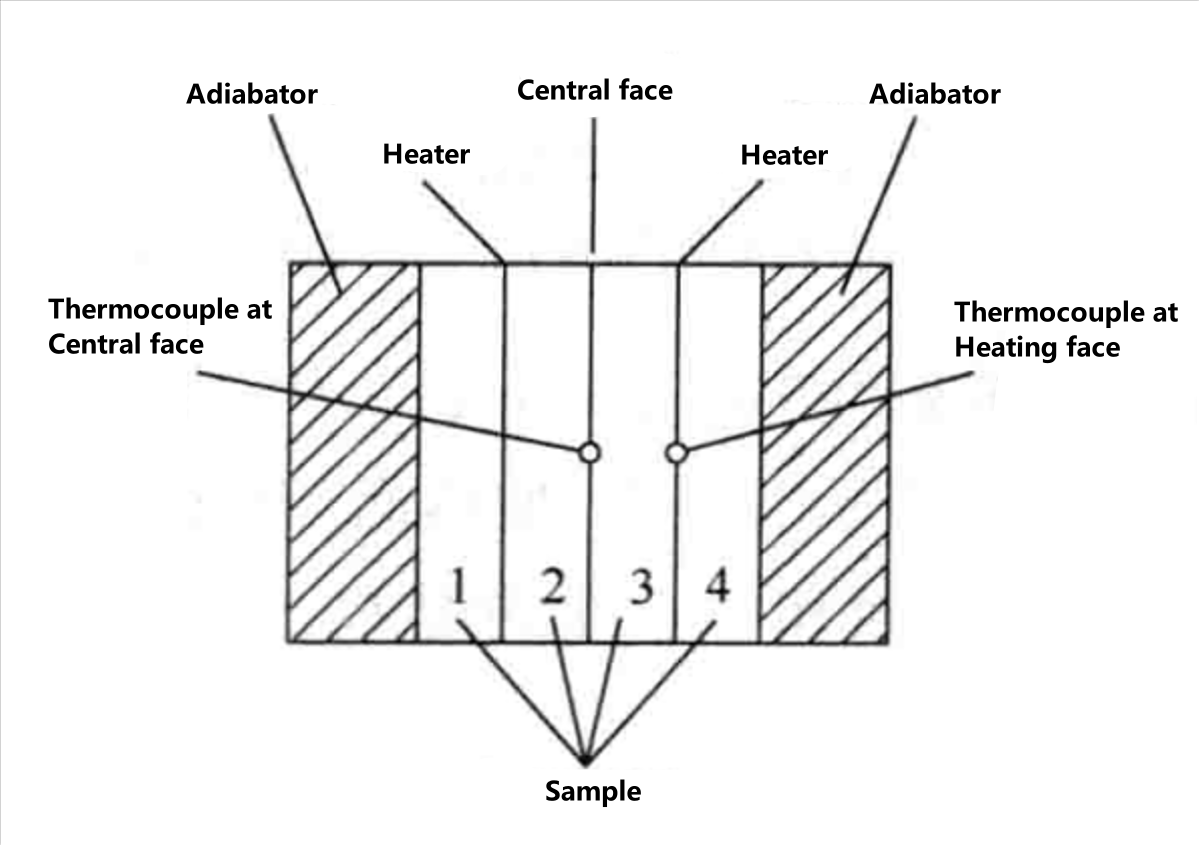
\includegraphics[width=0.4\textwidth]{attachments/fig.illus-2.2.png}
			}
			\caption{\textbf{Illustration of the two thermal models}}
		\end{figure*}

		\subsubsection{CompactDAQ multichannel data acquisition system and LabVIEW virtual instrument}
		\paragraph{A. CompactDAQ}~
		\newline 
		In this research we use CompactDAQ platform ($NI\ CDAQ\ NI\ 9171$) integrated with high density thermocouples module ($NI \ 9211$) to collect the temperature measurements data.

		CompactDAQ is a data acquisition platform built by National Instruments that includes a broad set of compatible hardware and software. 
		CompactDAQ integrates hardware for data I/O with LabVIEW software to enable researchers to collect, process, and analyze sensor data. It can be directly connected to various kinds of sensors and manage multichannel data c tasks simultaneously.

		The high density thermocouple module ($NI \ 9211$) is a multichannel temperature measuring instrument that can link to up to four thermocouples (Fig. \ref{fig.illus-3.1} and Fig. \ref{fig.illus-3.2}). 
		The data collected in each acquisition channel will be preprocessed and transformed into digital signals by a 24-bit ADC (Fig. \ref{fig.illus-3.3}). 

		\begin{figure*}[htbp]
			\centering
			\subfloat[Schematic of the pins]{\label{fig.illus-3.1}
			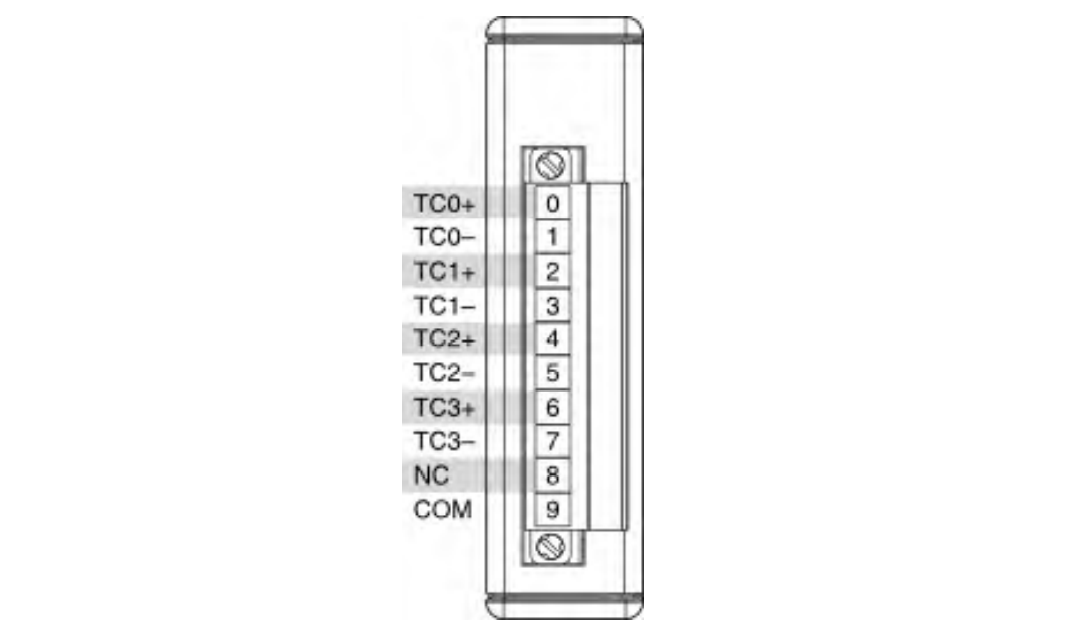
\includegraphics[width=0.3\textwidth]{attachments/fig.illus-3.1.png}
			}		
			\subfloat[Schematic of connection]{\label{fig.illus-3.2}
			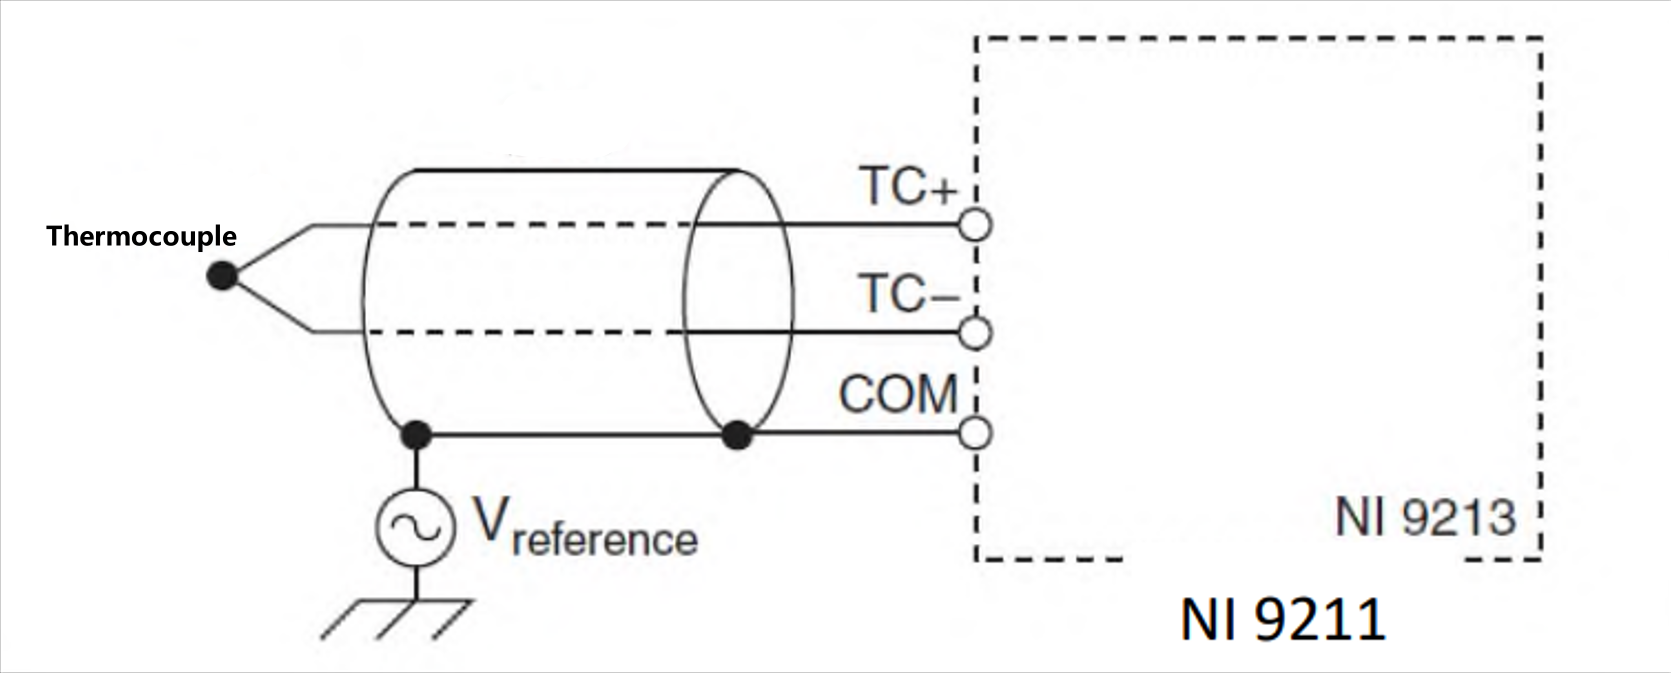
\includegraphics[width=0.3\textwidth]{attachments/fig.illus-3.2.png}
			}
			\subfloat[Schematic of the signal processing]{\label{fig.illus-3.3}
			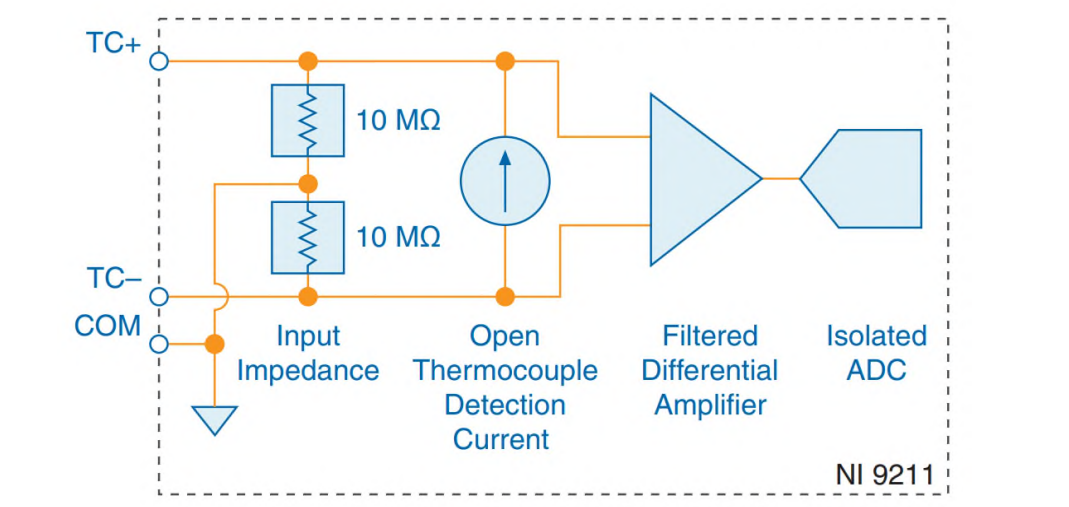
\includegraphics[width=0.3\textwidth]{attachments/fig.illus-3.3.png}
			}
			\caption{\textbf{High density thermocouples module ($NI \ 9211$)}}
		\end{figure*}

		\paragraph{B. LabVIEW virtual instrument}~
		\newline 
		Data collected from CompactDAQ platform can be directly imported and processed by the LabVIEW software. 
		In this research, we programmed and built a virtual thermometer in the LabVIEW platform and used it to integrate the temperature measurements. 
		The program and panel interface are illustrated in Fig. \ref{fig.illus-4.1} and Fig. \ref{fig.illus-4.2}, respectively.

		\begin{figure*}[htbp]
			\centering
			\subfloat[The program interface]{\label{fig.illus-4.1}
			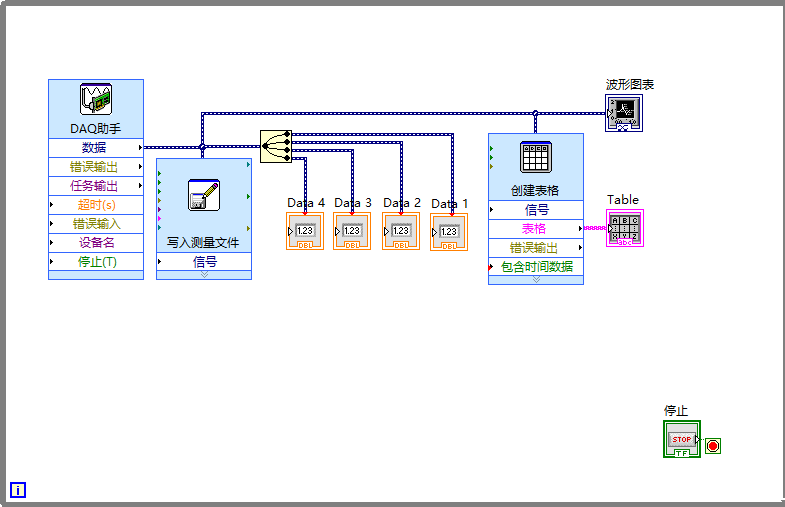
\includegraphics[width=0.45\textwidth]{attachments/fig.illus-4.1.png}
			}		
			\subfloat[The panel interface]{\label{fig.illus-4.2}
			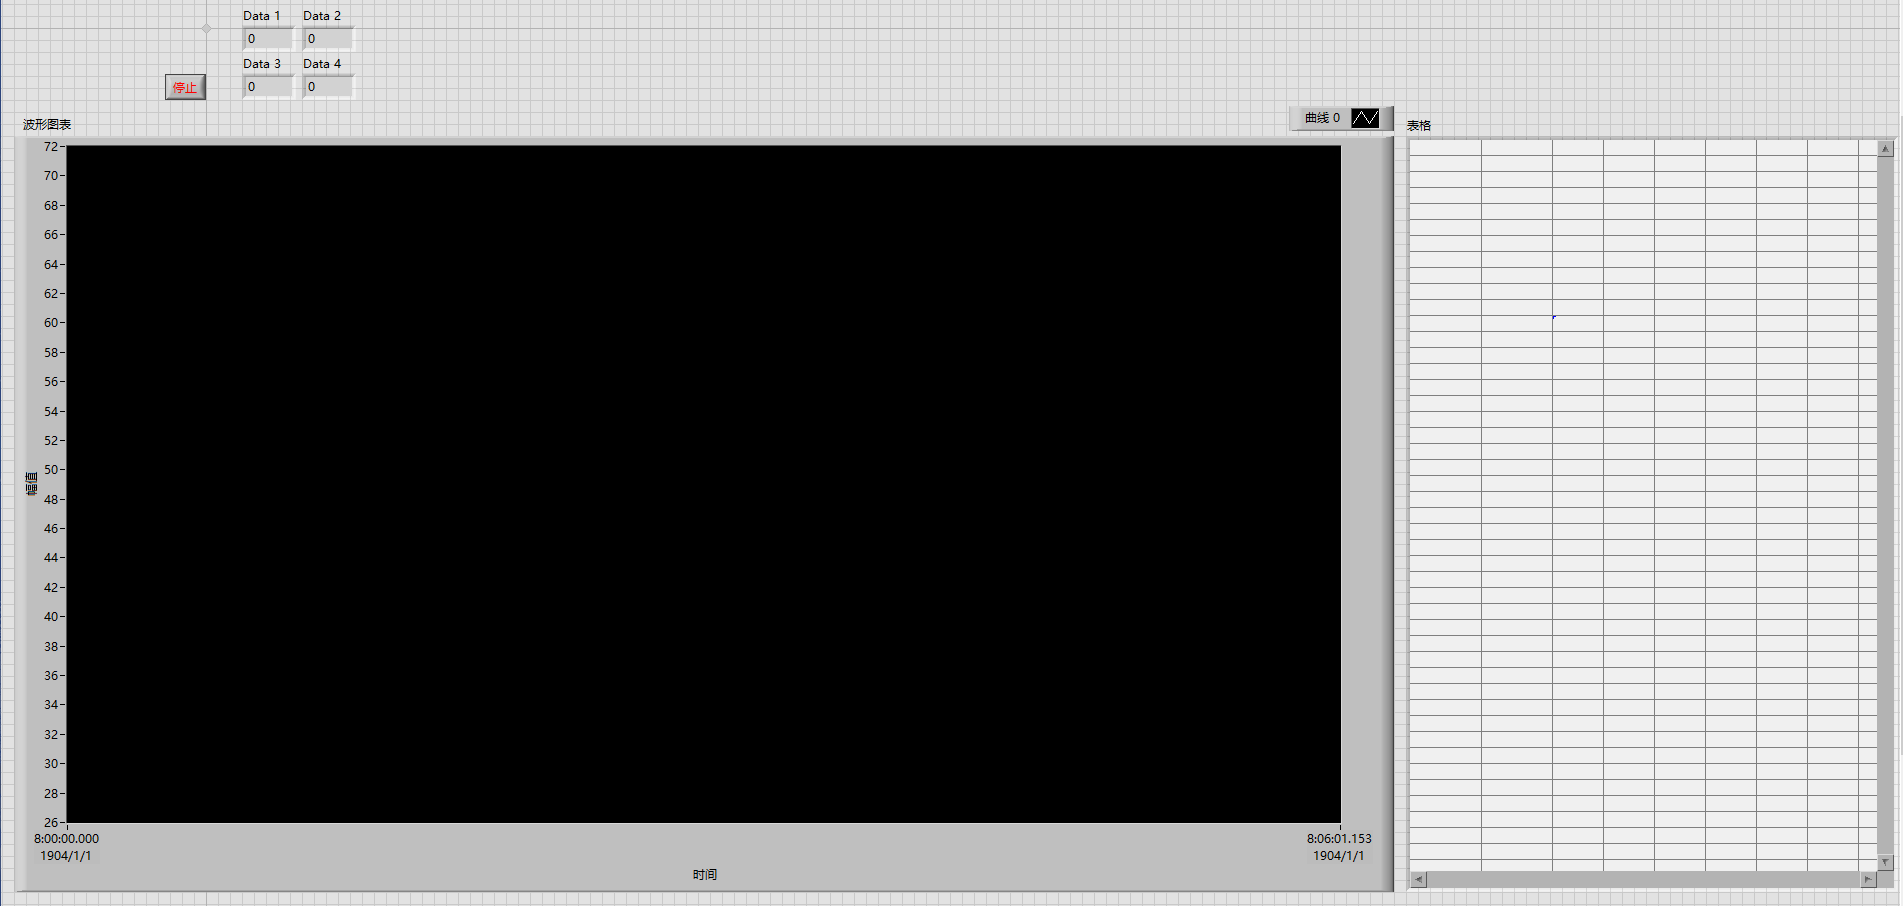
\includegraphics[width=0.45\textwidth]{attachments/fig.illus-4.2.png}
			}
			\caption{\textbf{Virtual thermometer}}
		\end{figure*}

		\subsubsection{Multiphysics simulation platform COMSOL}
		COMSOL Multiphysics is a cross-platform finite element analysis solver and multiphysics simulation software. 
		It allows conventional physics-based user interfaces and coupled systems of partial differential equations. 
		COMSOL provides an IDE and unified workflow for electrical, mechanical, fluid, acoustic, and chemical applications.

		In this research, the thermal models of resistor and plate were built and simulated on COMSOL platform, and the distribution of the temperature fields and their evolution over time were obtained. 

	\subsection{Method}
	For the resistor thermal model, different currents were provided to the series resistors and changes of surface temperature of every resistor over time were collected. 
	After equilibrium was reached, the current was removed, and the cooling curves were obtained. The relationship between equilibrium temperature and heating power were also investigated.

	For the thermal model of the plate, with continuous injection of stable heat into the system, after the system reached the quasi-stable stage, 
	the temperature difference between the surface and the center face $\Delta t$ and the rate of temperature changes in the center face $\frac{dt}{d\tau}$ were calculated.

	For both models, the real-world experiments and COMSOL simulation experiments were conducted, and their results were compared.

%%end-------------------Method-----------------------%%

%%begin-------------------Result-----------------------%%
\section{Result}
	\subsection{The resistor thermal model}
	\paragraph{A. Real-world experiment}~
	\newline 
	\indent
	Four resistors with different resistance values were connected in series and embedded in the sponge. 
	With different currents provided, the heating curves and the following cooling curves (Fig. \ref{fig.1.1.1}) were obtained from the thermocouples placed on each resistor.
	The results show that for the resistor heating model, as the current starts to flow through the resistor, the surface temperature began to increase.
	After a rapid climbing of the temperature, the thermal system gradually reached an equilibrium, and the temperature finally become stable.
	If the current was removed, the temperature began to drop and finally reached room temperature.

	The equilibrium temperatures of each resistor were defined as the maximum temperature before the cooling process, 
	and their correlation with the heating power is shown in Fig. \ref{fig.1.1.2}.
	Results show that the equilibrium temperature was directly proportional to the resist value.

	Simultaneously, the simulation experiments were conducted.
	\begin{figure*}[htbp]
		\centering
		\subfloat[$I=0.020A$]{\label{fig.1.1.1.1}
		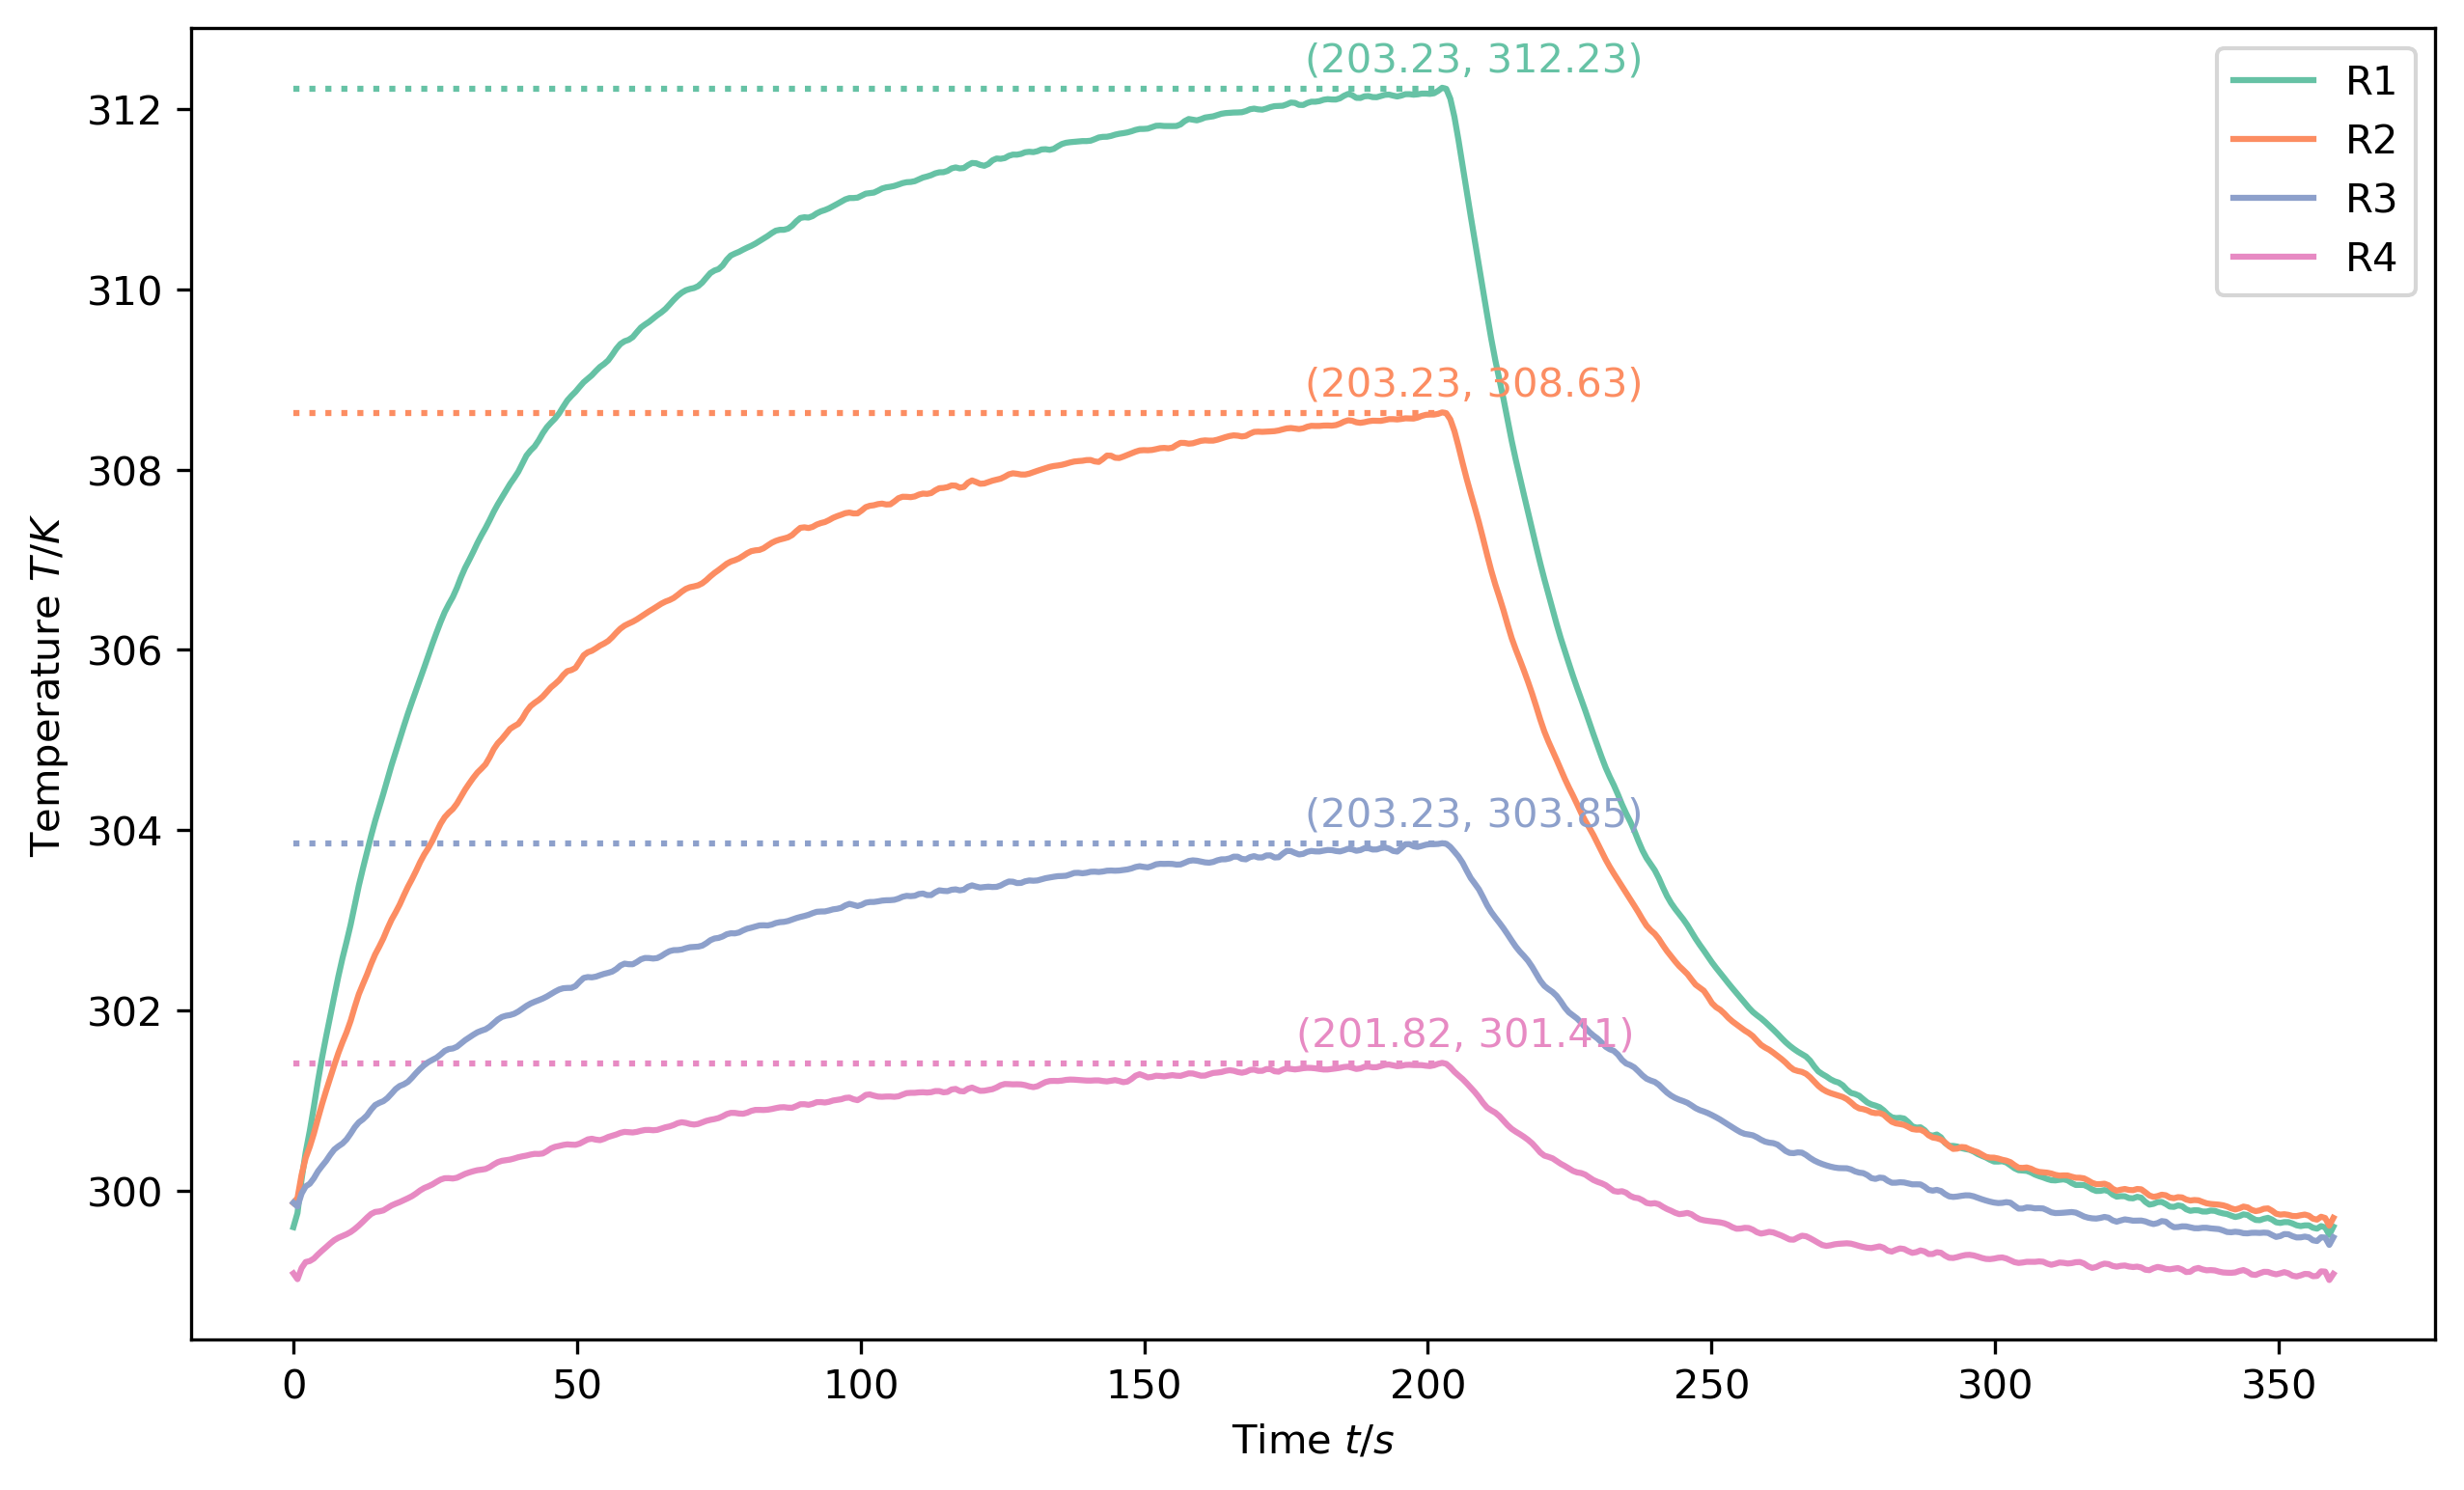
\includegraphics[width=0.3\textwidth]{attachments/fig.1.1.1.1.png}
		}		
		\subfloat[$I=0.025A$]{\label{fig.1.1.1.2}
		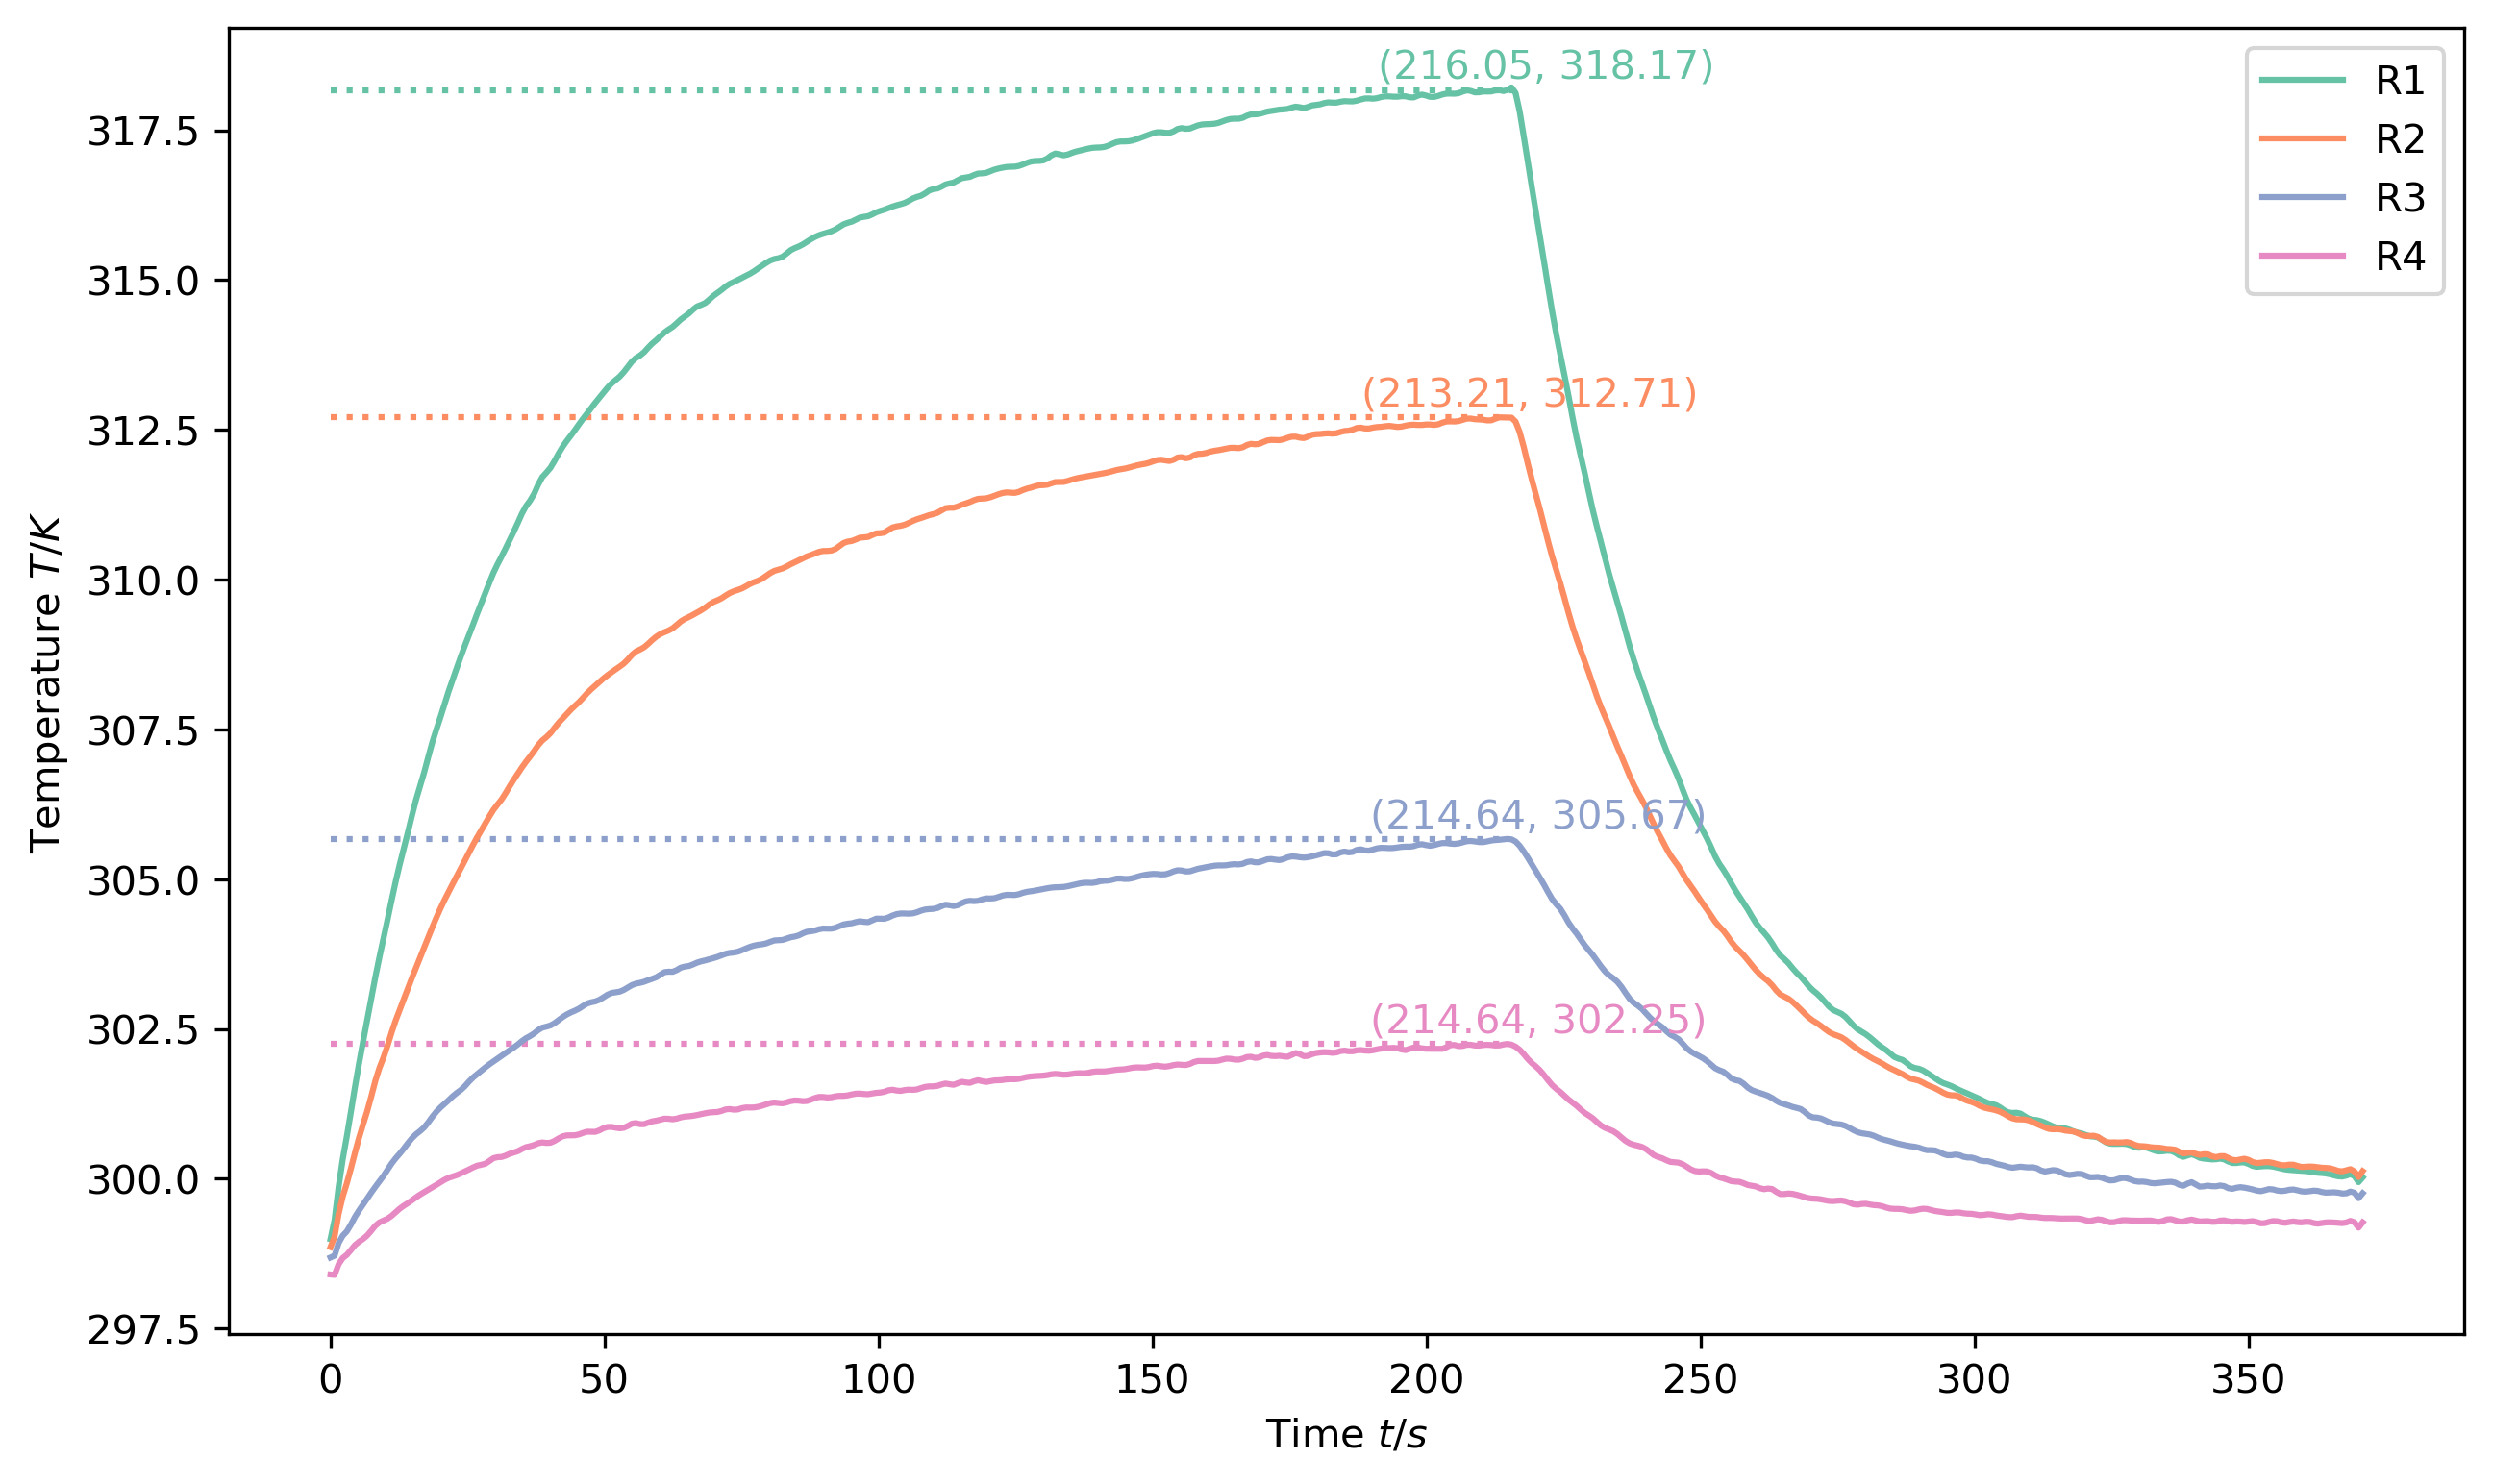
\includegraphics[width=0.3\textwidth]{attachments/fig.1.1.1.2.png}
		}

		\subfloat[$I=0.030A$]{\label{fig.1.1.1.3}
		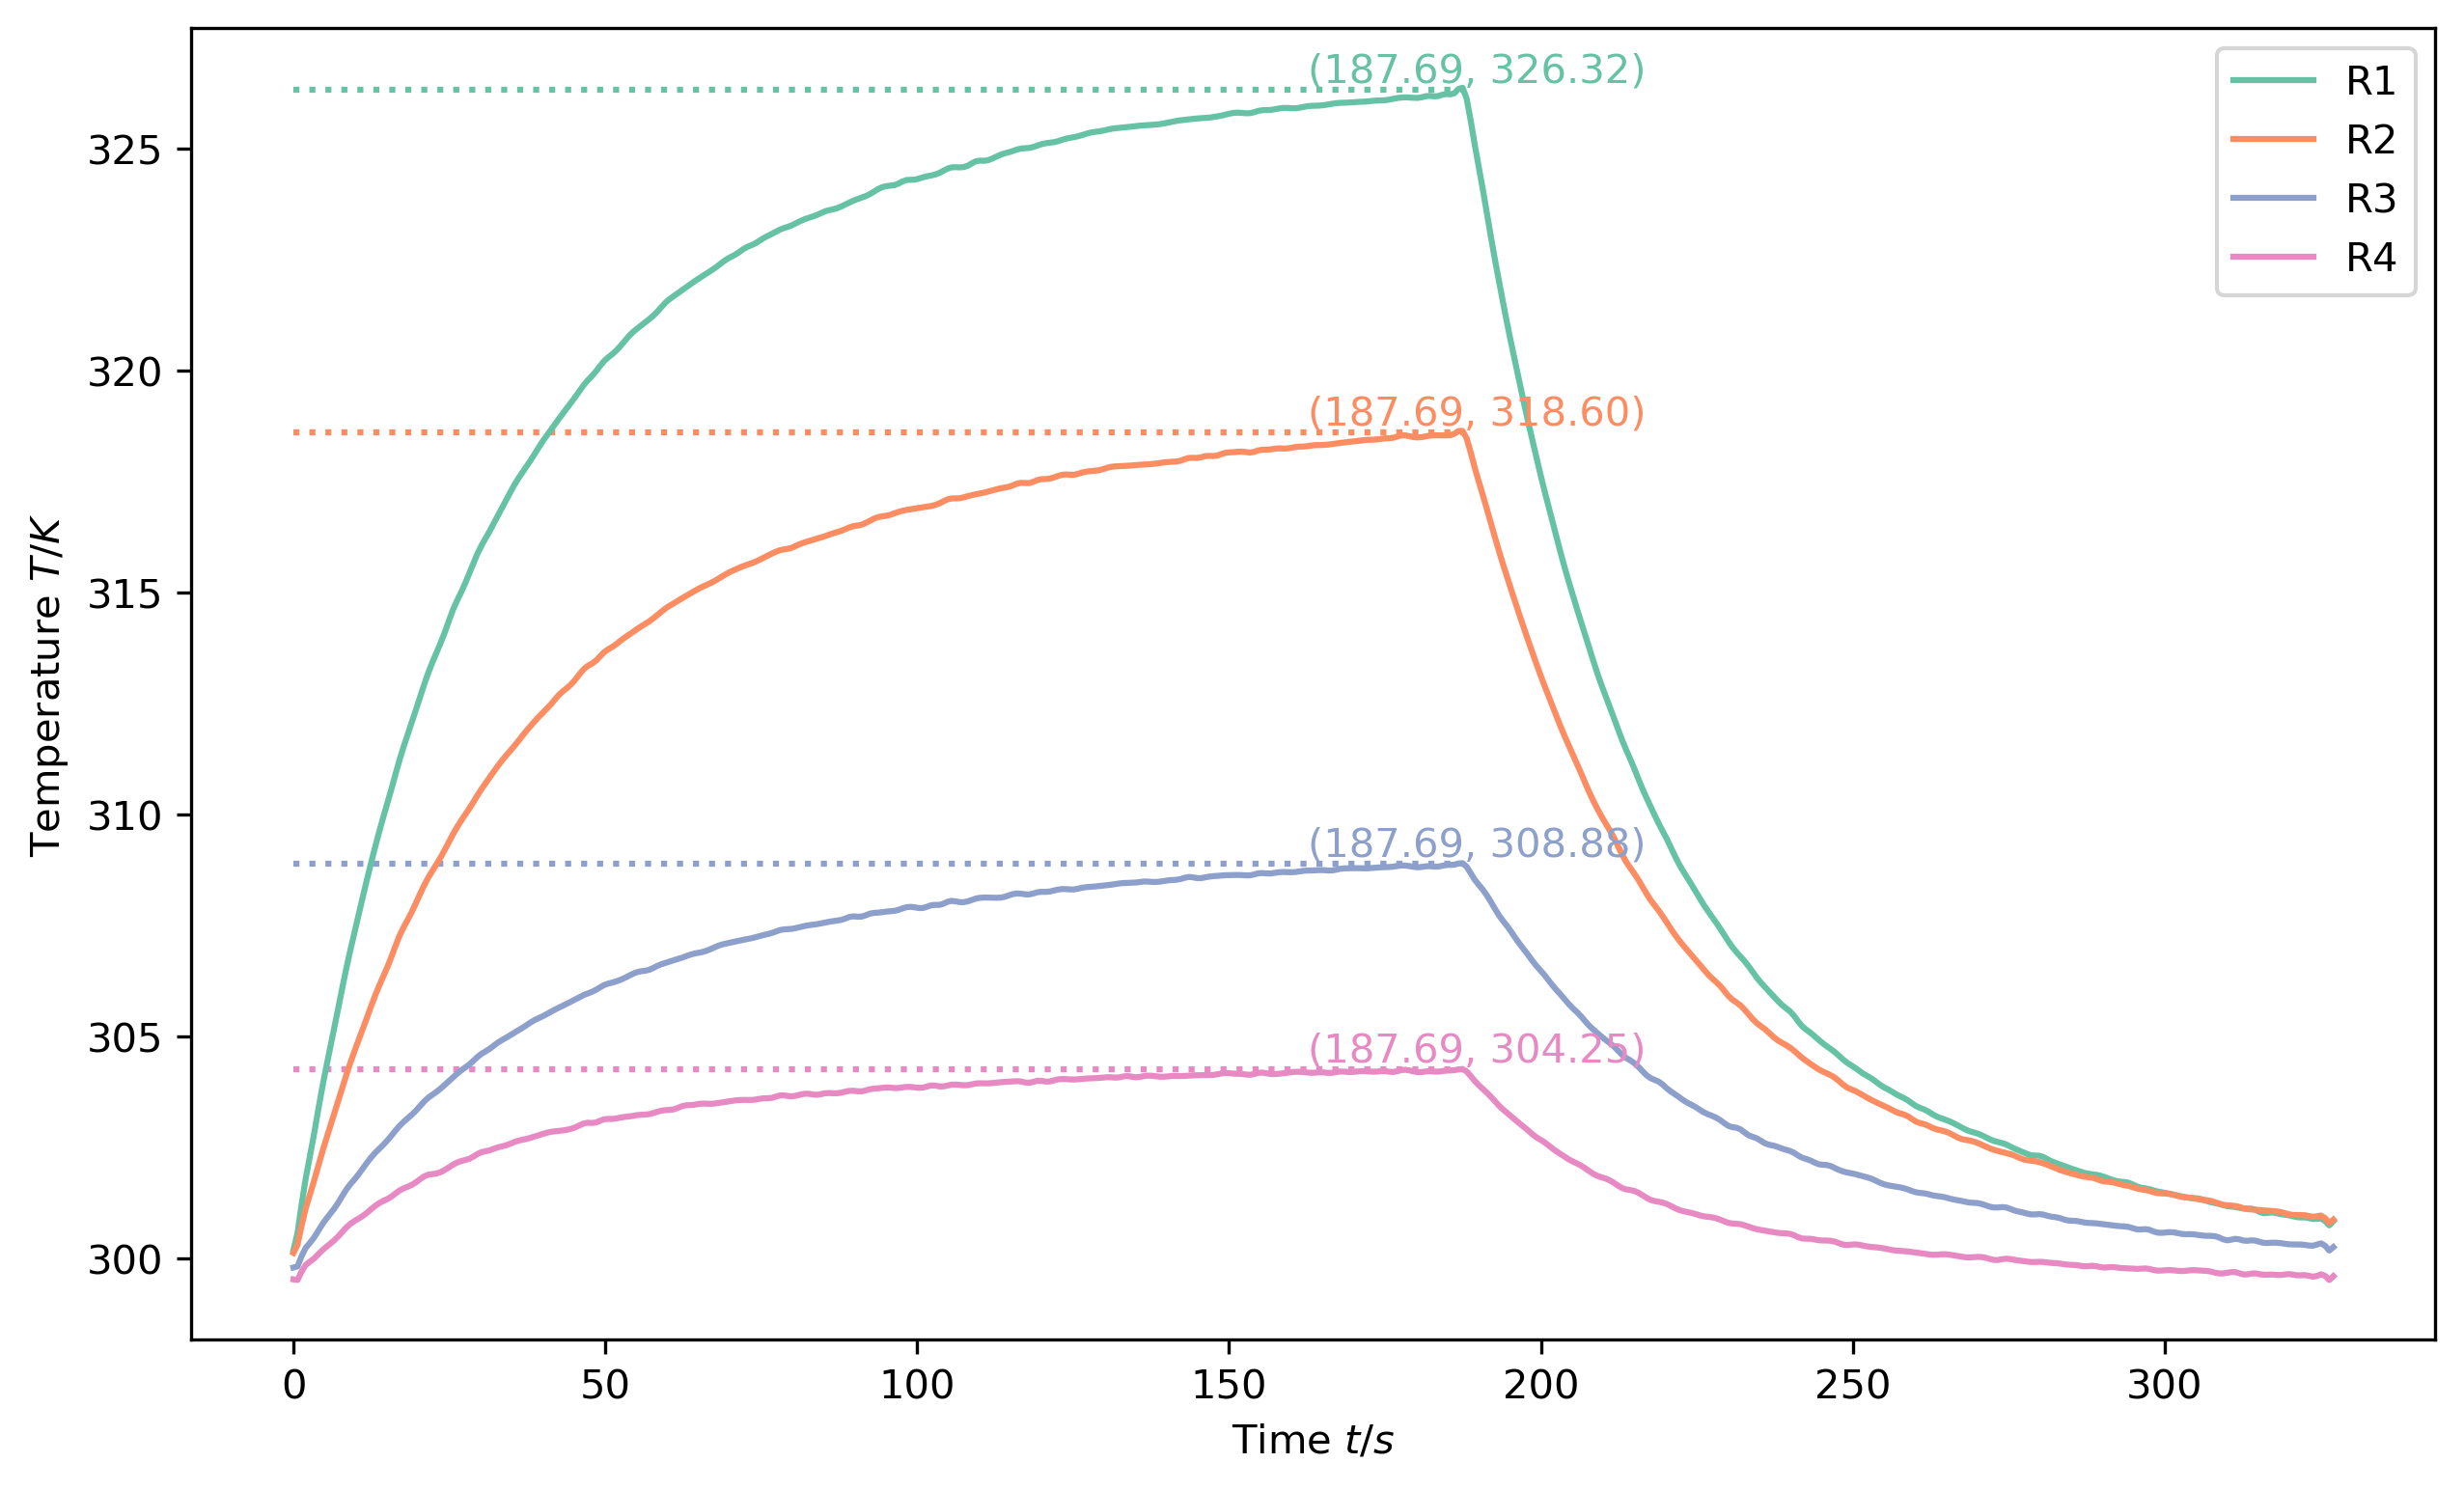
\includegraphics[width=0.3\textwidth]{attachments/fig.1.1.1.3.png}
		}
		\subfloat[$I=0.035A$]{\label{fig.1.1.1.4}
		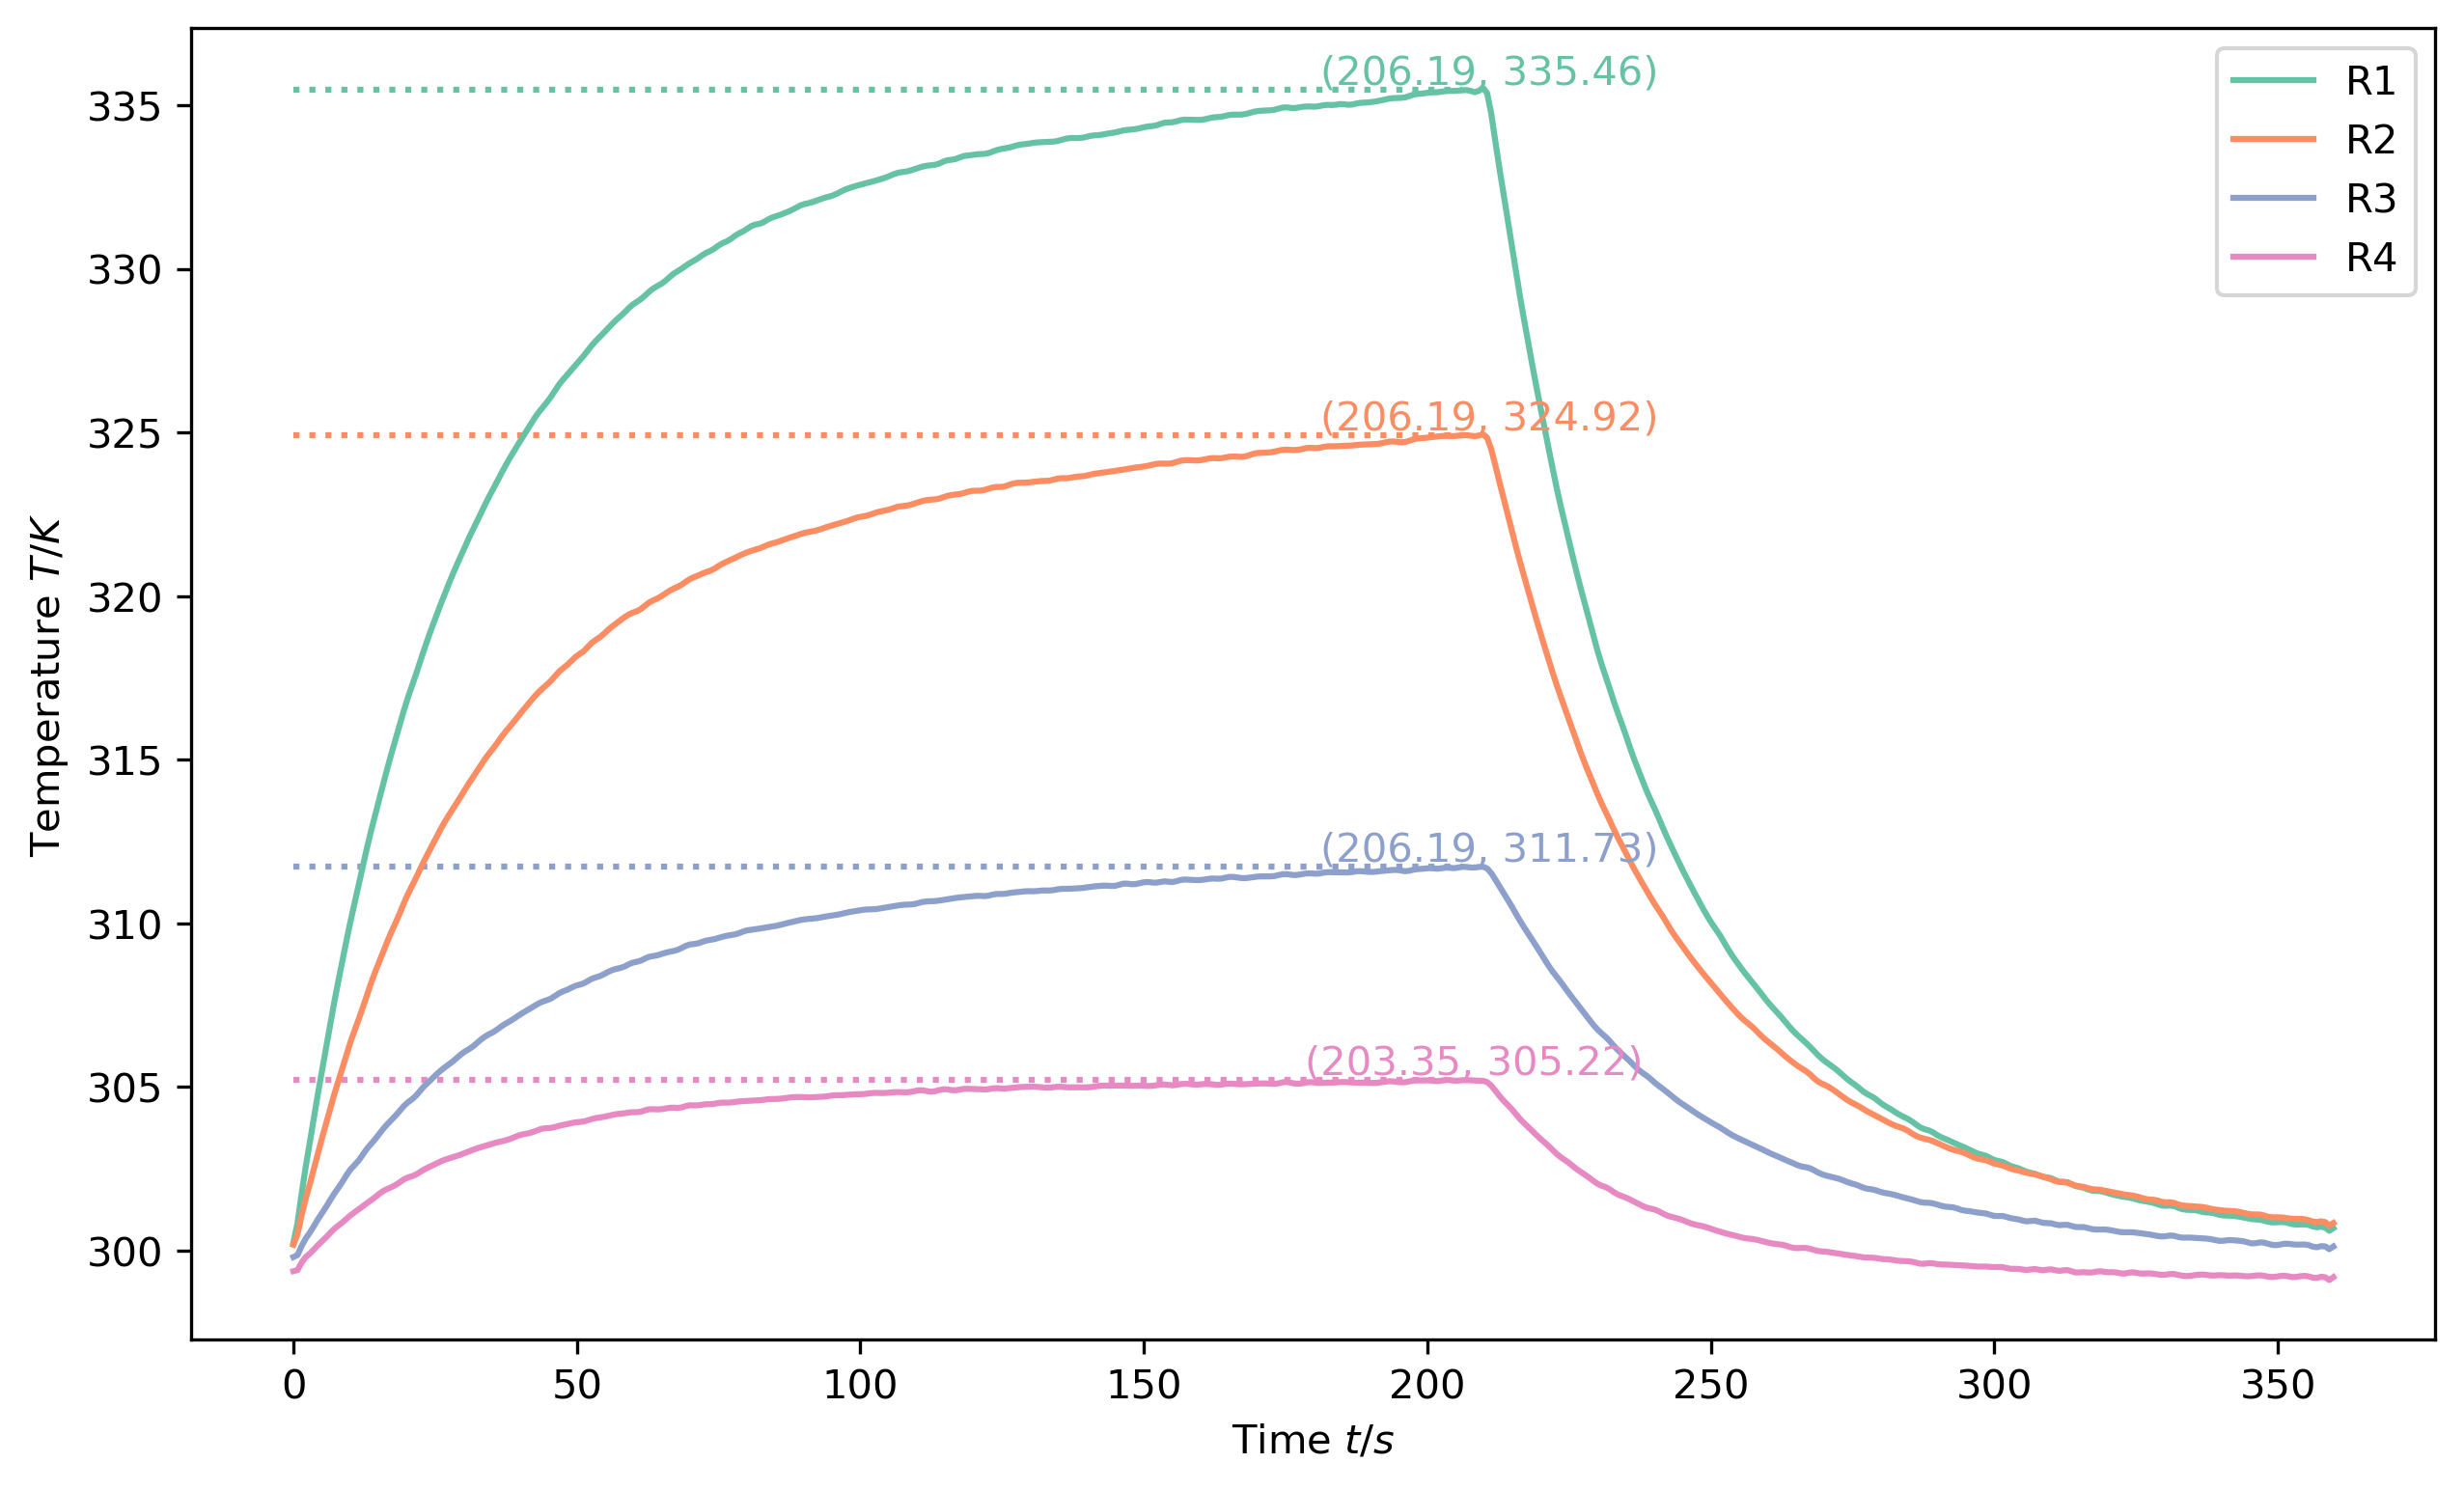
\includegraphics[width=0.3\textwidth]{attachments/fig.1.1.1.4.png}
		}
		\subfloat[$I=0.040A$]{\label{fig.1.1.1.5}
		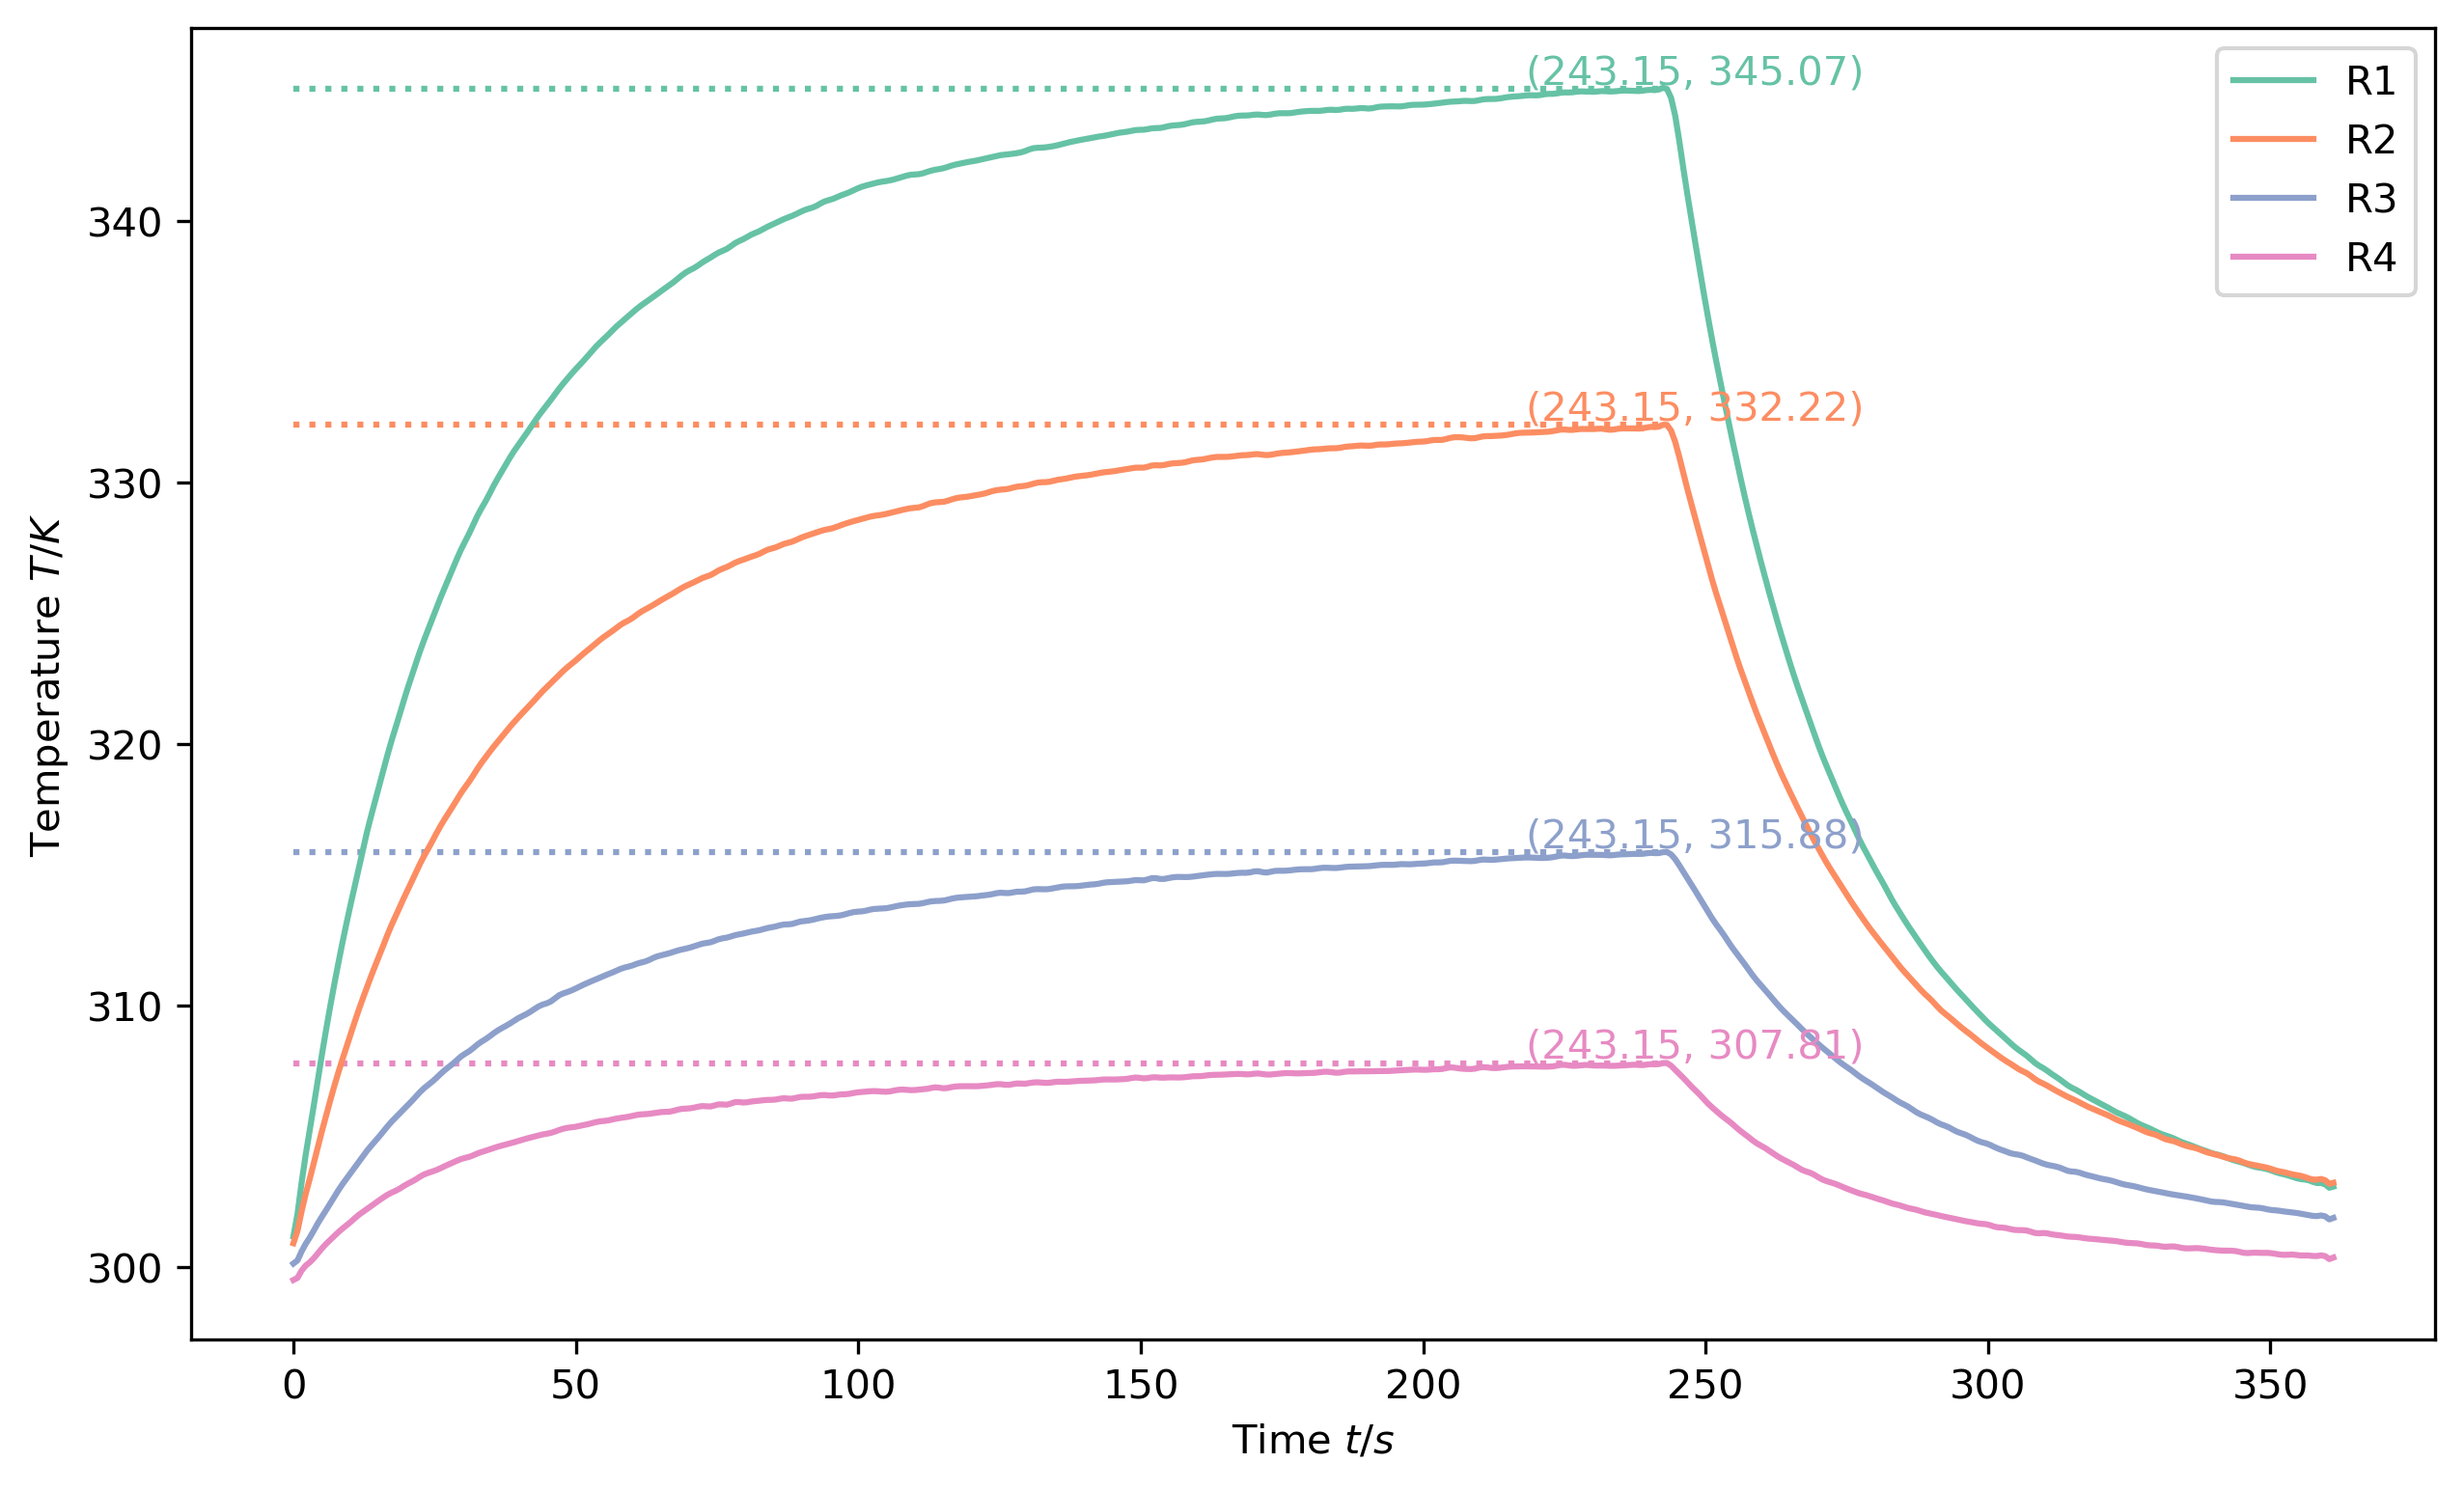
\includegraphics[width=0.3\textwidth]{attachments/fig.1.1.1.5.png}
		}
		\caption{\textbf{Heating and cooling curves of the series resistors under different currents, real-world experiments}}
		\label{fig.1.1.1}
	\end{figure*}

	\begin{figure*}[htbp]
		\centering
		\subfloat[$R_1 = 100.00 \Omega$]{\label{fig.1.1.2.1}
		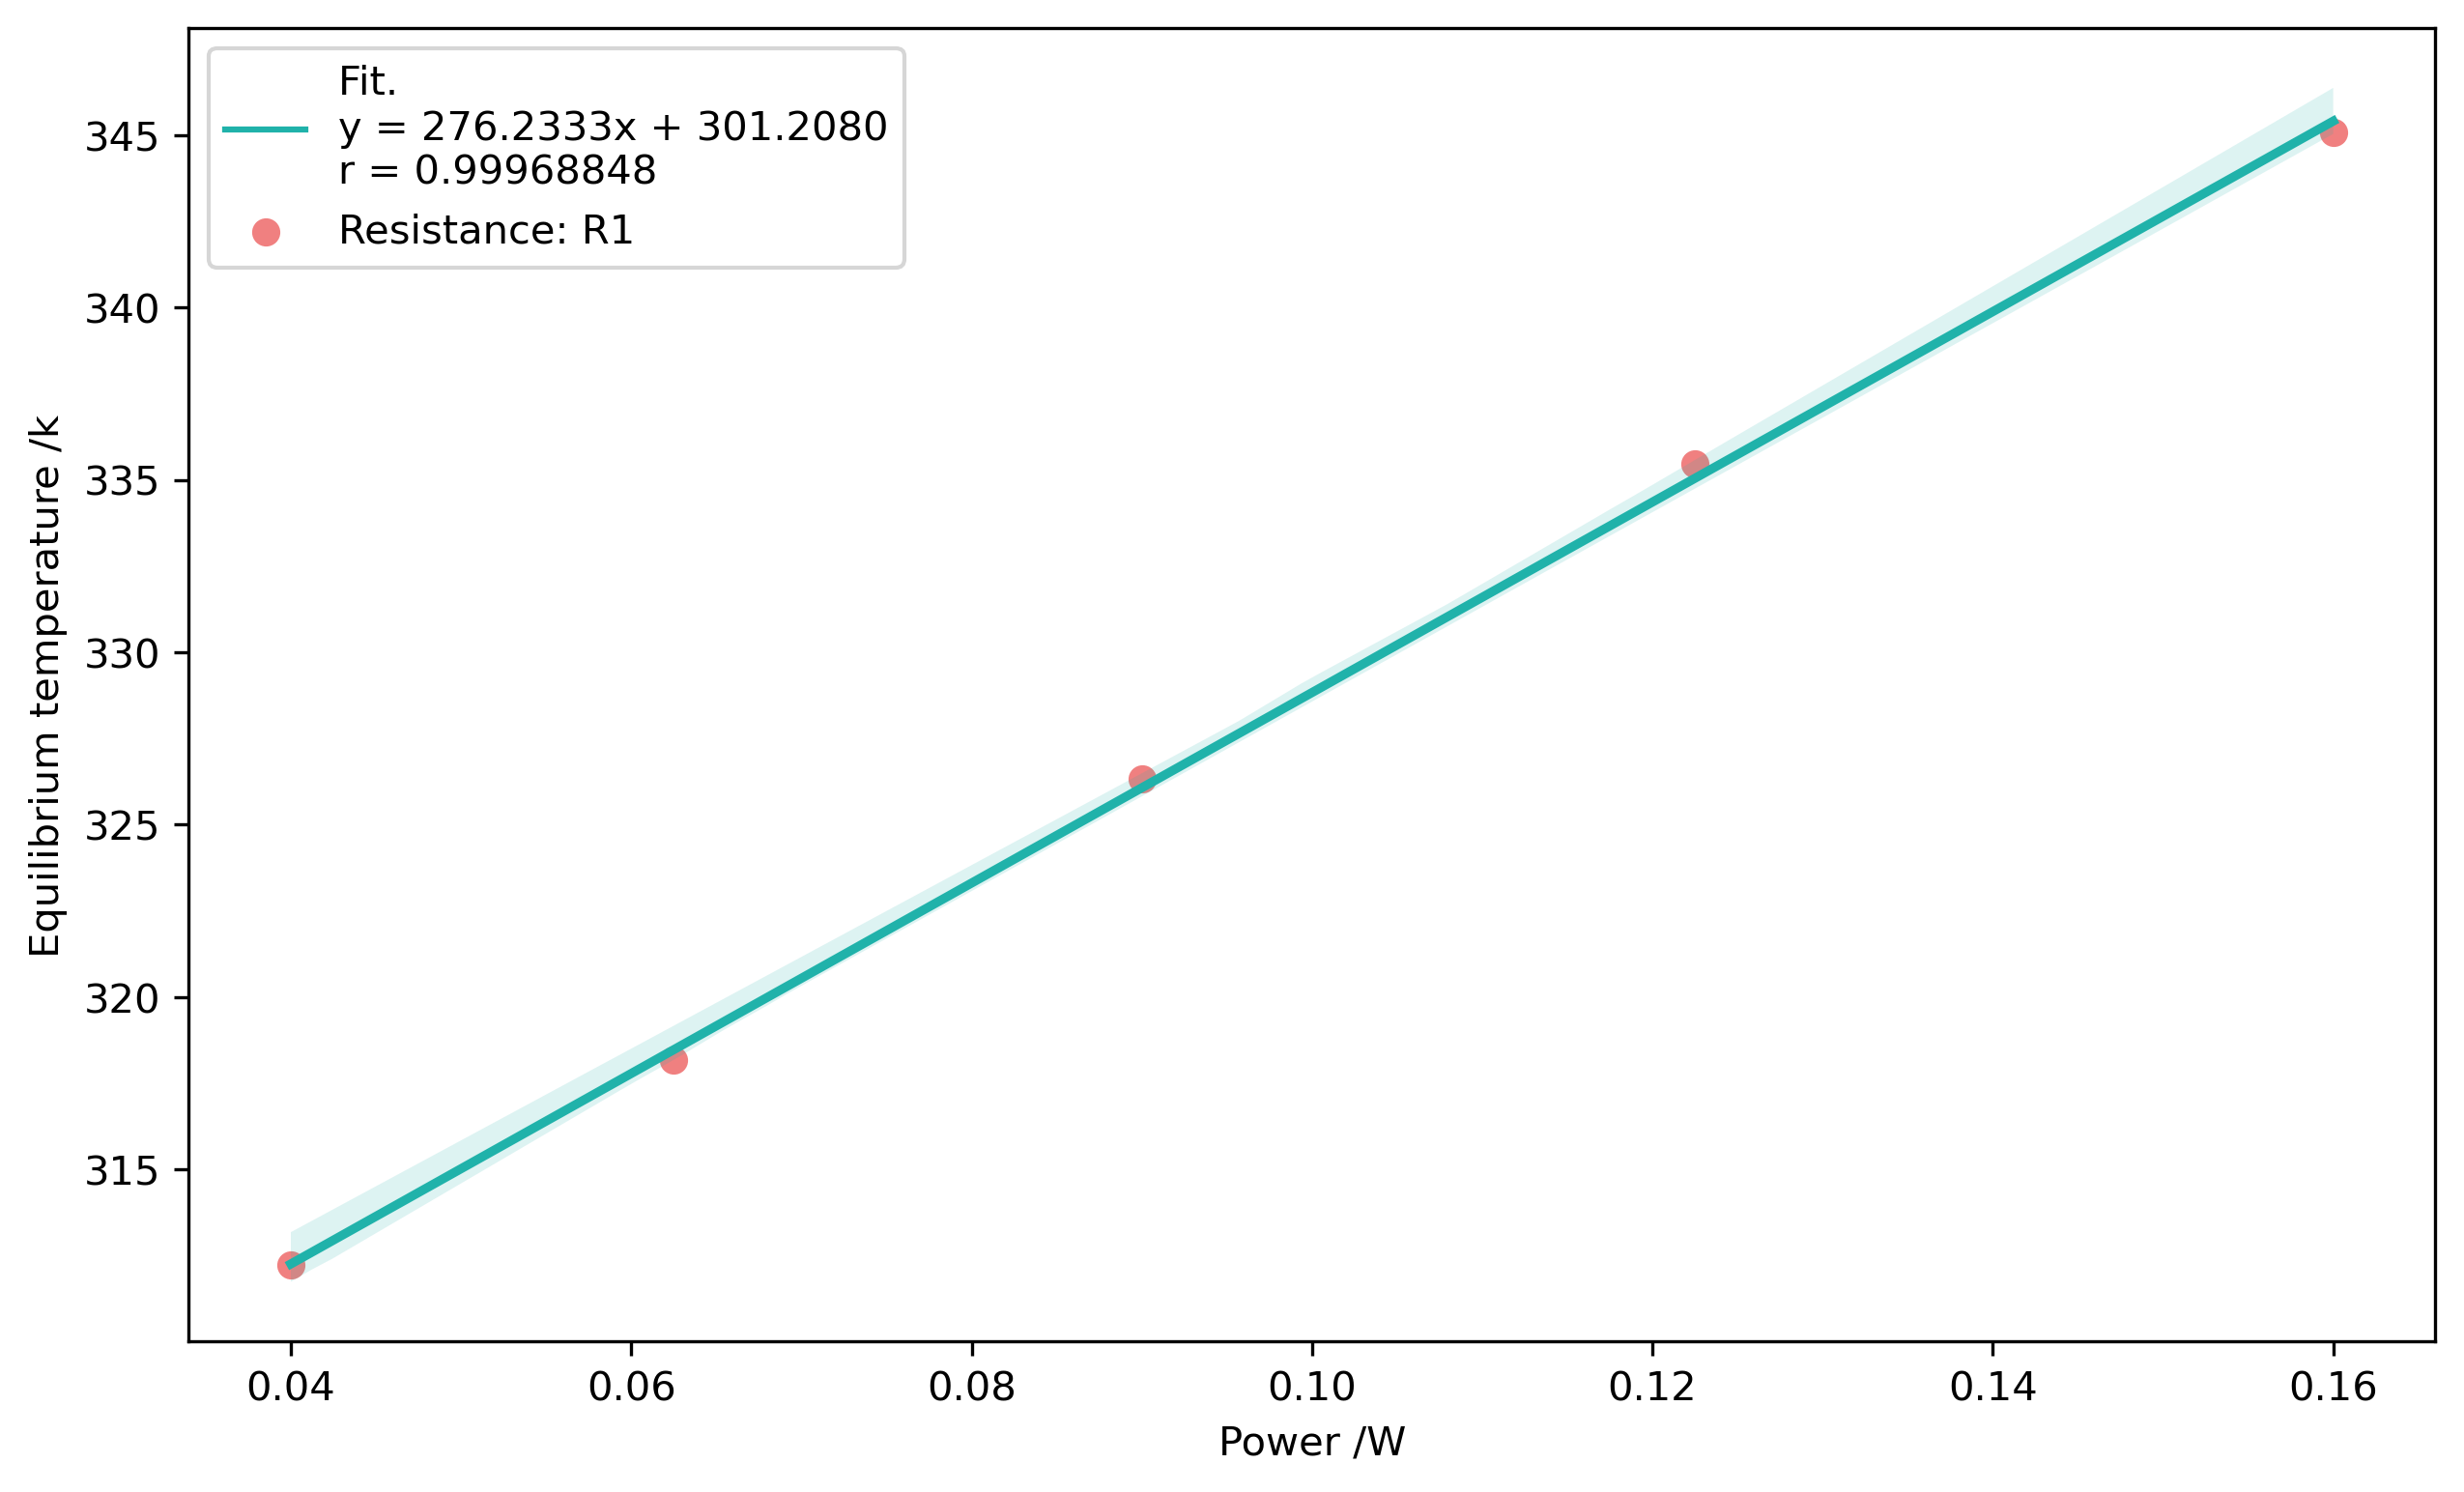
\includegraphics[width=0.3\textwidth]{attachments/fig.1.1.2.1.png}
		}		
		\subfloat[$R_2 = 81.588 \Omega$]{\label{fig.1.1.2.2}
		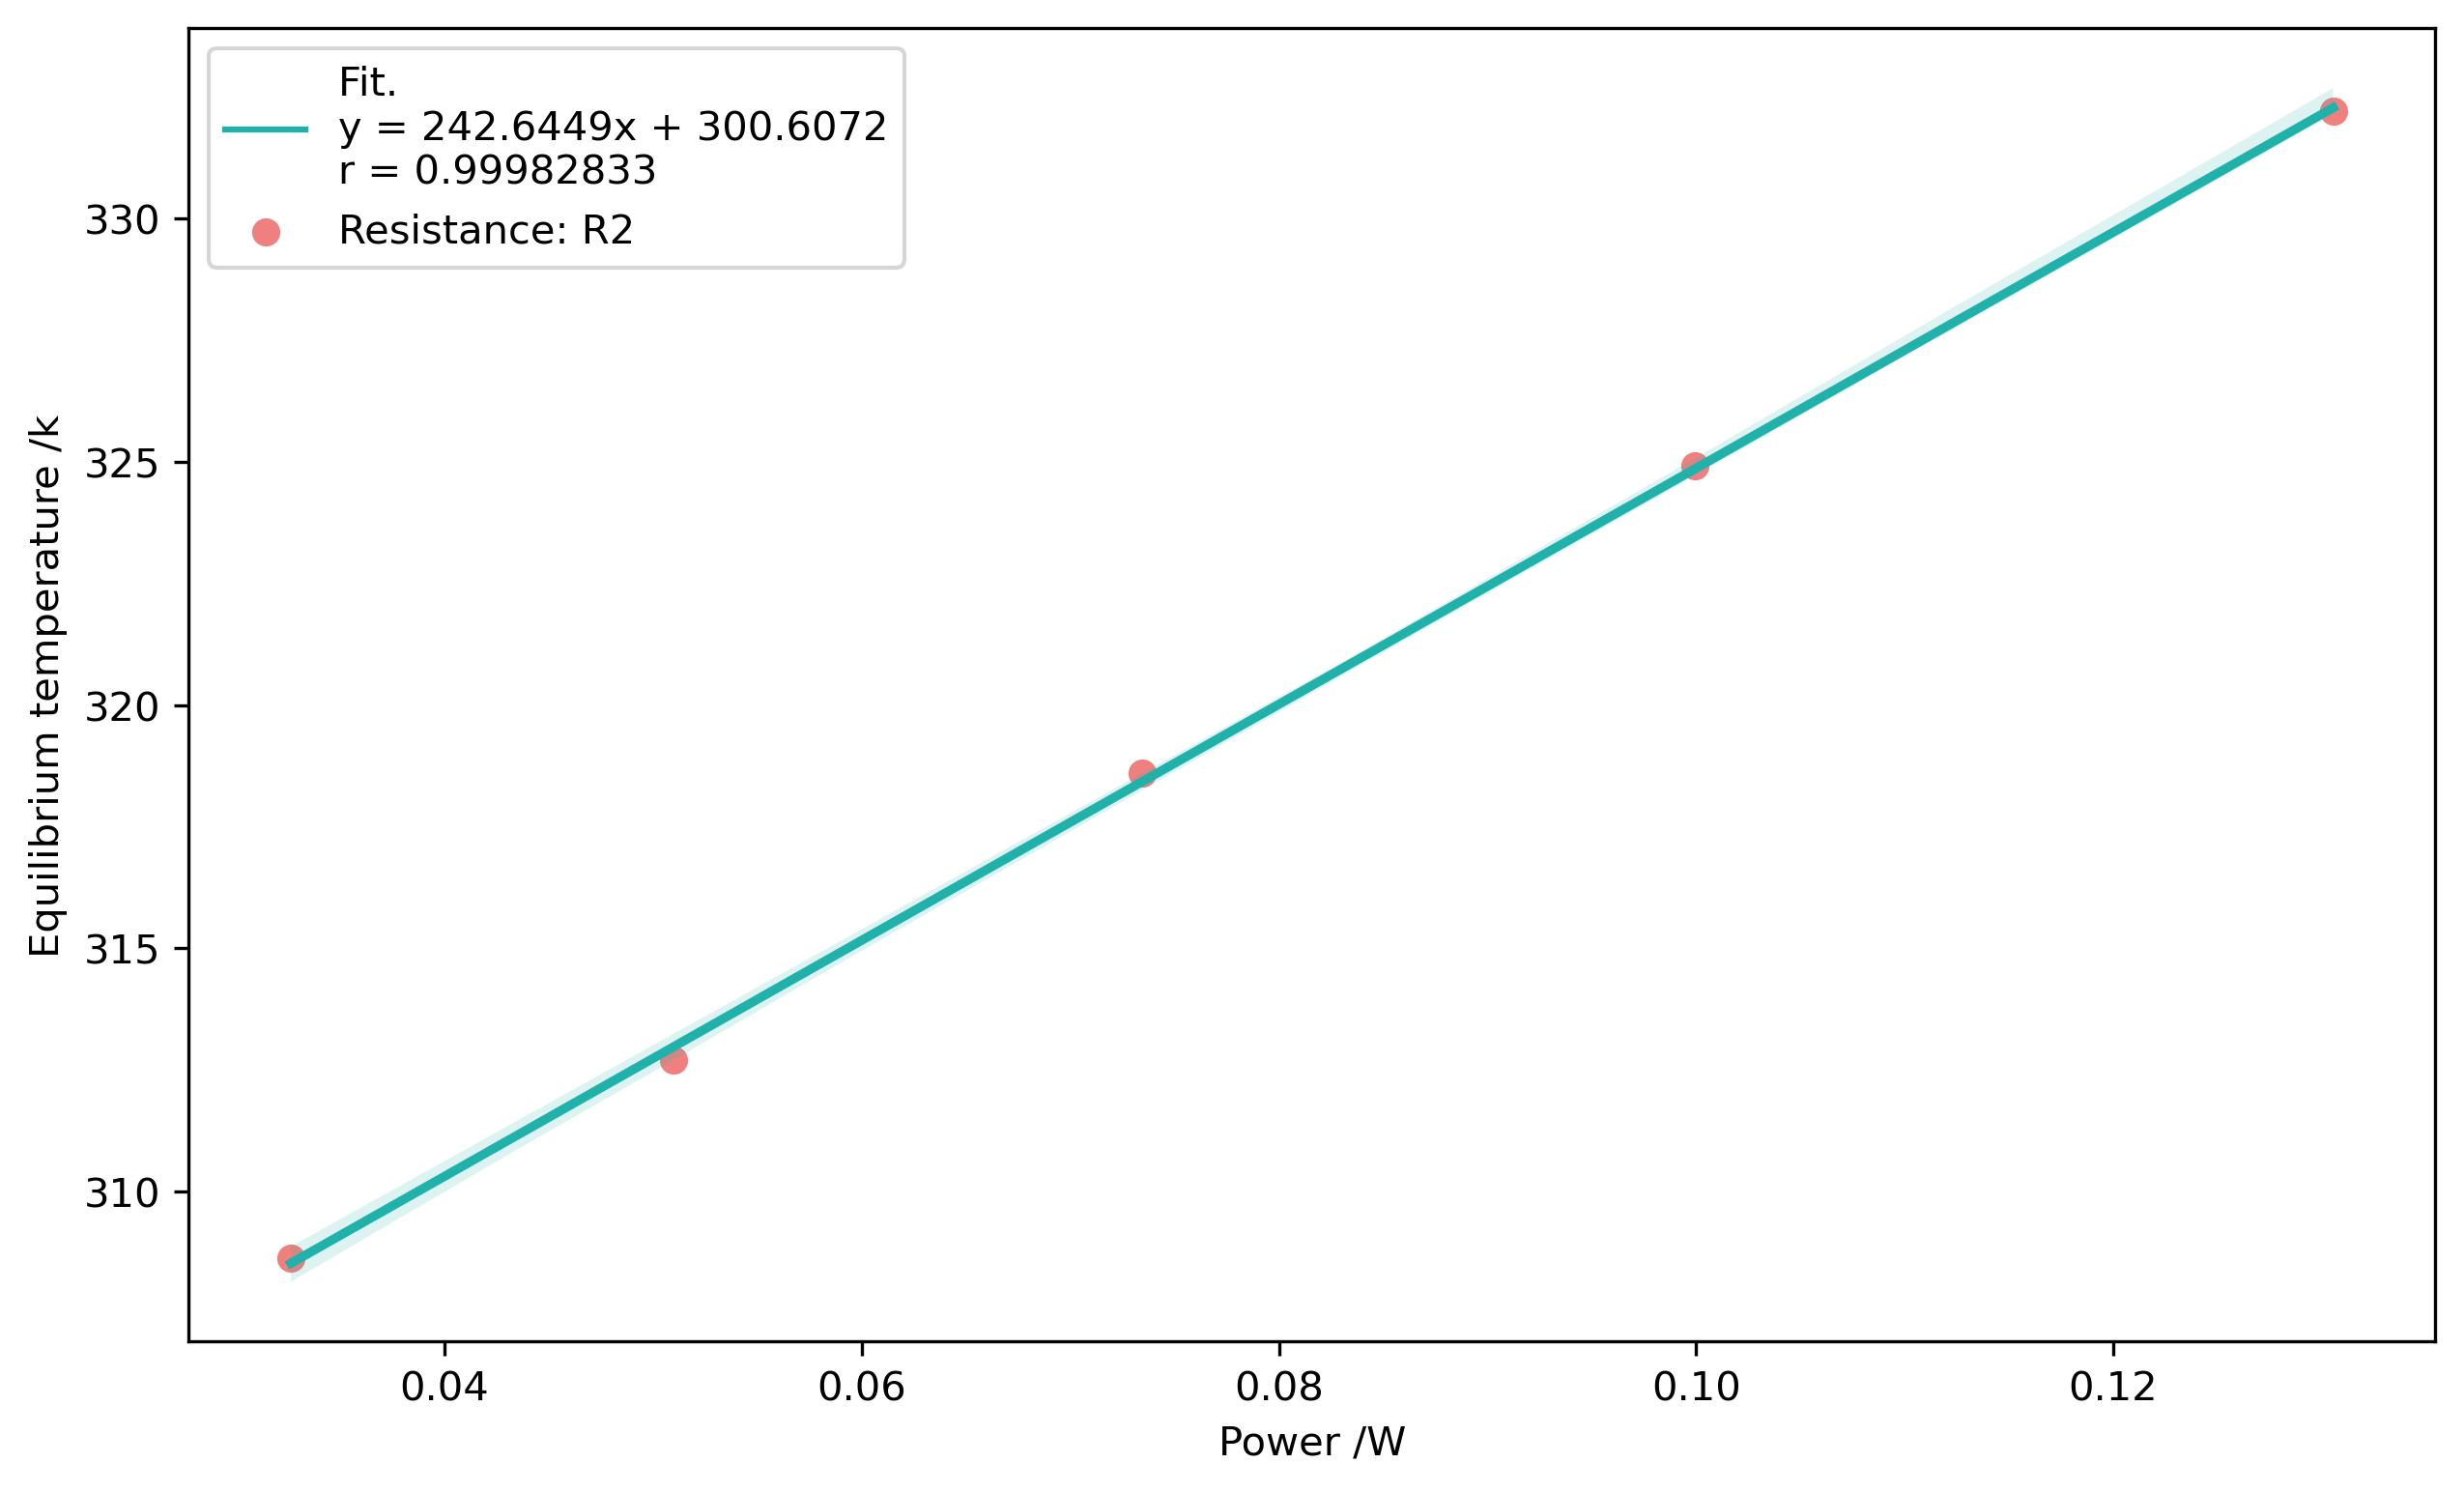
\includegraphics[width=0.3\textwidth]{attachments/fig.1.1.2.2.png}
		}

		\subfloat[$R_3 = 42.902 \Omega$]{\label{fig.1.1.2.3}
		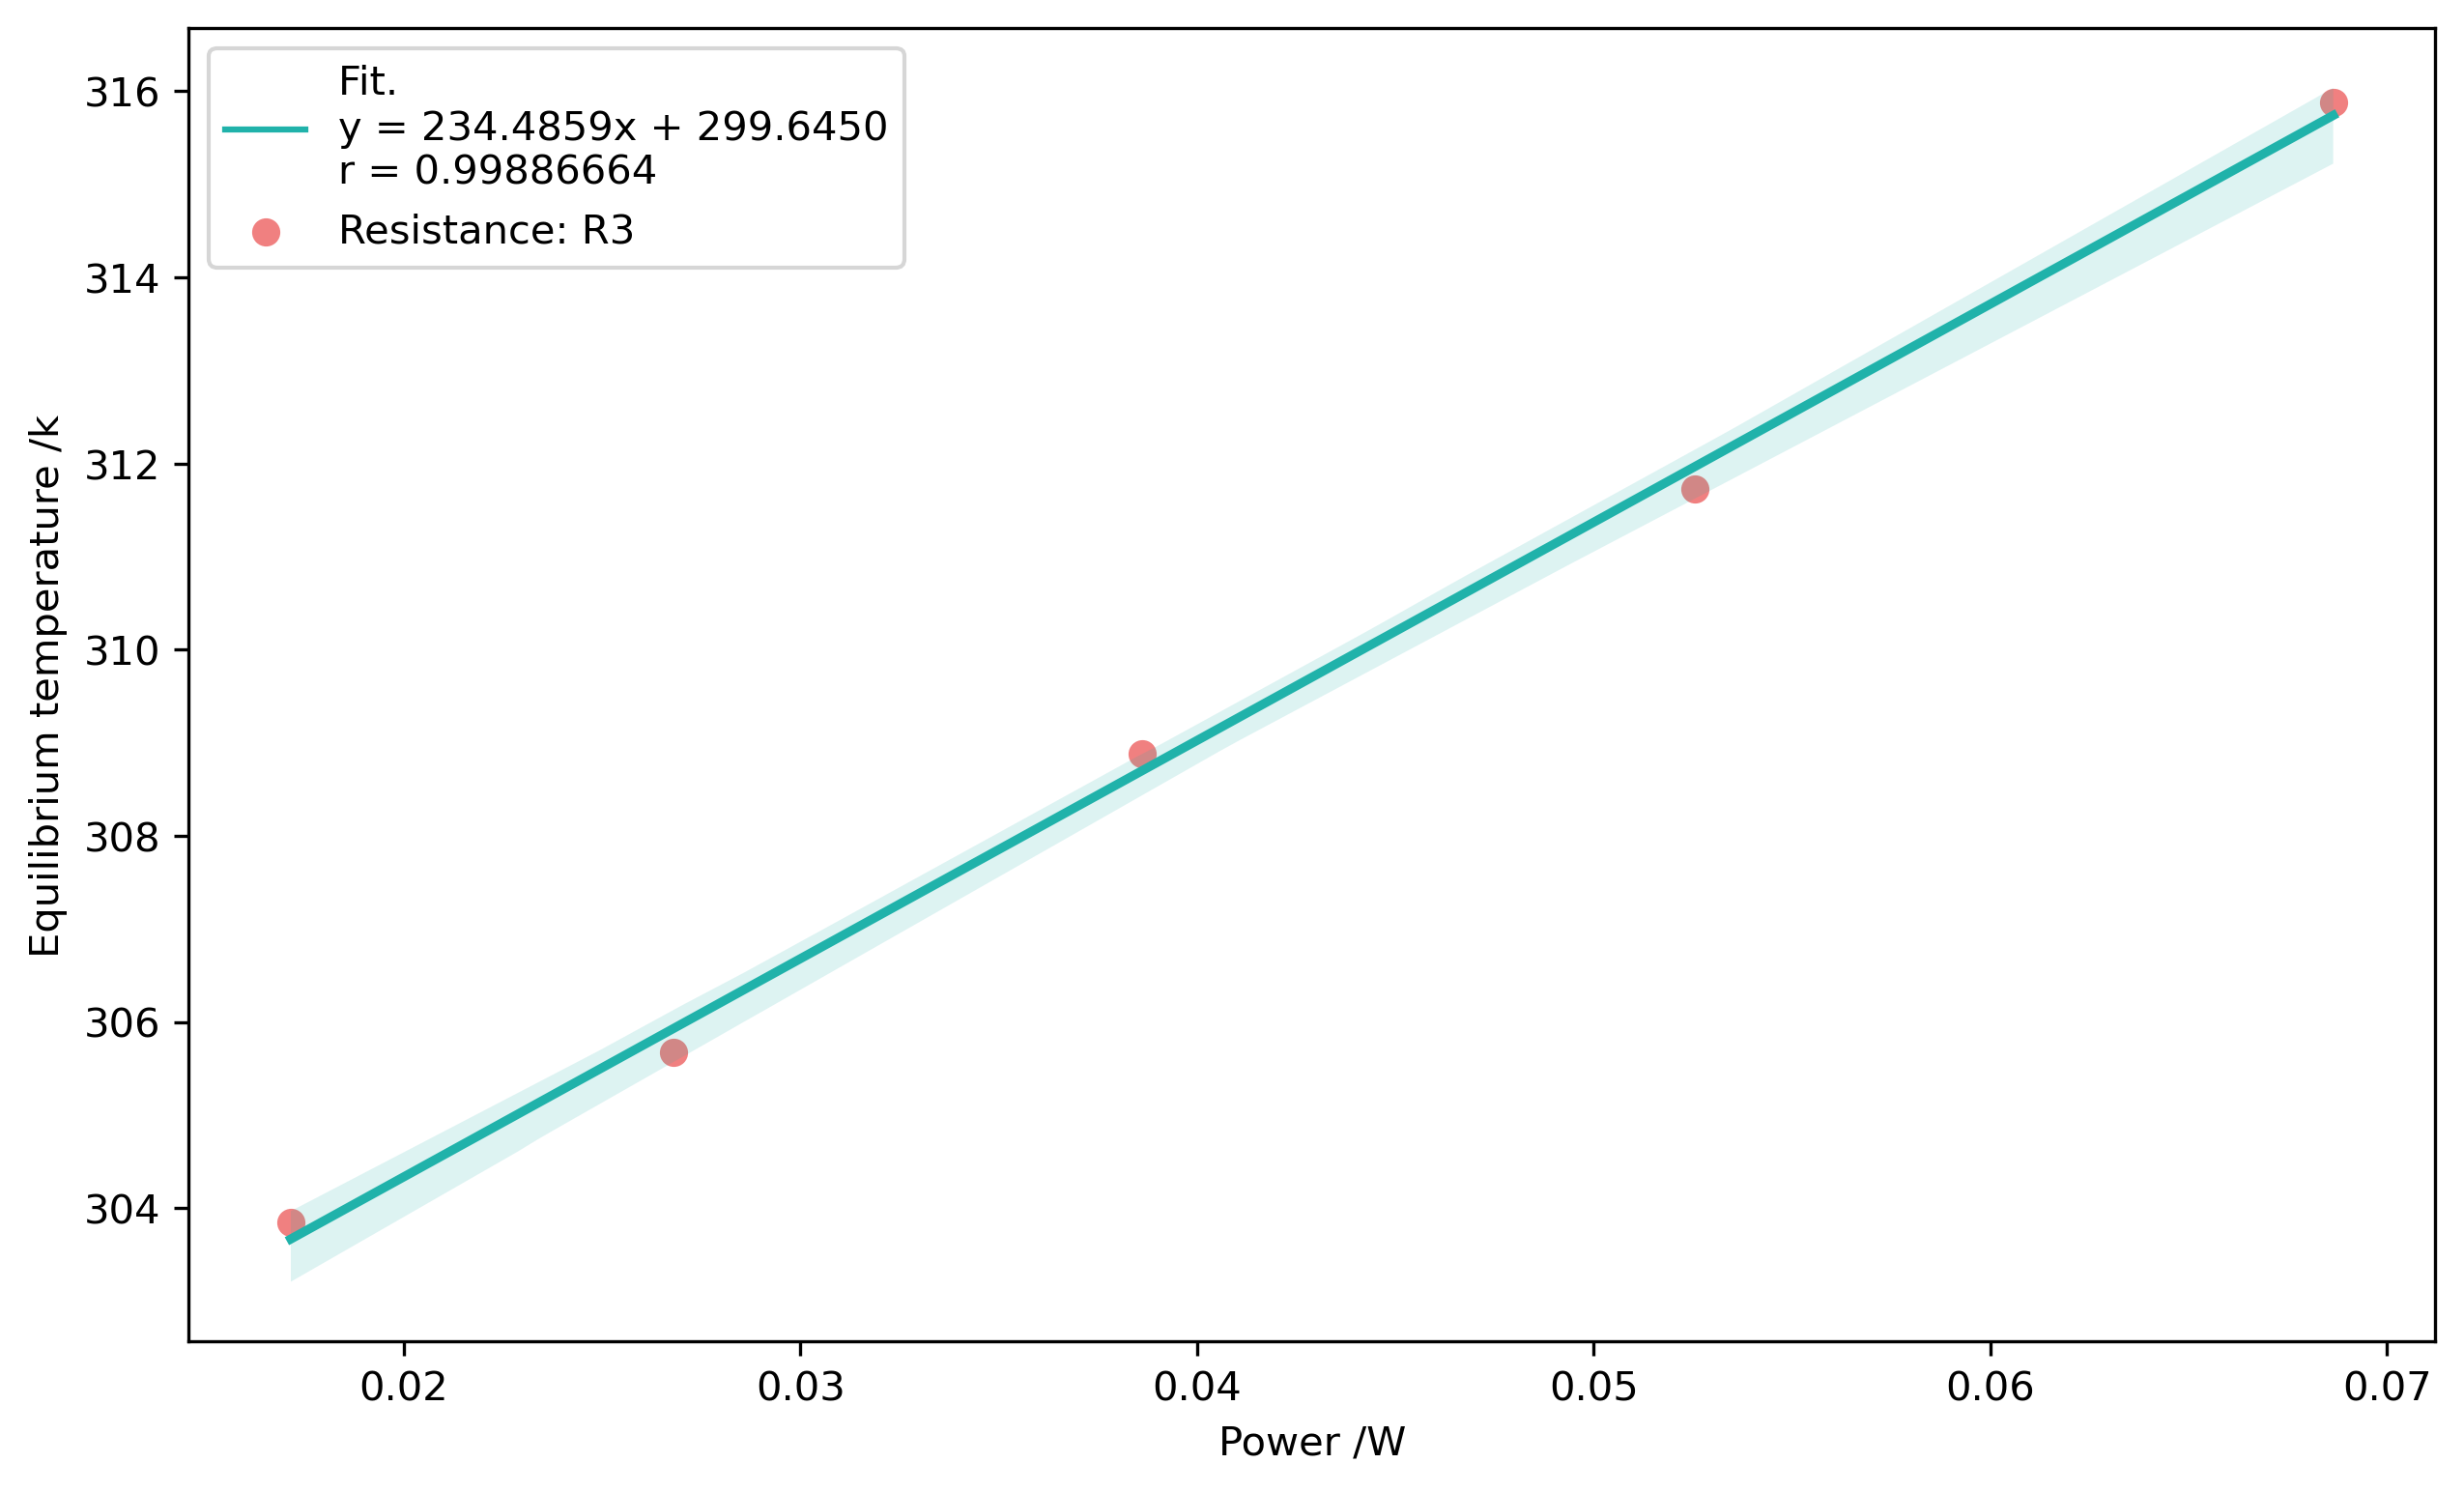
\includegraphics[width=0.3\textwidth]{attachments/fig.1.1.2.3.png}
		}
		\subfloat[$R_4 = 19.846 \Omega$]{\label{fig.1.1.2.4}
		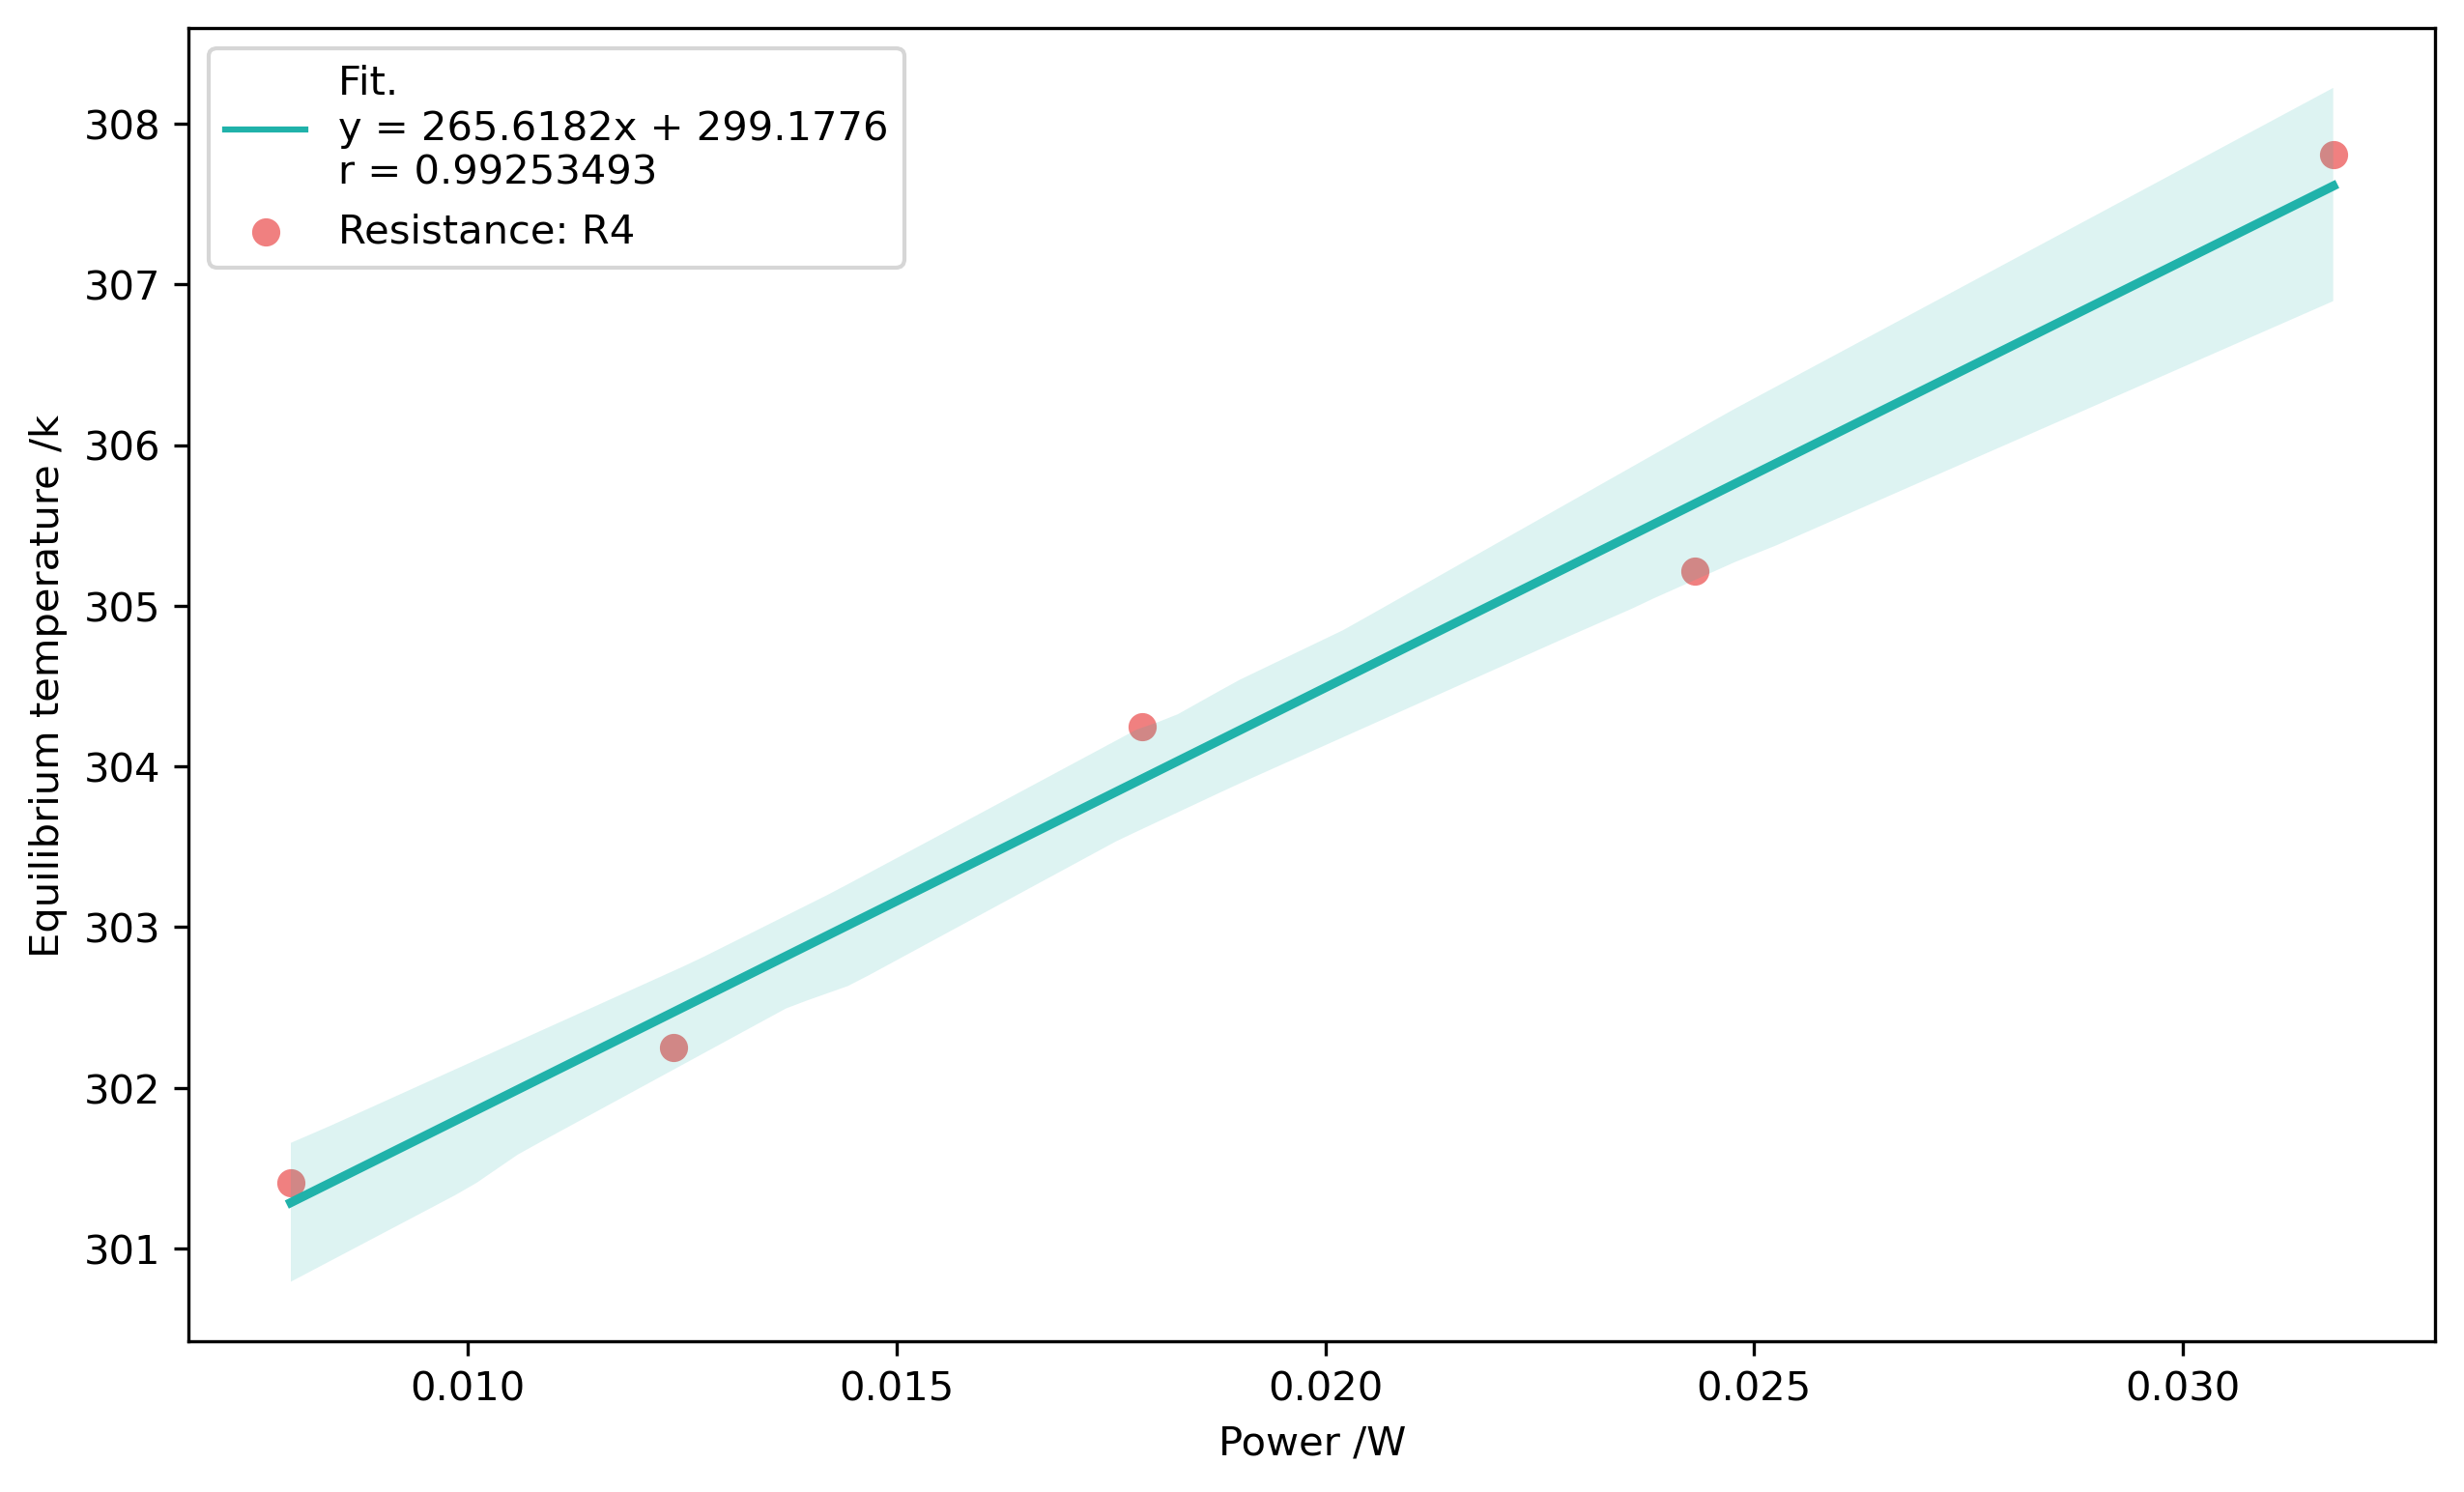
\includegraphics[width=0.3\textwidth]{attachments/fig.1.1.2.4.png}
		}
		\caption{\textbf{Correlation of equilibrium temperature and the heating power, real-world experiments}}
		\label{fig.1.1.2}
	\end{figure*}


	\paragraph{B1. Simulation: The ideal model}~
	\newline 
	\indent
	To begin with, we first built the ideal resistor thermal model (As illustrated in Fig. \ref{fig.illus-1.1}) and run the simulation on COMSOL platform.
	The geometric model of the ideal resistor thermal model is shown in Fig. \ref{fig.1.2.0}. 
	The top and bottom surfaces of the resistor were set as adiabatic, and the side faces were able to exchange heat with surroundings following the Newton's cooling law. 
	With different currents provided, the heating curves were obtained(Fig. \ref{fig.1.2.1}),
	and the correlation of the equilibrium temperatures of each resistor and the heating powers were shown in Fig. \ref{fig.1.2.2}.

	Results show that the equilibrium temperature was directly proportional to the resist value, which is consistent with the real-world experiment.

	\begin{figure*}[htbp]
		\centering
		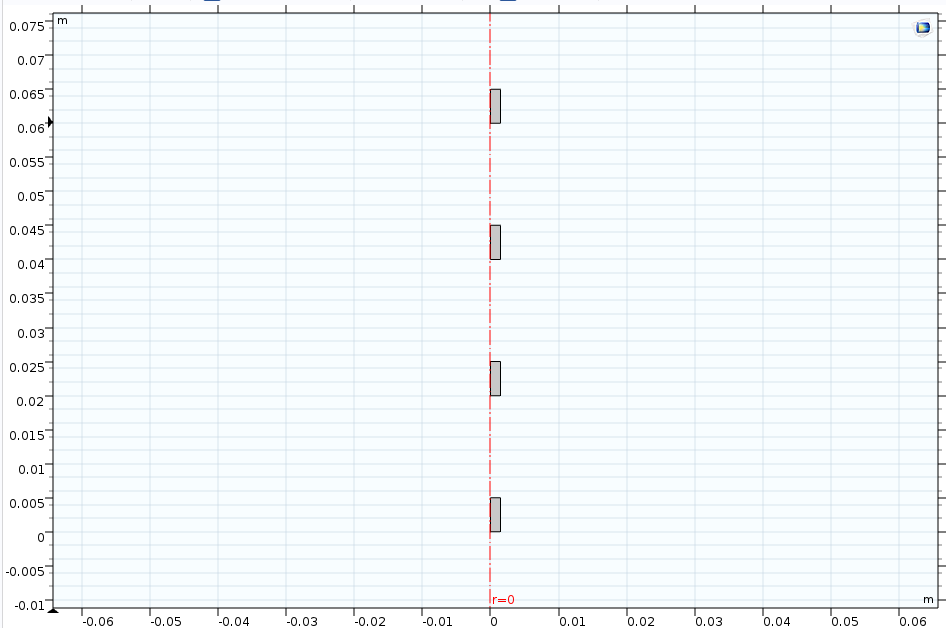
\includegraphics[width=0.3\textwidth]{attachments/fig.1.2.0.png}
		\caption{\textbf{The geometric model of the ideal resistor model}}
		\label{fig.1.2.0}
	\end{figure*}
	
	\begin{figure*}[htbp]
		\centering
		\subfloat[$I=0.020A$]{\label{fig.1.2.1.1}
		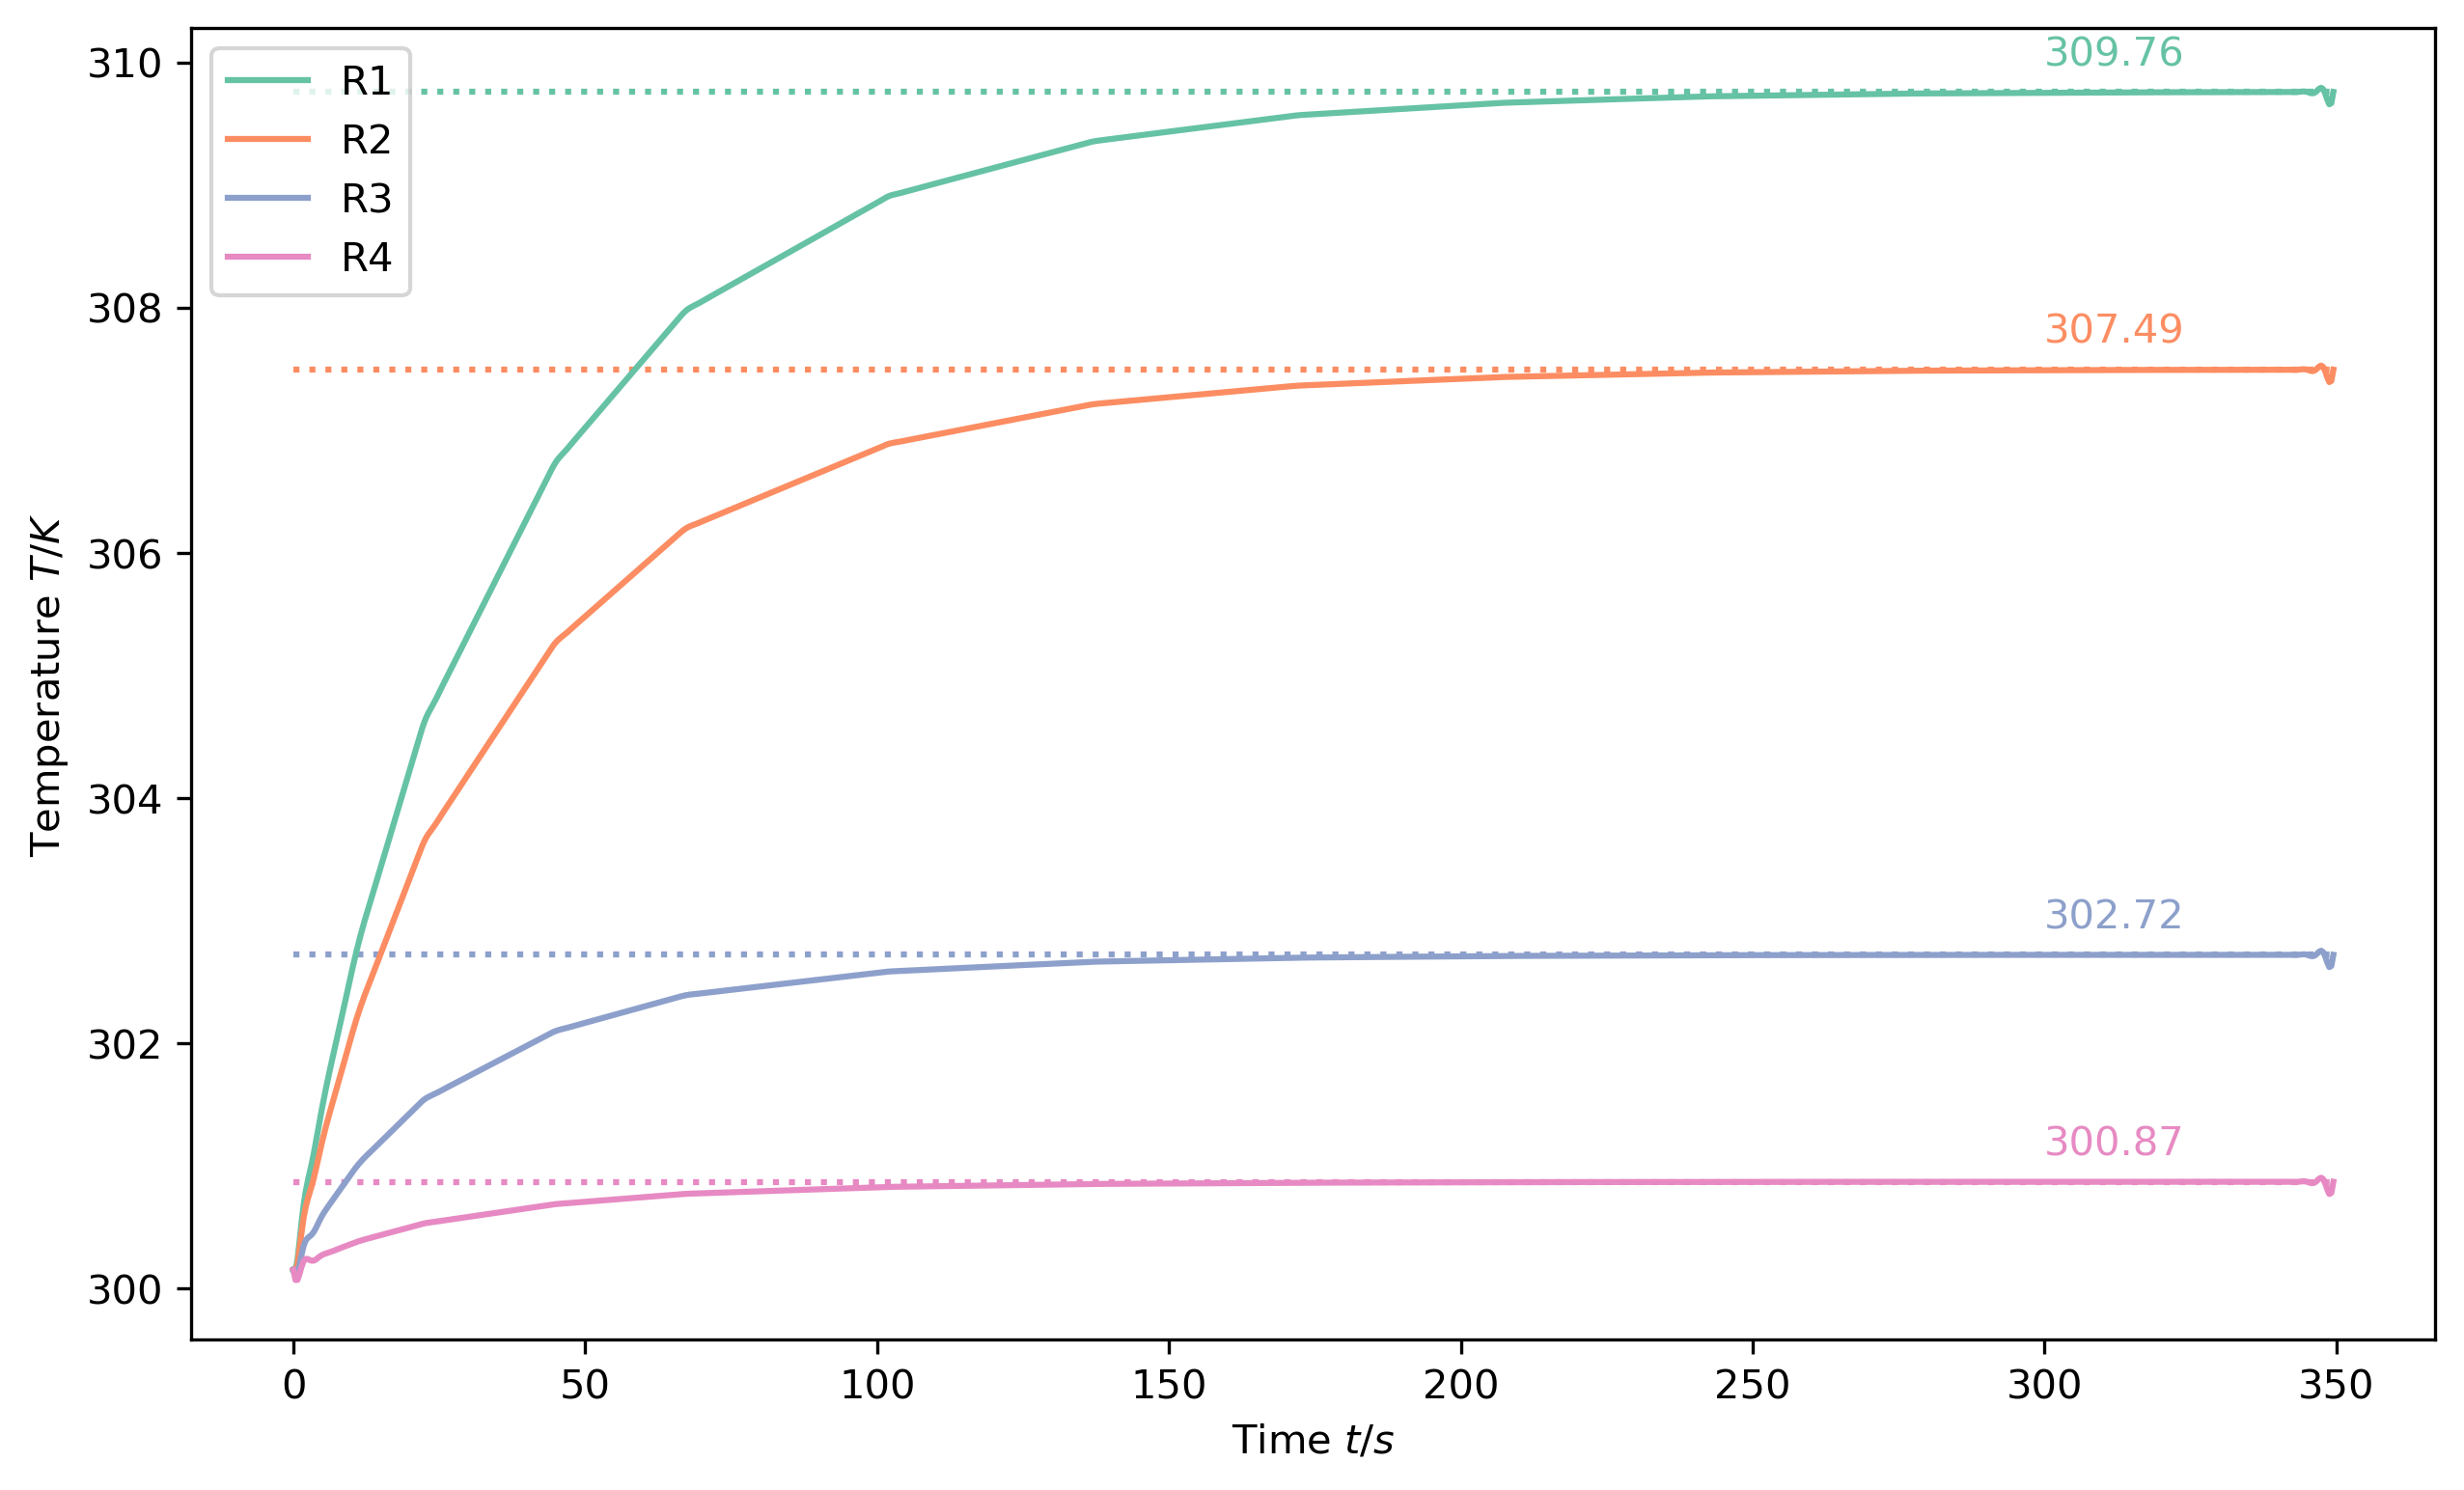
\includegraphics[width=0.3\textwidth]{attachments/fig.1.2.1.1.png}
		}		
		\subfloat[$I=0.025A$]{\label{fig.1.2.1.2}
		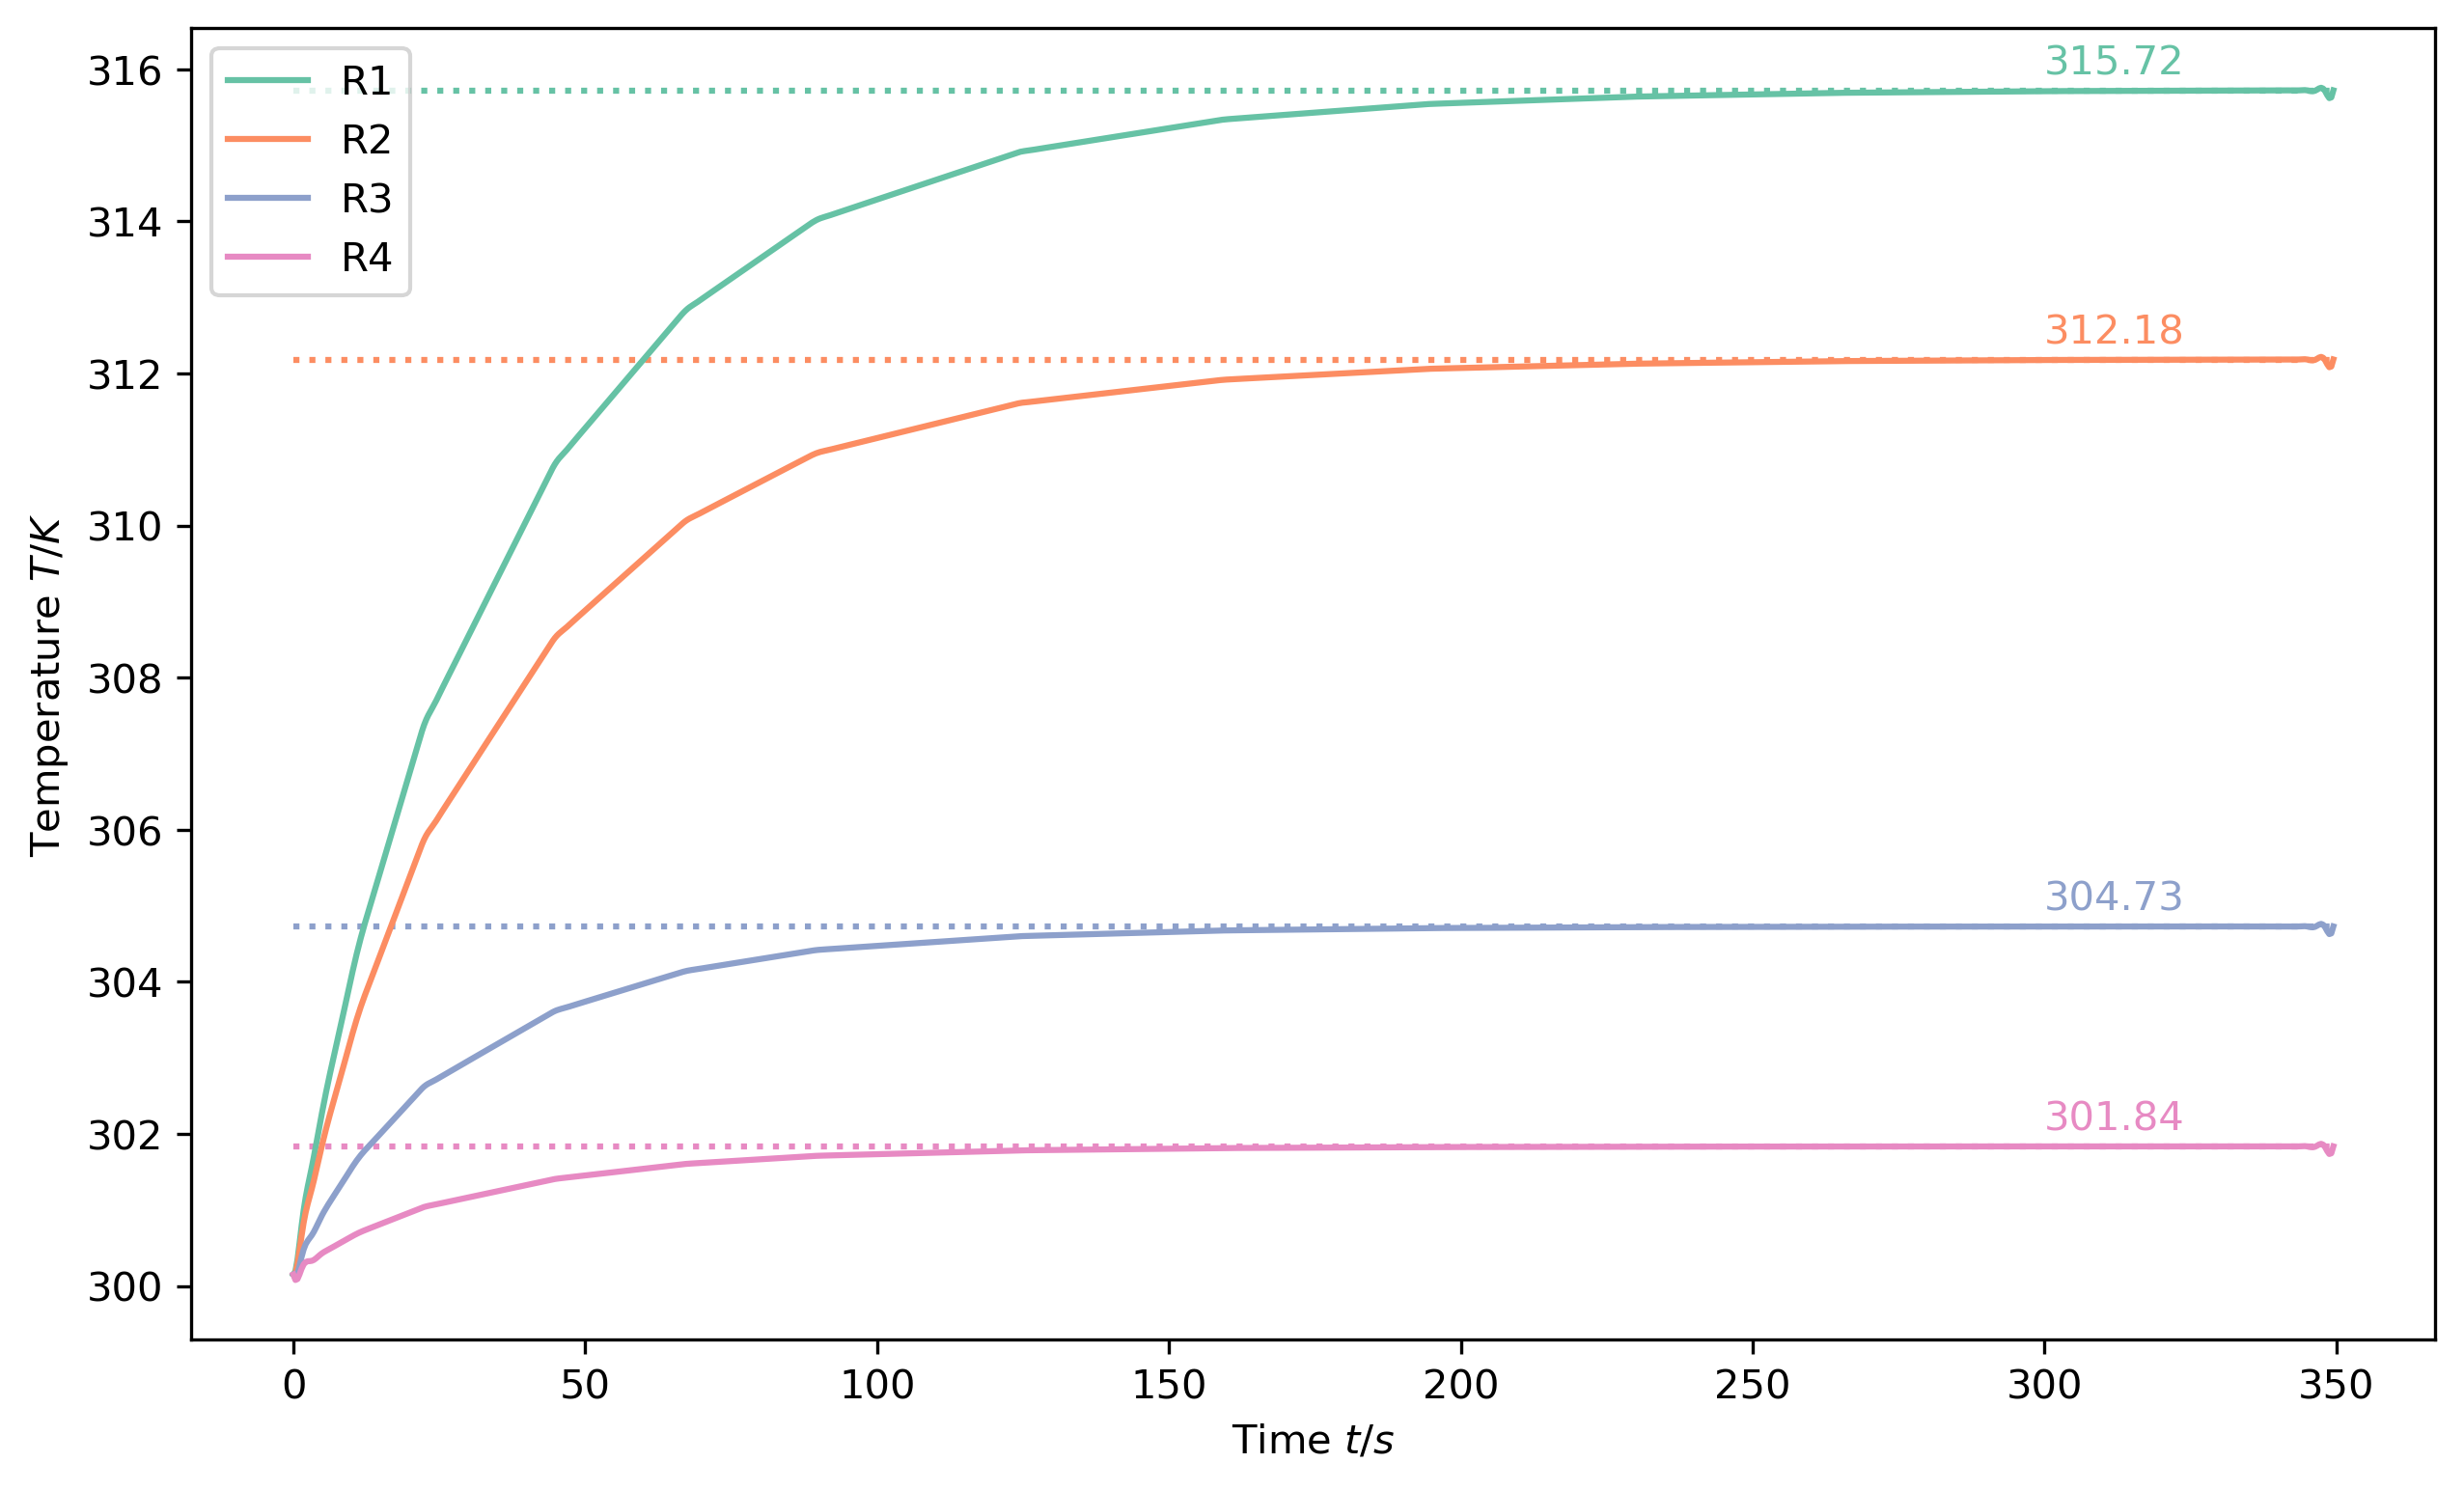
\includegraphics[width=0.3\textwidth]{attachments/fig.1.2.1.2.png}
		}

		\subfloat[$I=0.030A$]{\label{fig.1.2.1.3}
		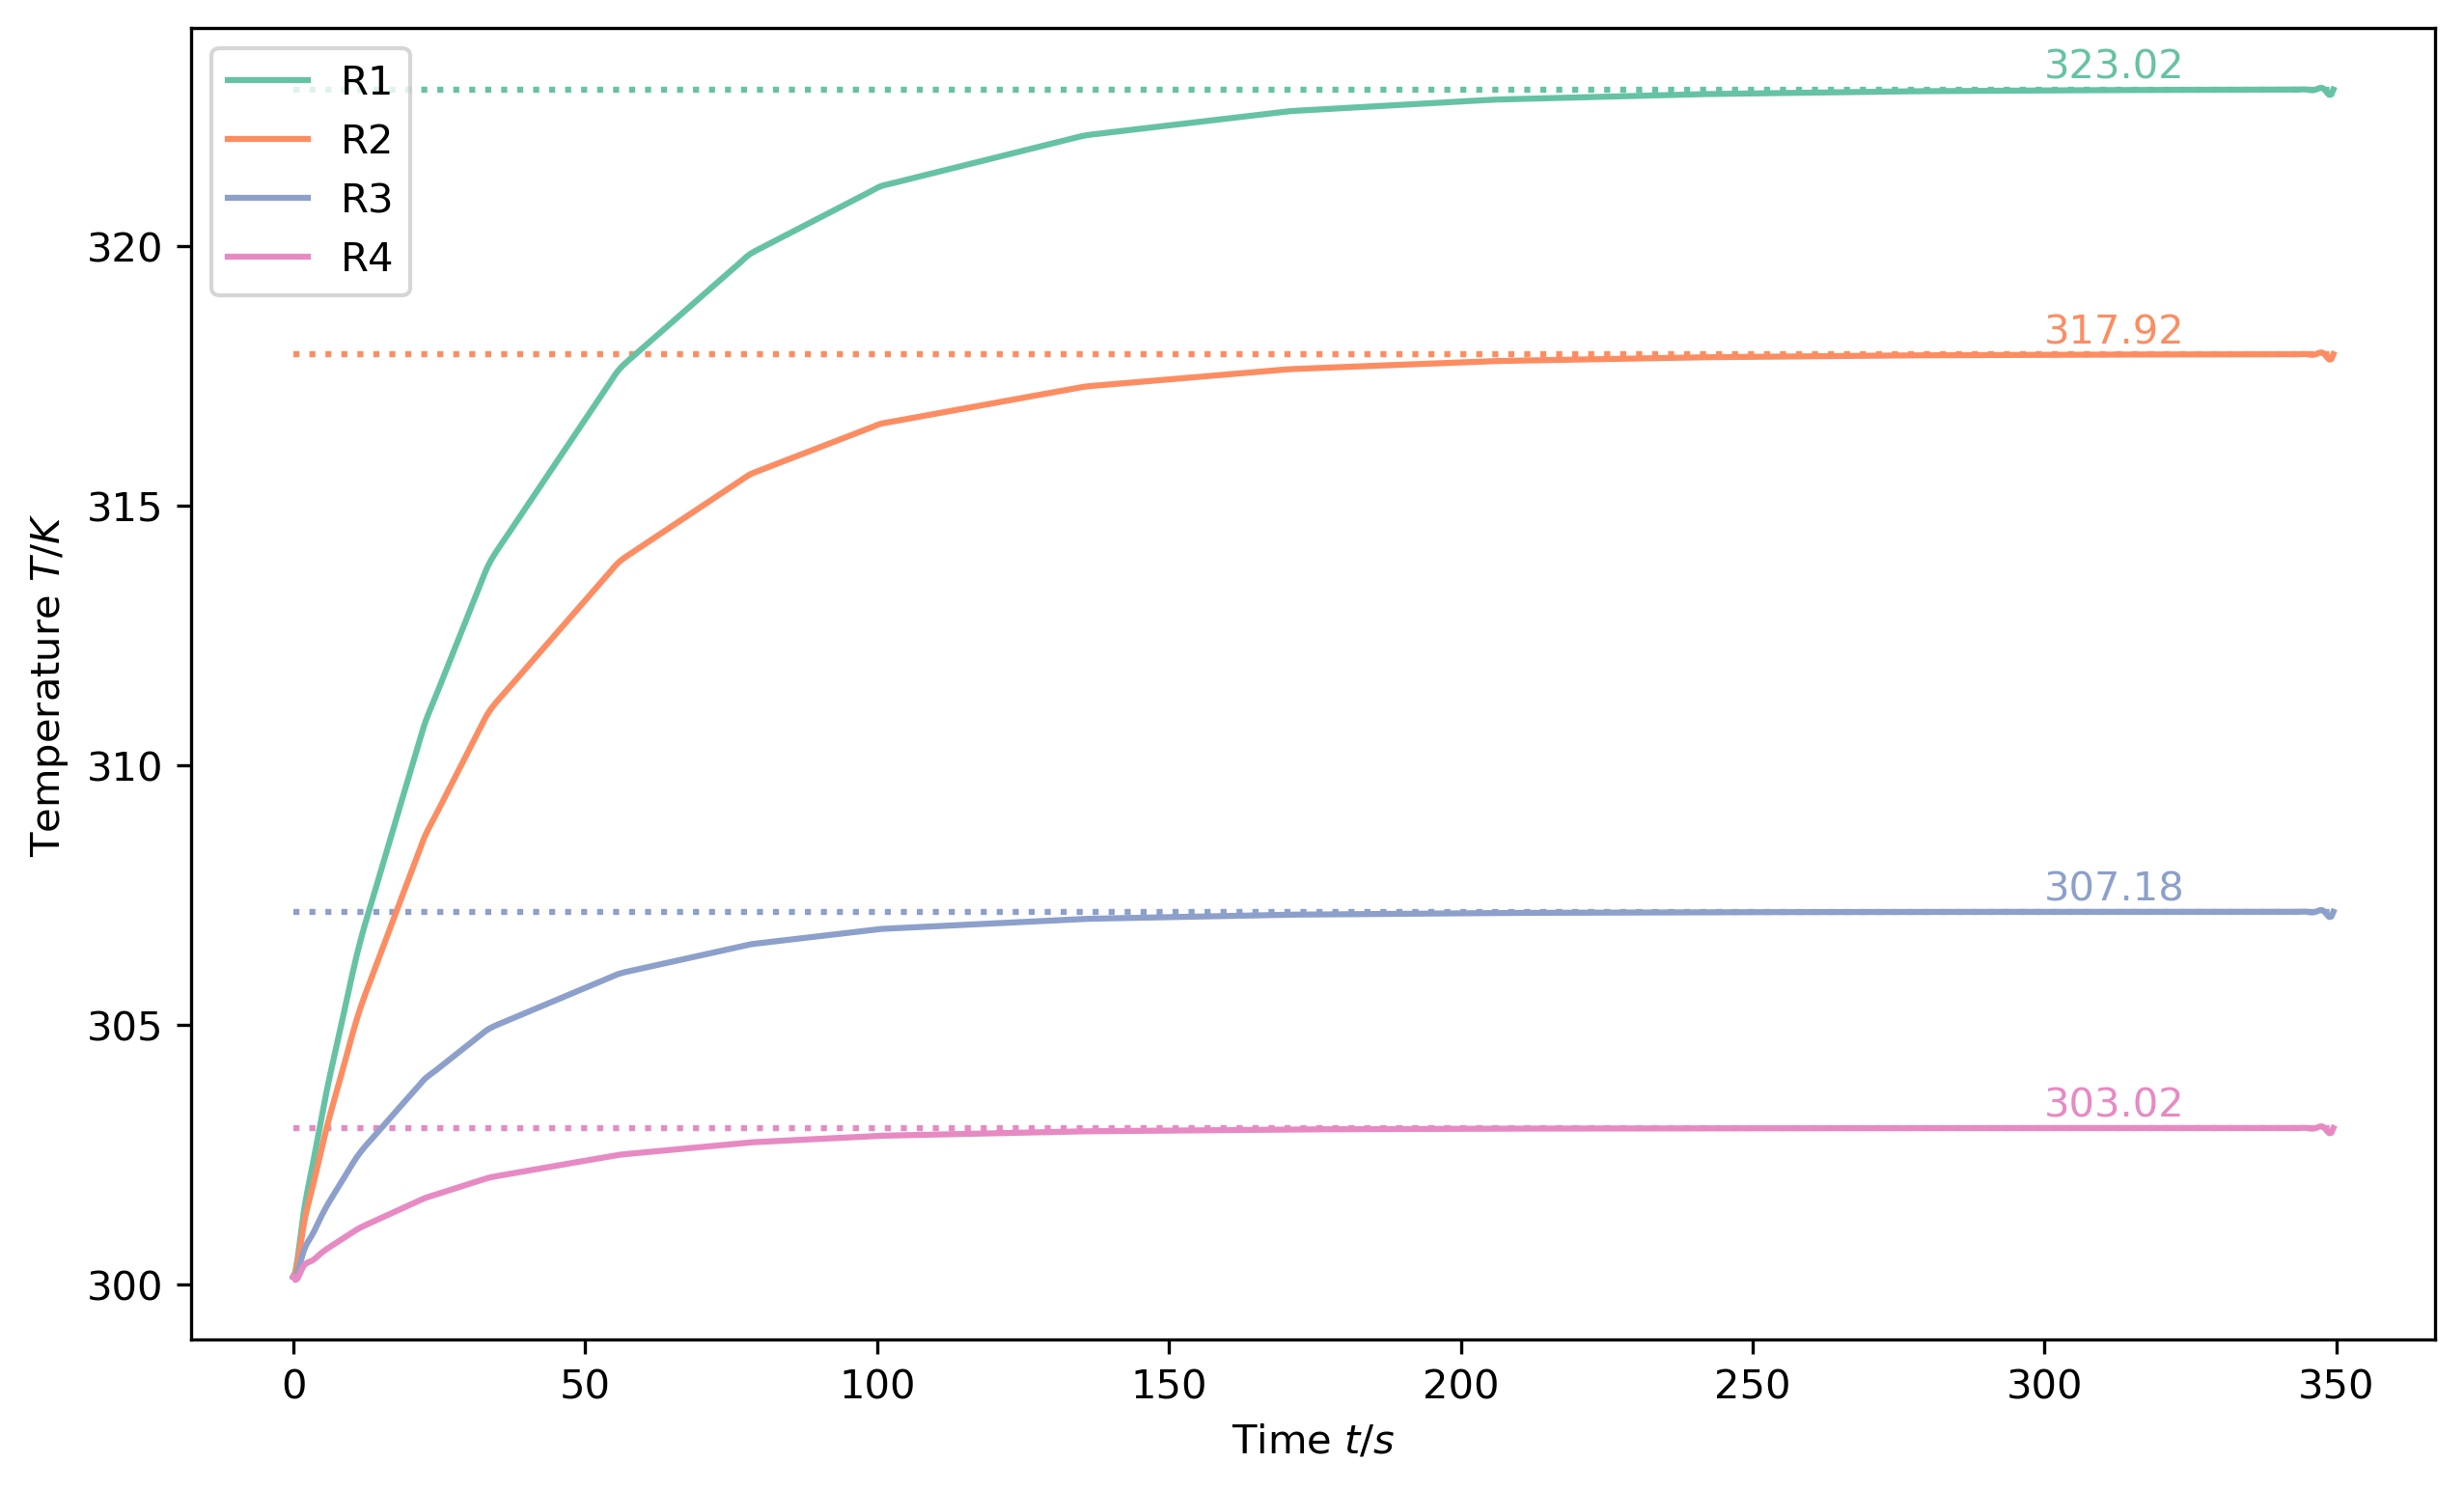
\includegraphics[width=0.3\textwidth]{attachments/fig.1.2.1.3.png}
		}
		\subfloat[$I=0.035A$]{\label{fig.1.2.1.4}
		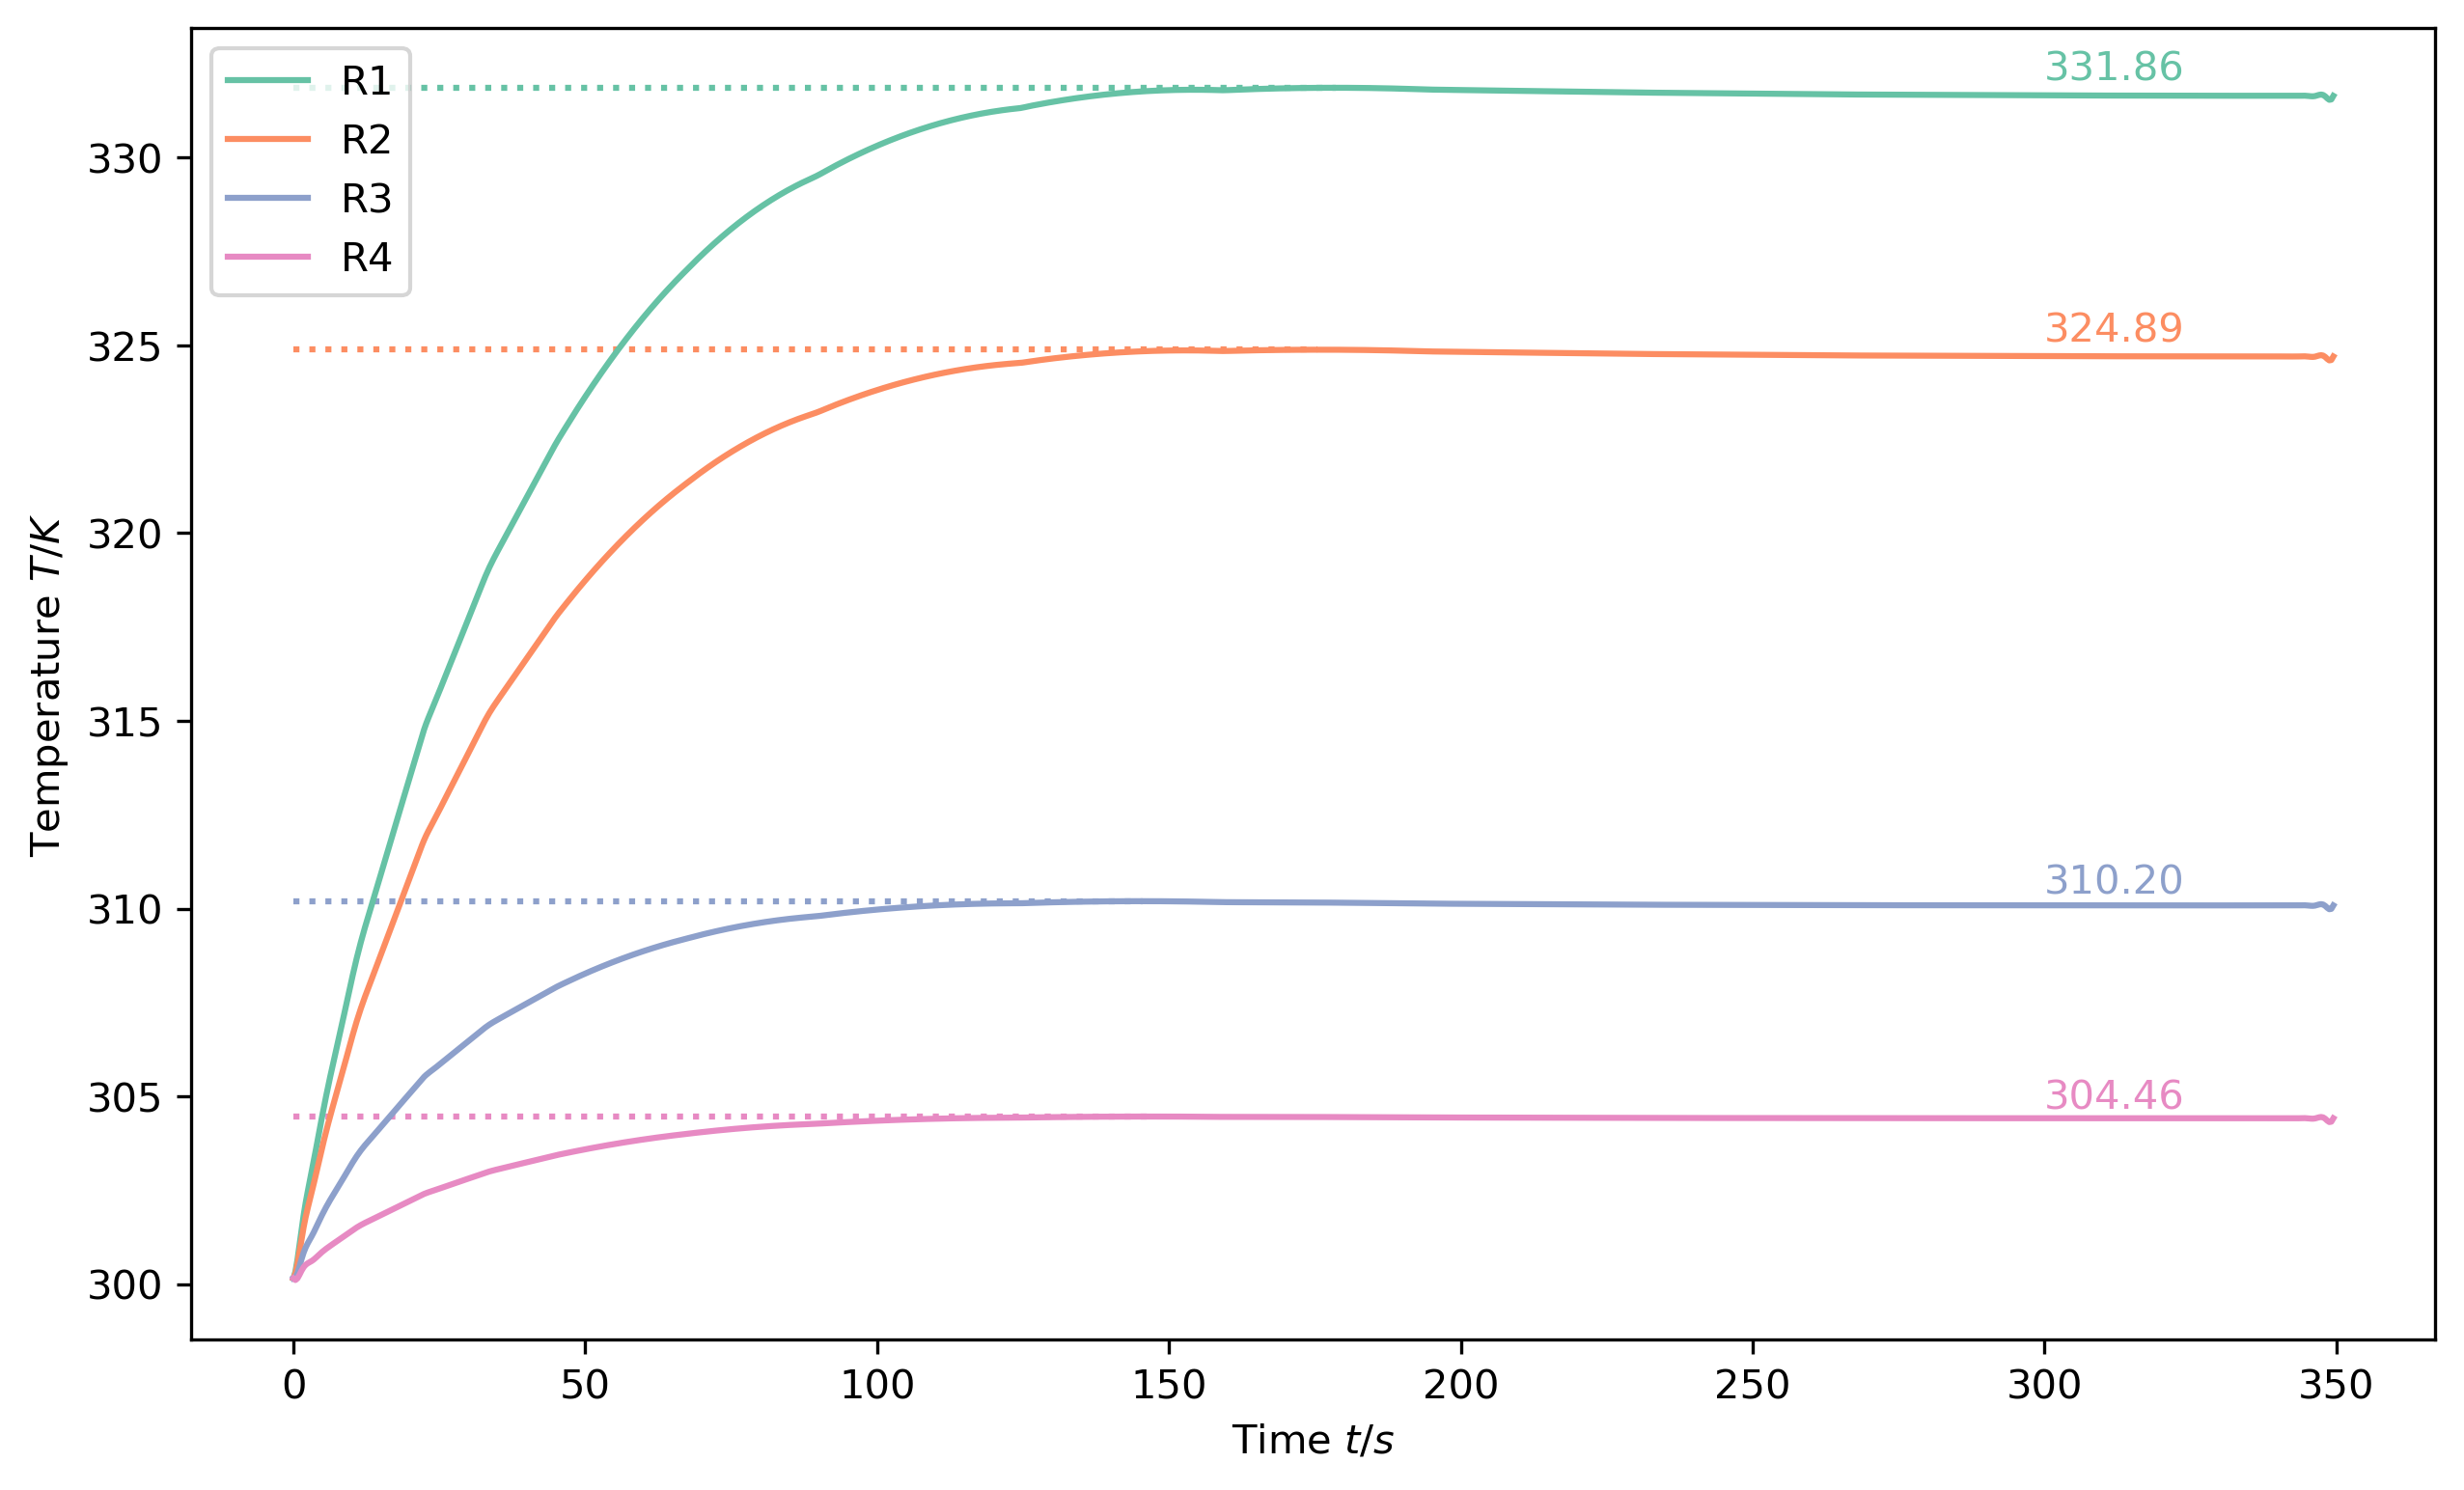
\includegraphics[width=0.3\textwidth]{attachments/fig.1.2.1.4.png}
		}
		\subfloat[$I=0.040A$]{\label{fig.1.2.1.5}
		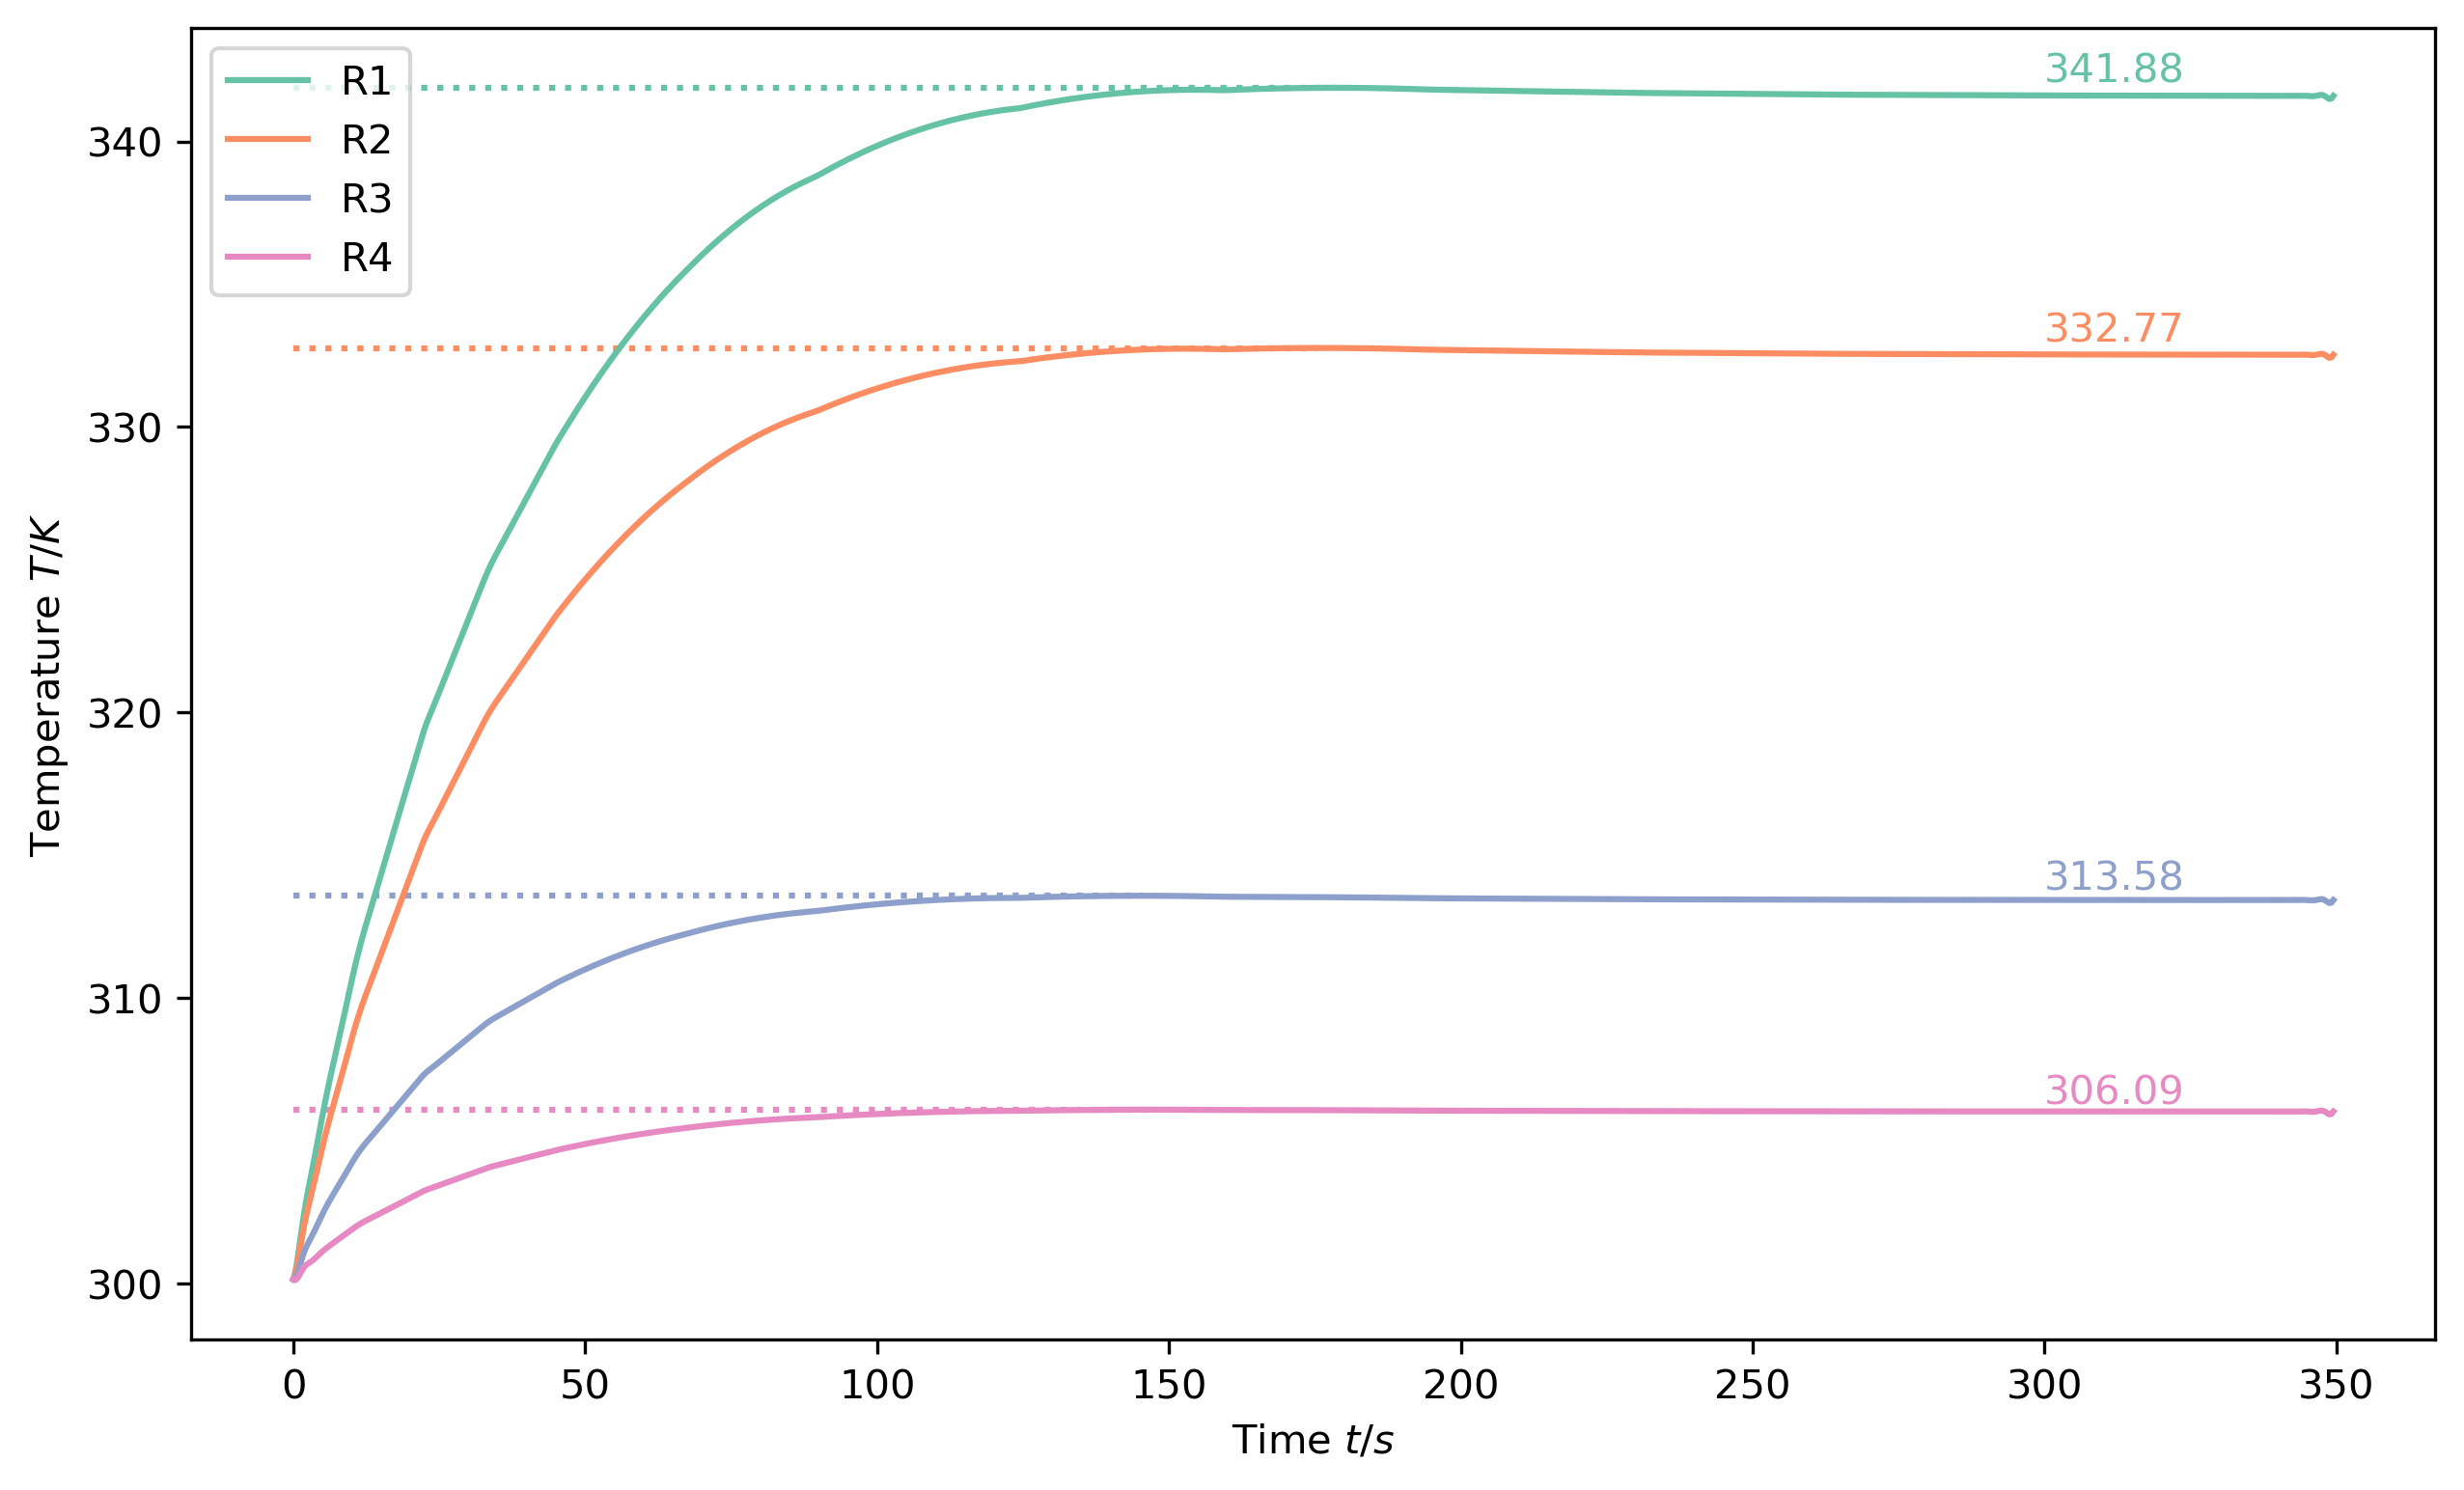
\includegraphics[width=0.3\textwidth]{attachments/fig.1.2.1.5.png}
		}
		\caption{\textbf{Heating curves of the series resistors under different currents, simulation experiments of the ideal model}}
		\label{fig.1.2.1}
	\end{figure*}

	\begin{figure*}[htbp]
		\centering
		\subfloat[$R_1 = 100.00 \Omega$]{\label{fig.1.2.2.1}
		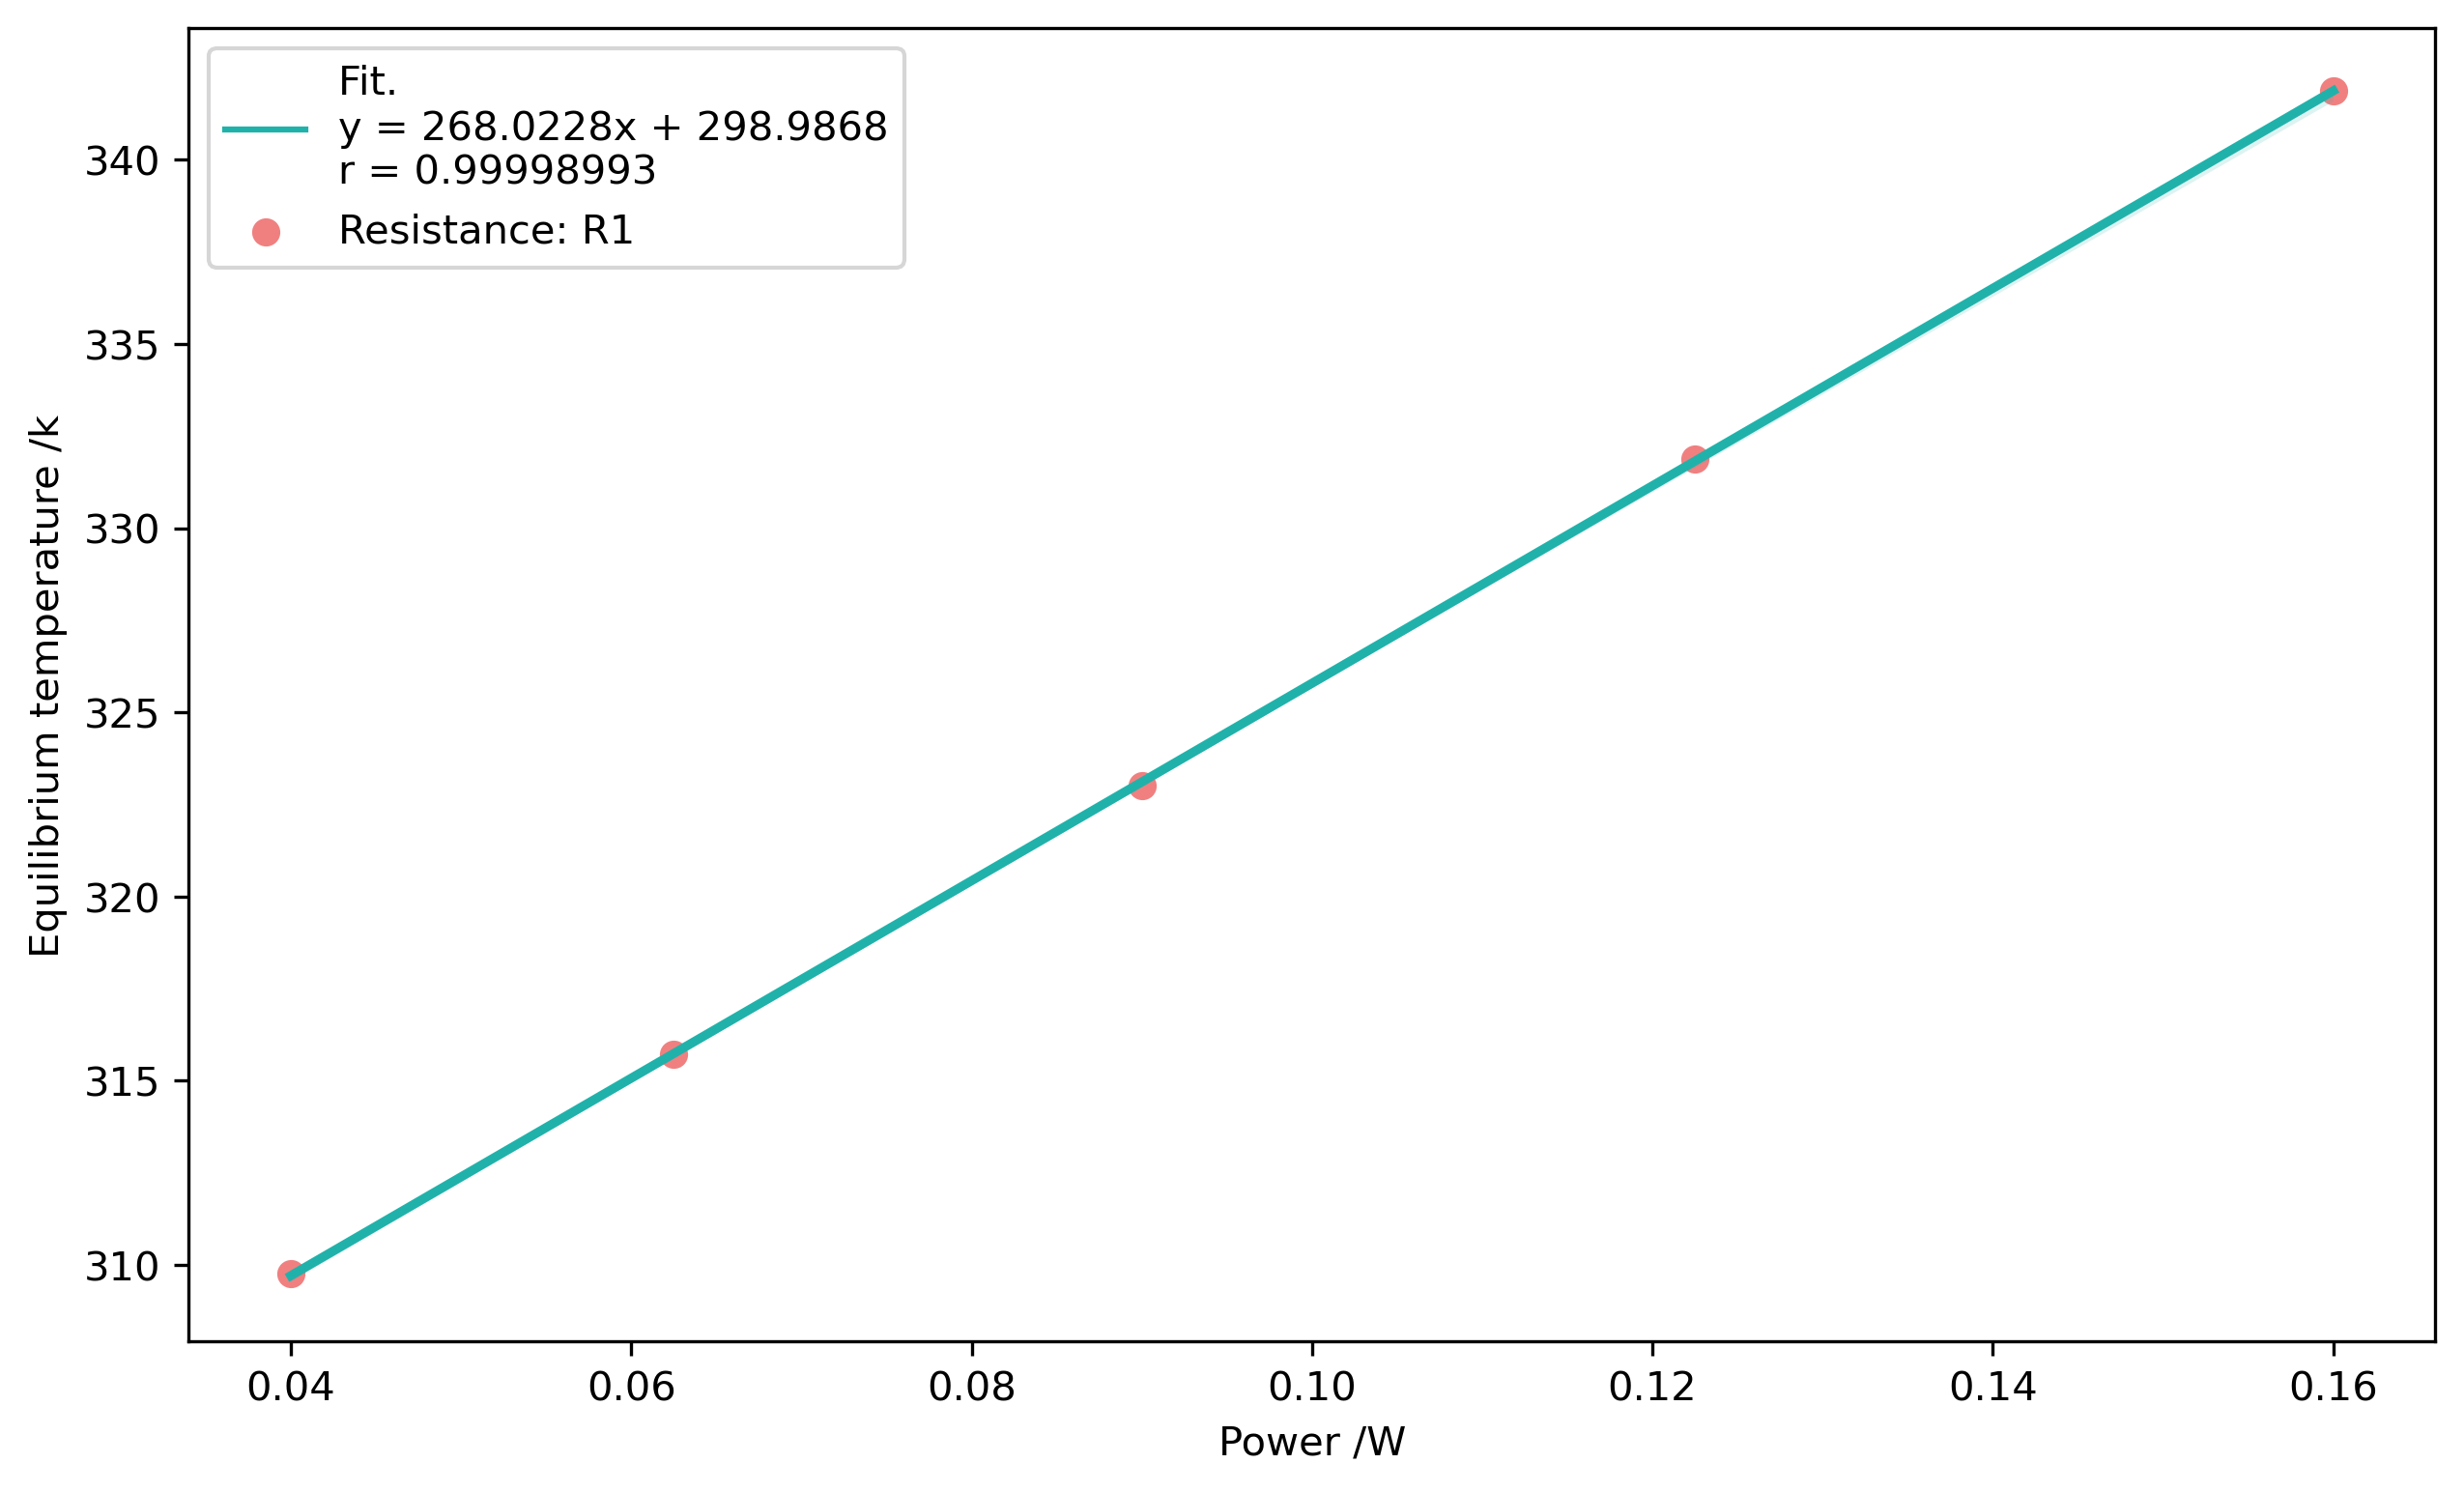
\includegraphics[width=0.3\textwidth]{attachments/fig.1.2.2.1.png}
		}		
		\subfloat[$R_2 = 81.588 \Omega$]{\label{fig.1.2.2.2}
		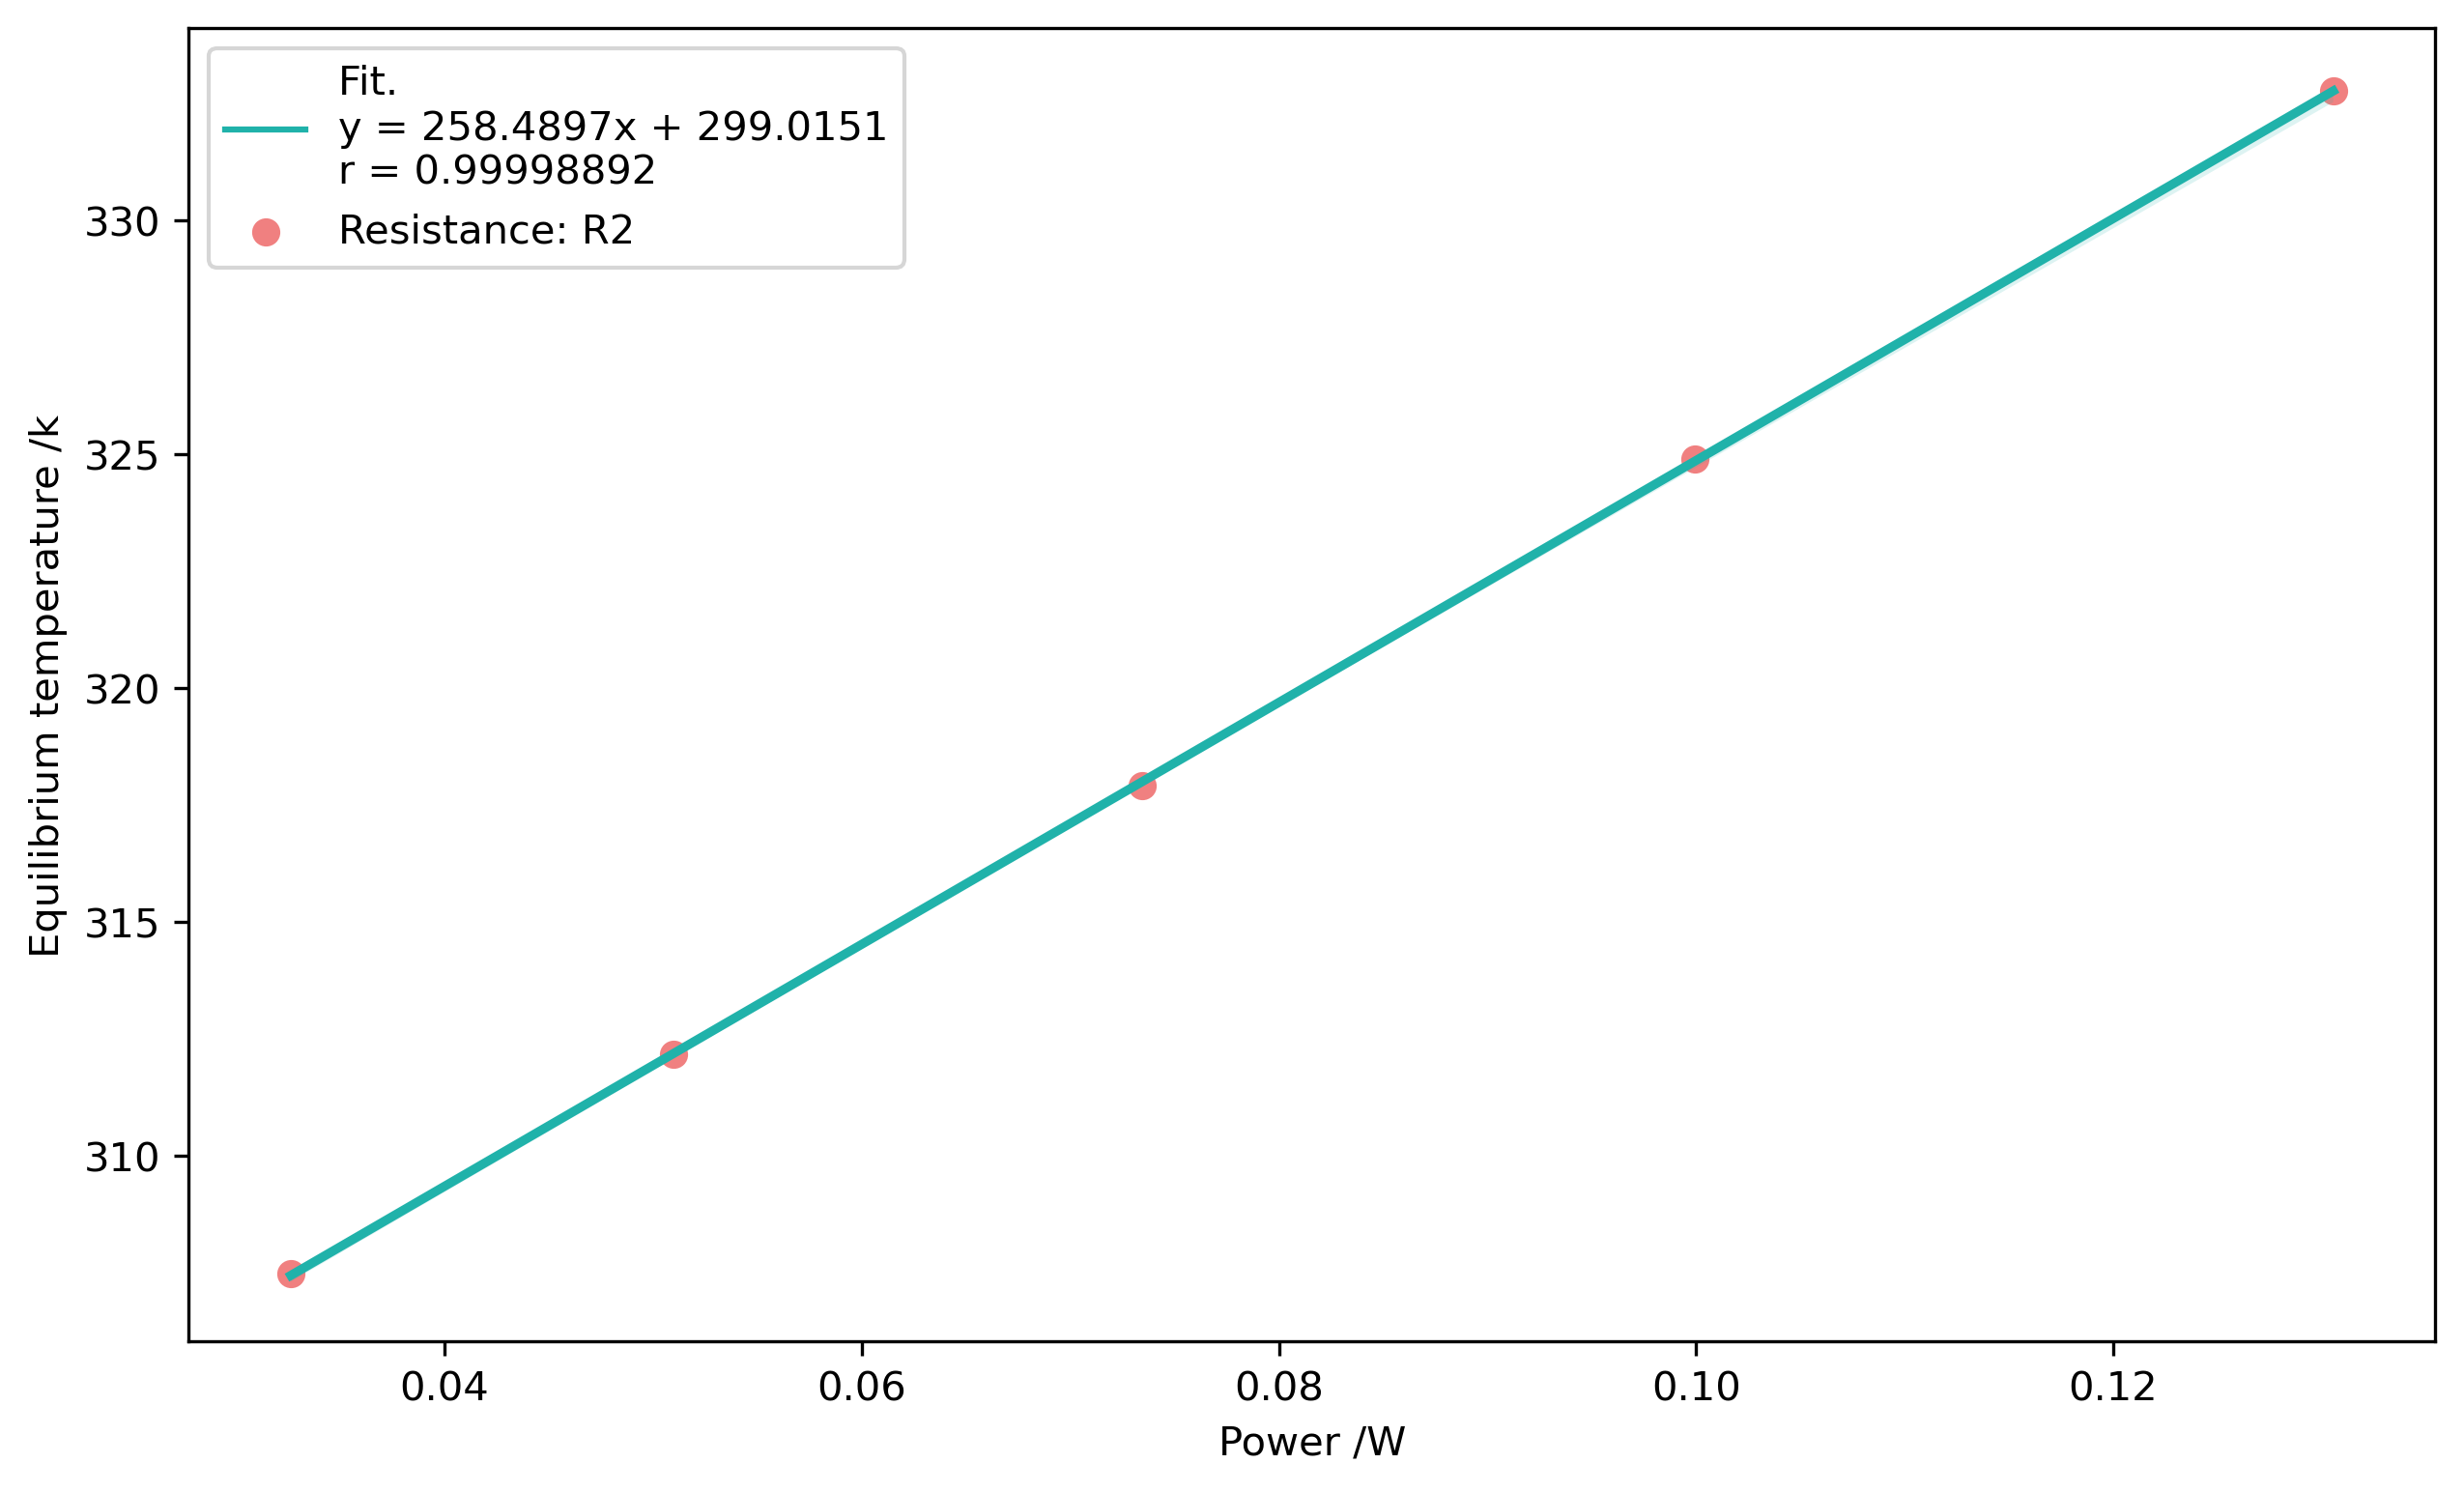
\includegraphics[width=0.3\textwidth]{attachments/fig.1.2.2.2.png}
		}

		\subfloat[$R_3 = 42.902 \Omega$]{\label{fig.1.2.2.3}
		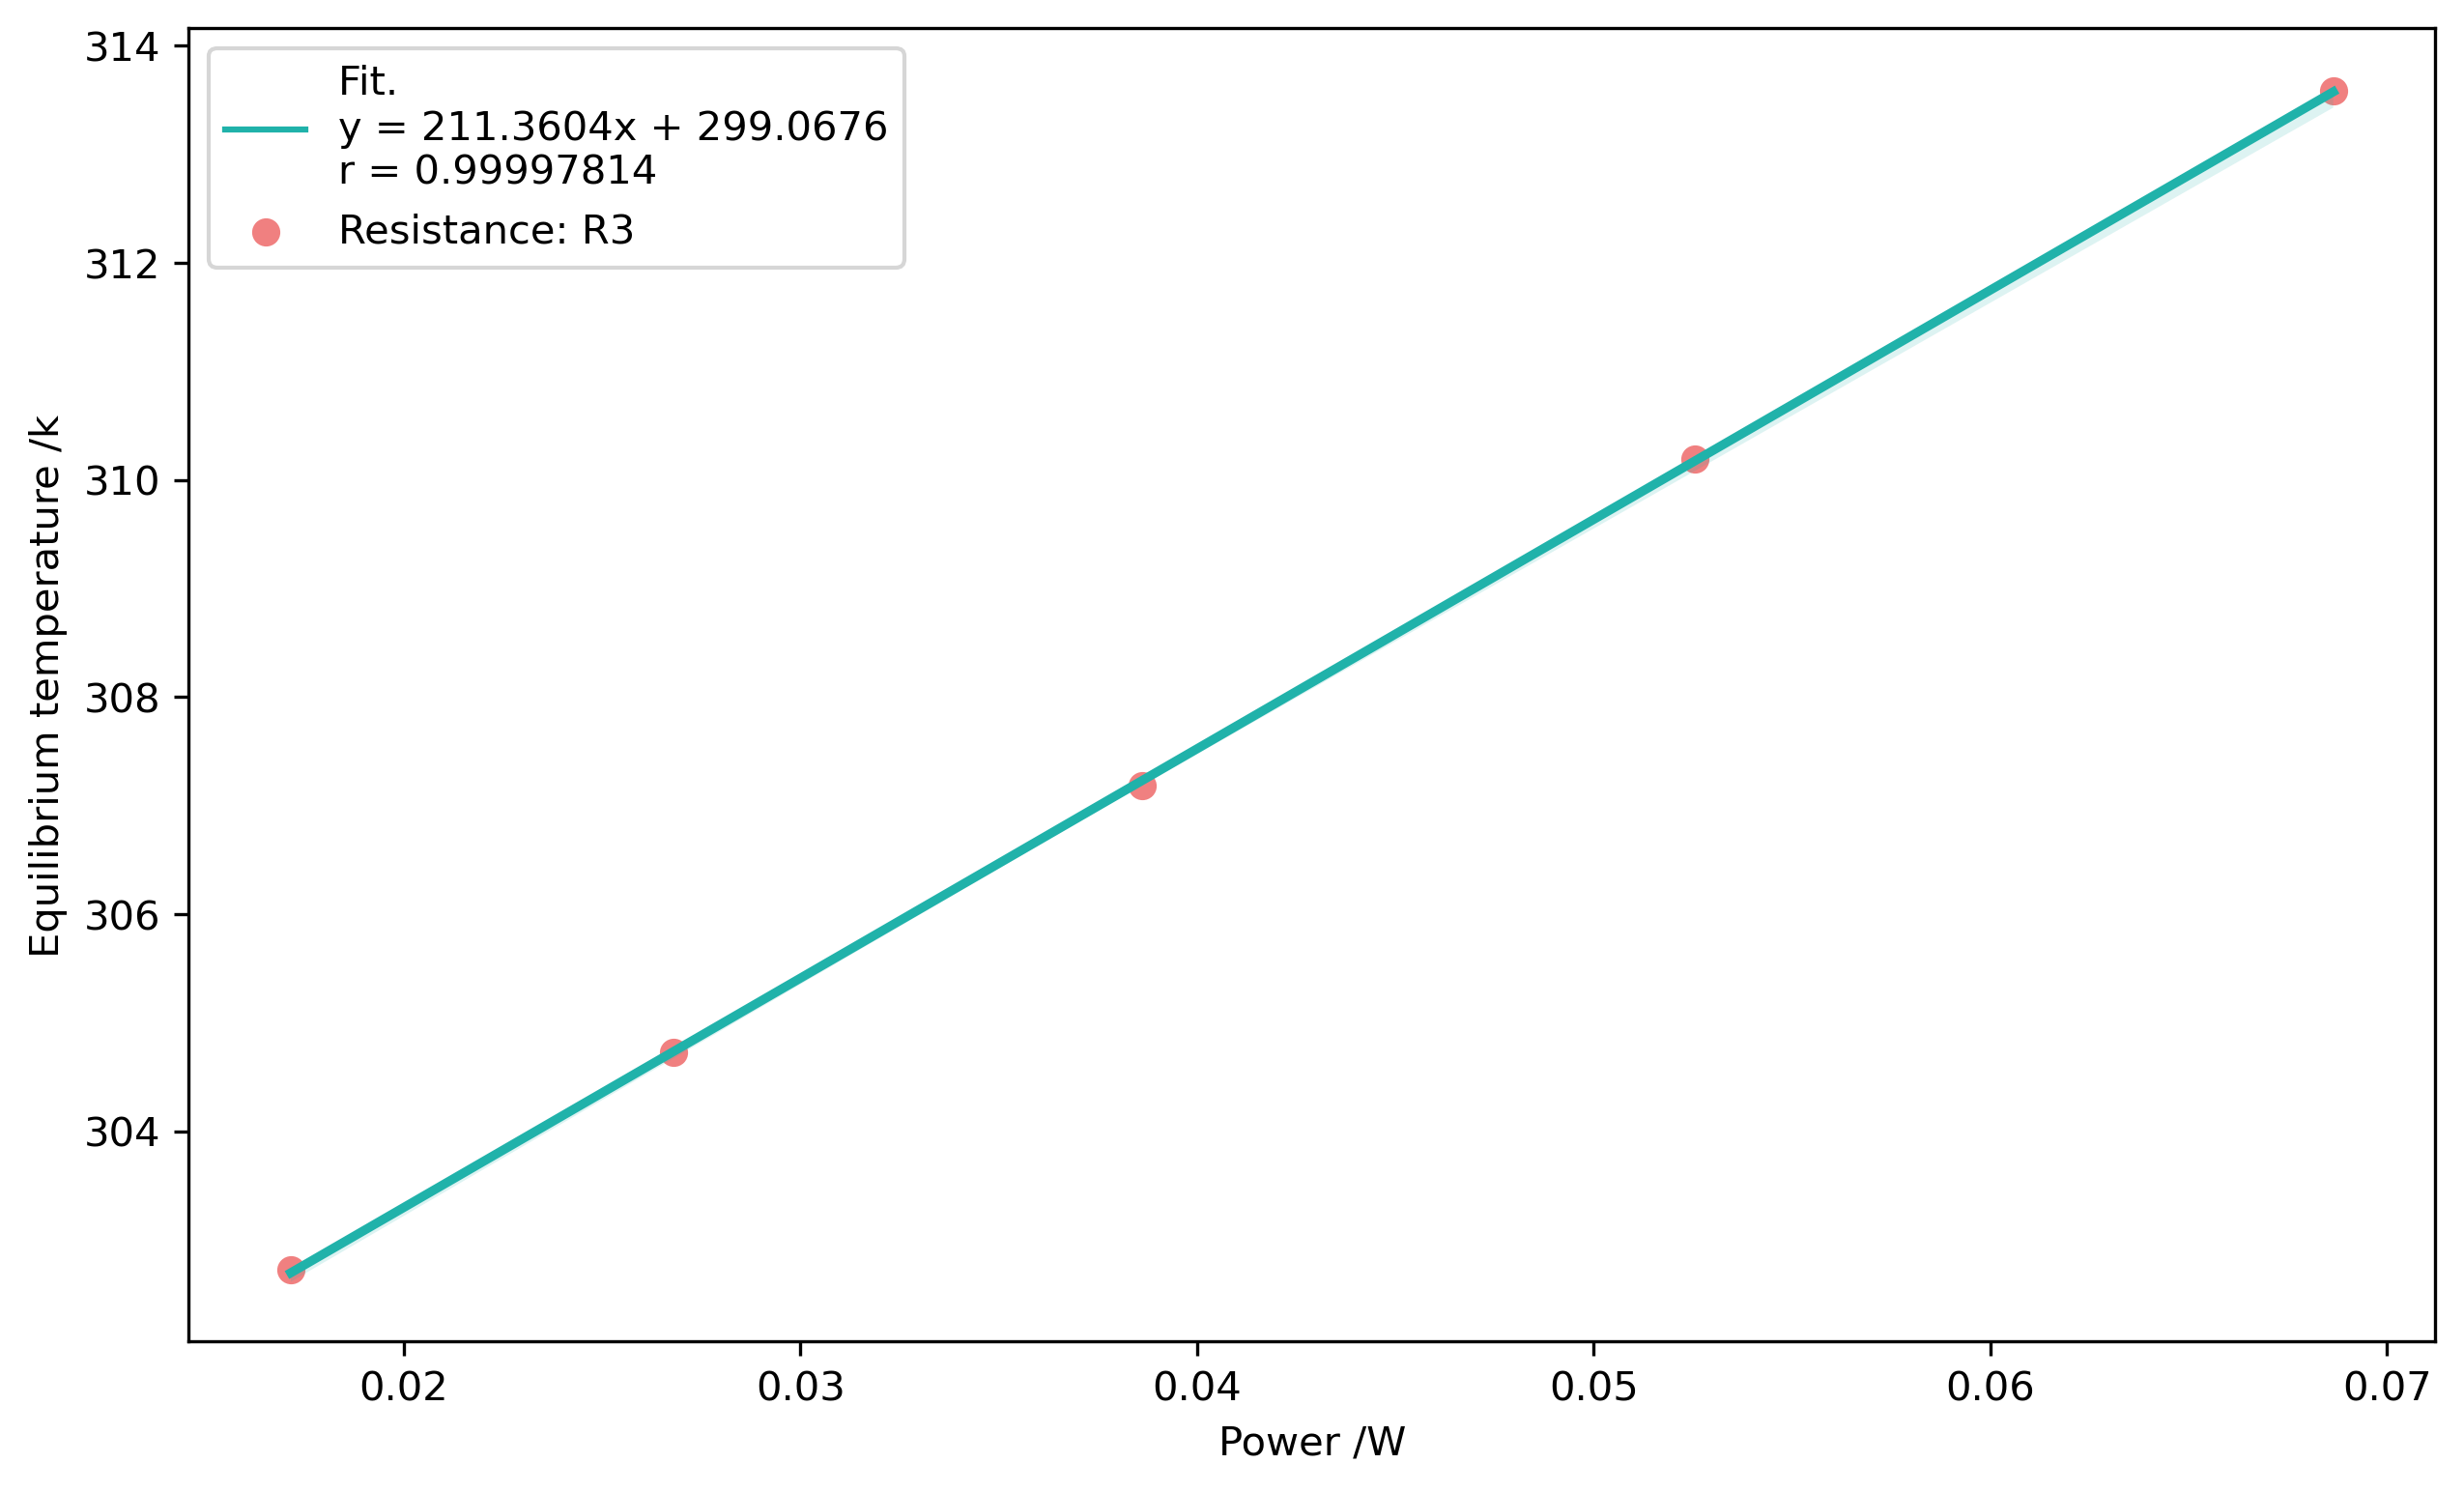
\includegraphics[width=0.3\textwidth]{attachments/fig.1.2.2.3.png}
		}
		\subfloat[$R_4 = 19.846 \Omega$]{\label{fig.1.2.2.4}
		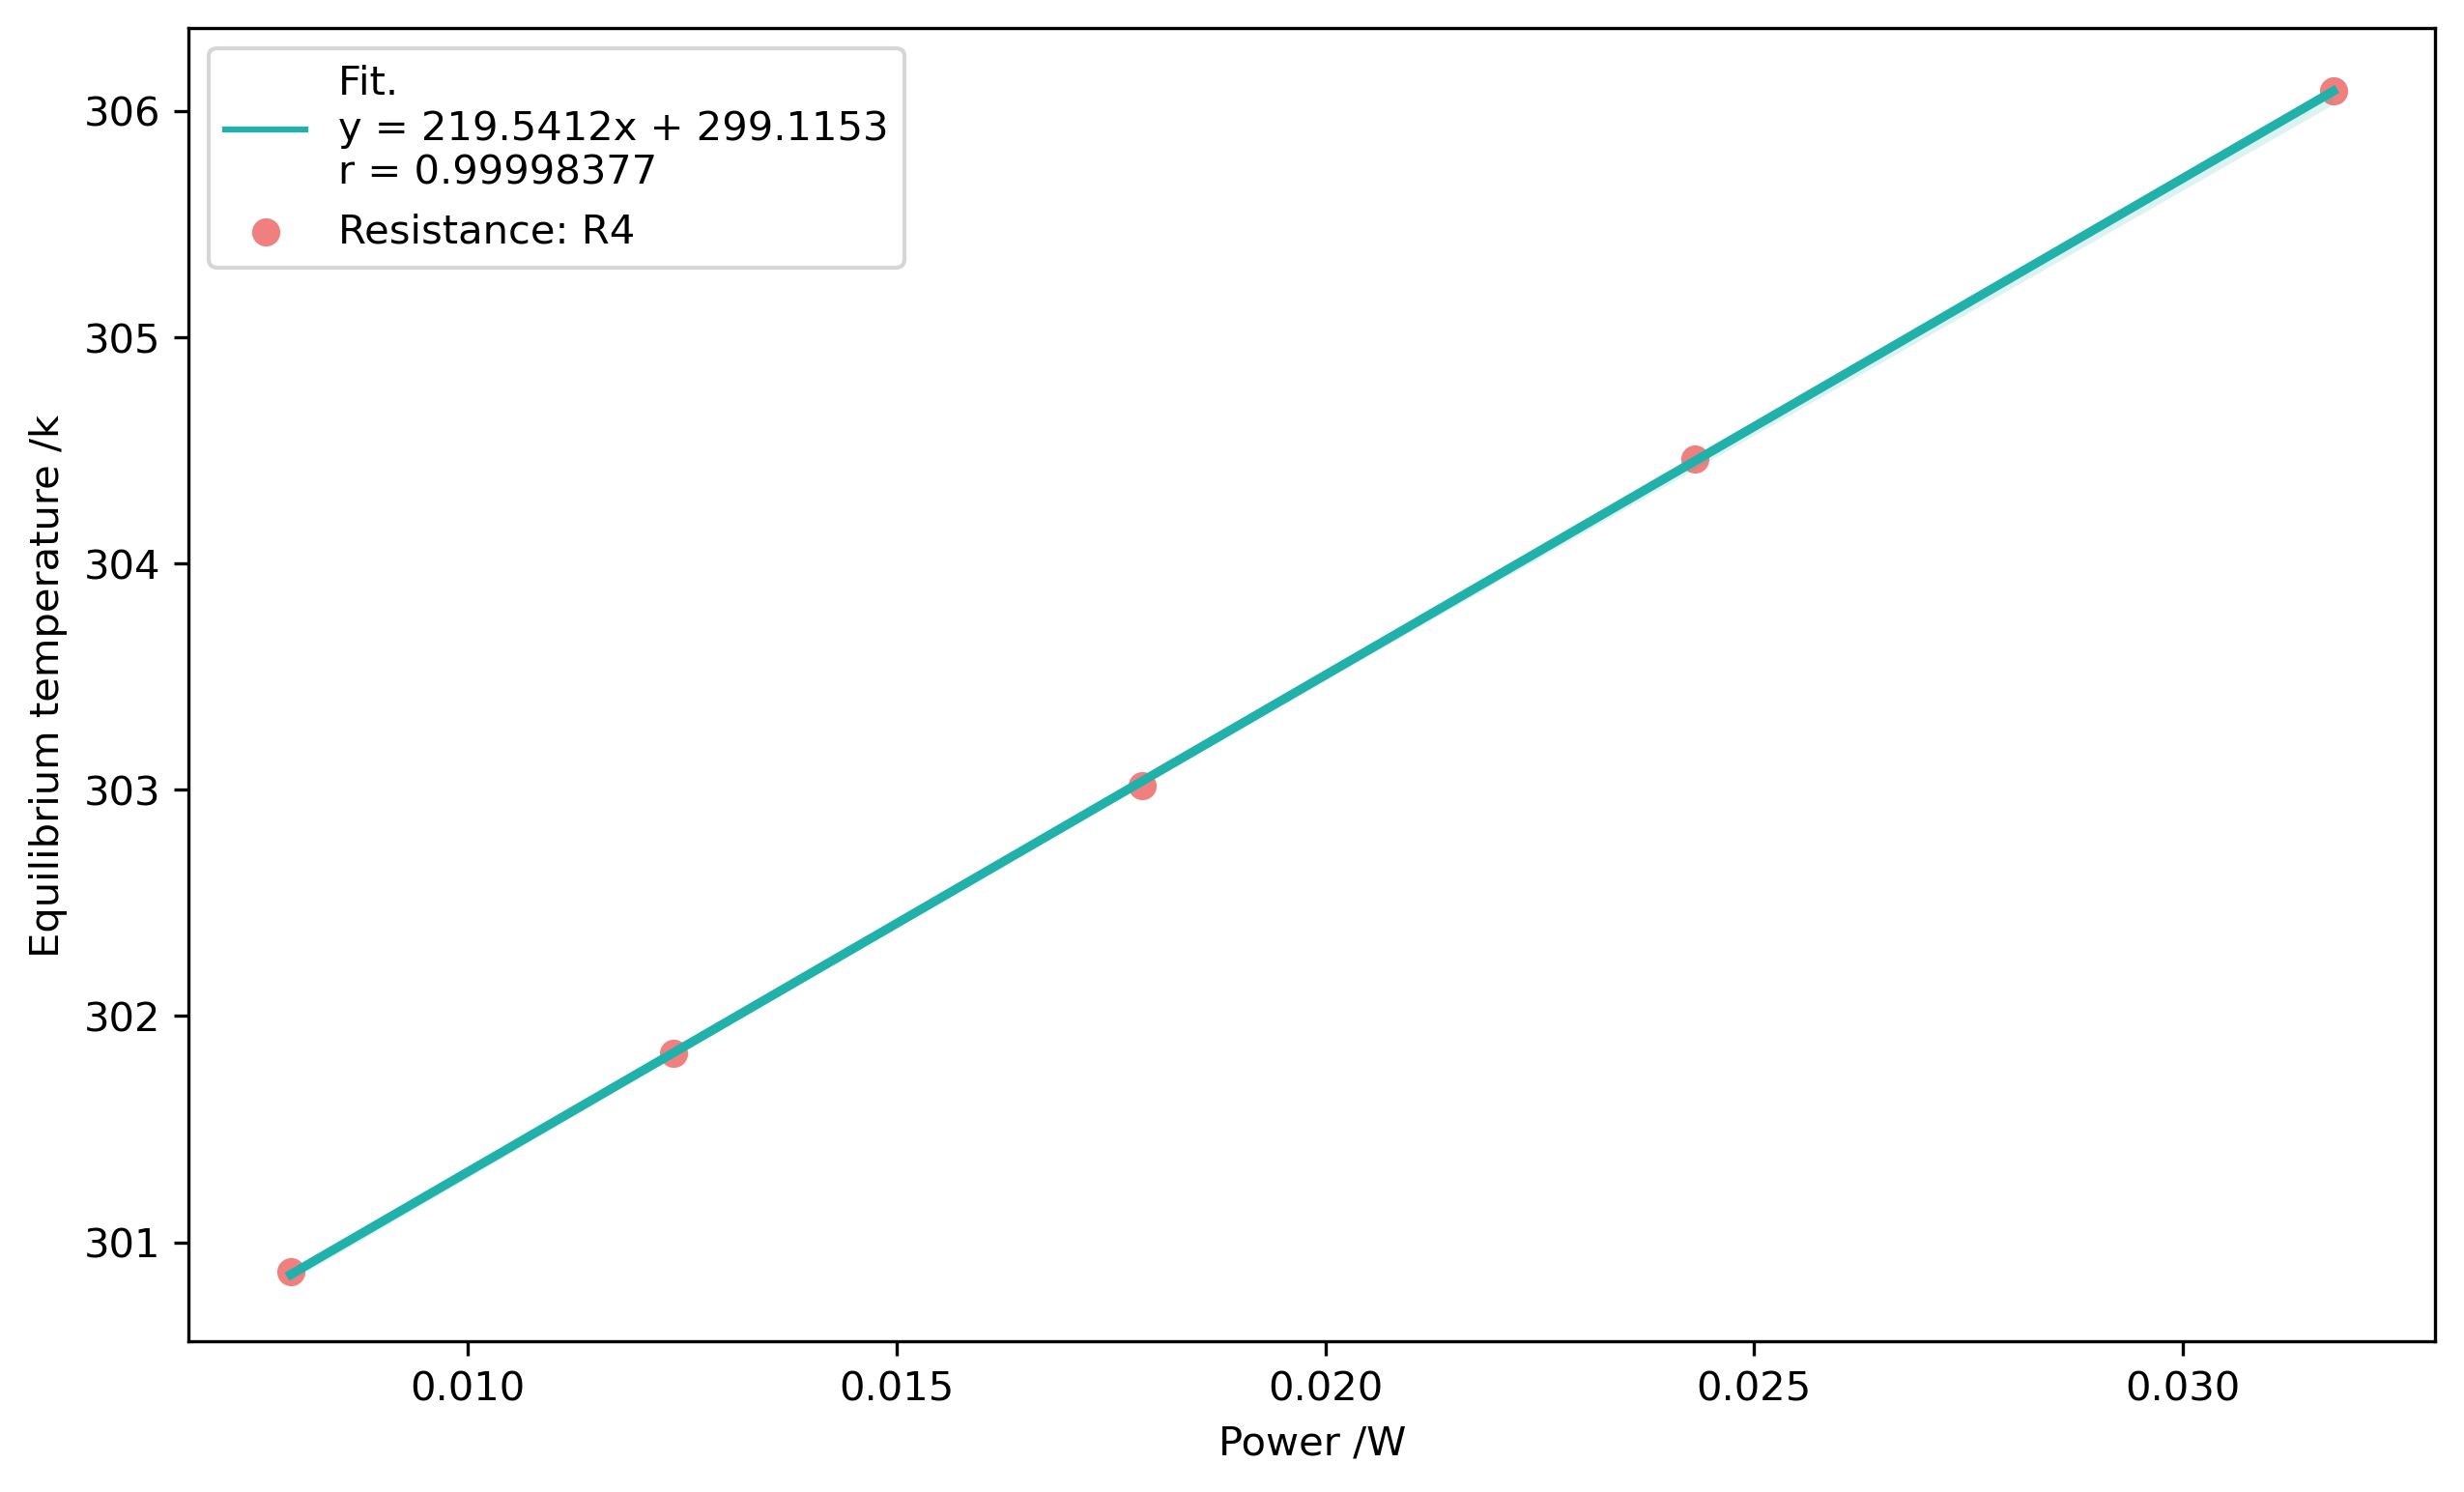
\includegraphics[width=0.3\textwidth]{attachments/fig.1.2.2.4.png}
		}
		\caption{\textbf{Correlation of equilibrium temperature and the heating power, simulation experiments of the ideal model}}
		\label{fig.1.2.2}
	\end{figure*}



	\paragraph{B2. Simulation: The complex model}~
	\newline 
	\indent
	Next, we built the complex resistor thermal model basing on the actual structure of the resistor(Fig. \ref{fig.illus-1.3}) and run the simulation on COMSOL platform.
	The geometric model of the thermal model of the complex resistor thermal model was shown in Fig. \ref{fig.1.3.0}, in which the resistor, 
	which was composed of a copper shell and a ceramic core, was linked in series and embedded in the sponge.
	With different currents provided, the heating curves and the following cooling curves were obtained(Fig. \ref{fig.1.3.1}),
	and the correlation of the equilibrium temperatures of each resistor and the heating powers were shown in Fig. \ref{fig.1.3.2}.

	Results show that the equilibrium temperature was directly proportional to the resist value, which is consistent with the real-world experiment and the previous simulation model.

	\begin{figure*}[htbp]
		\centering
		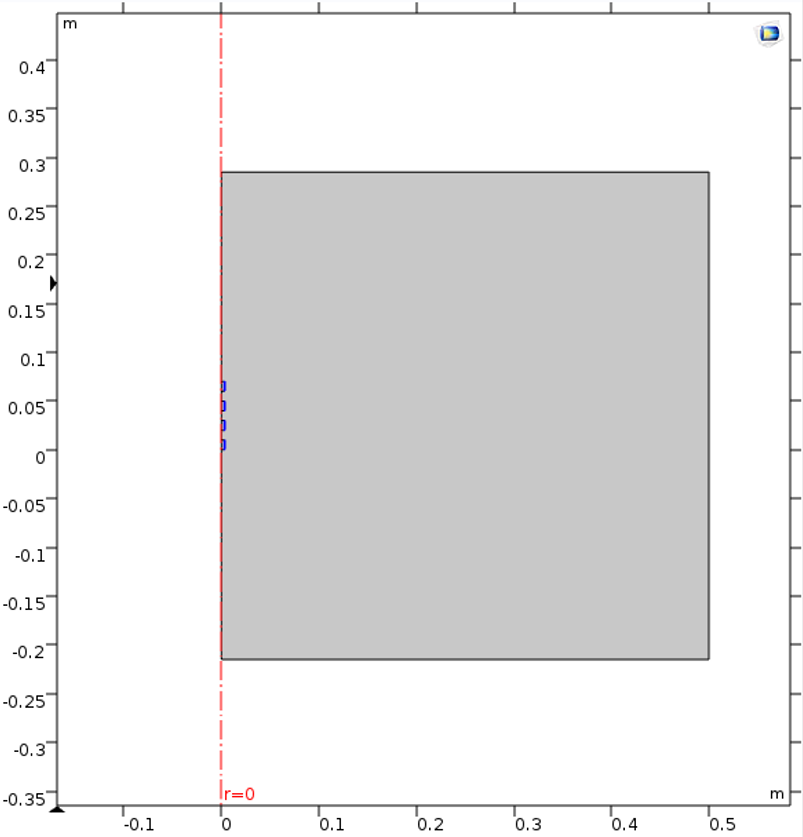
\includegraphics[width=0.3\textwidth]{attachments/fig.1.3.0.png}
		\caption{\textbf{The geometric model of the complex resistor model}}
		\label{fig.1.3.0}
	\end{figure*}
	
	\begin{figure*}[htbp]
		\centering
		\subfloat[$I=0.020A$]{\label{fig.1.3.1.1}
		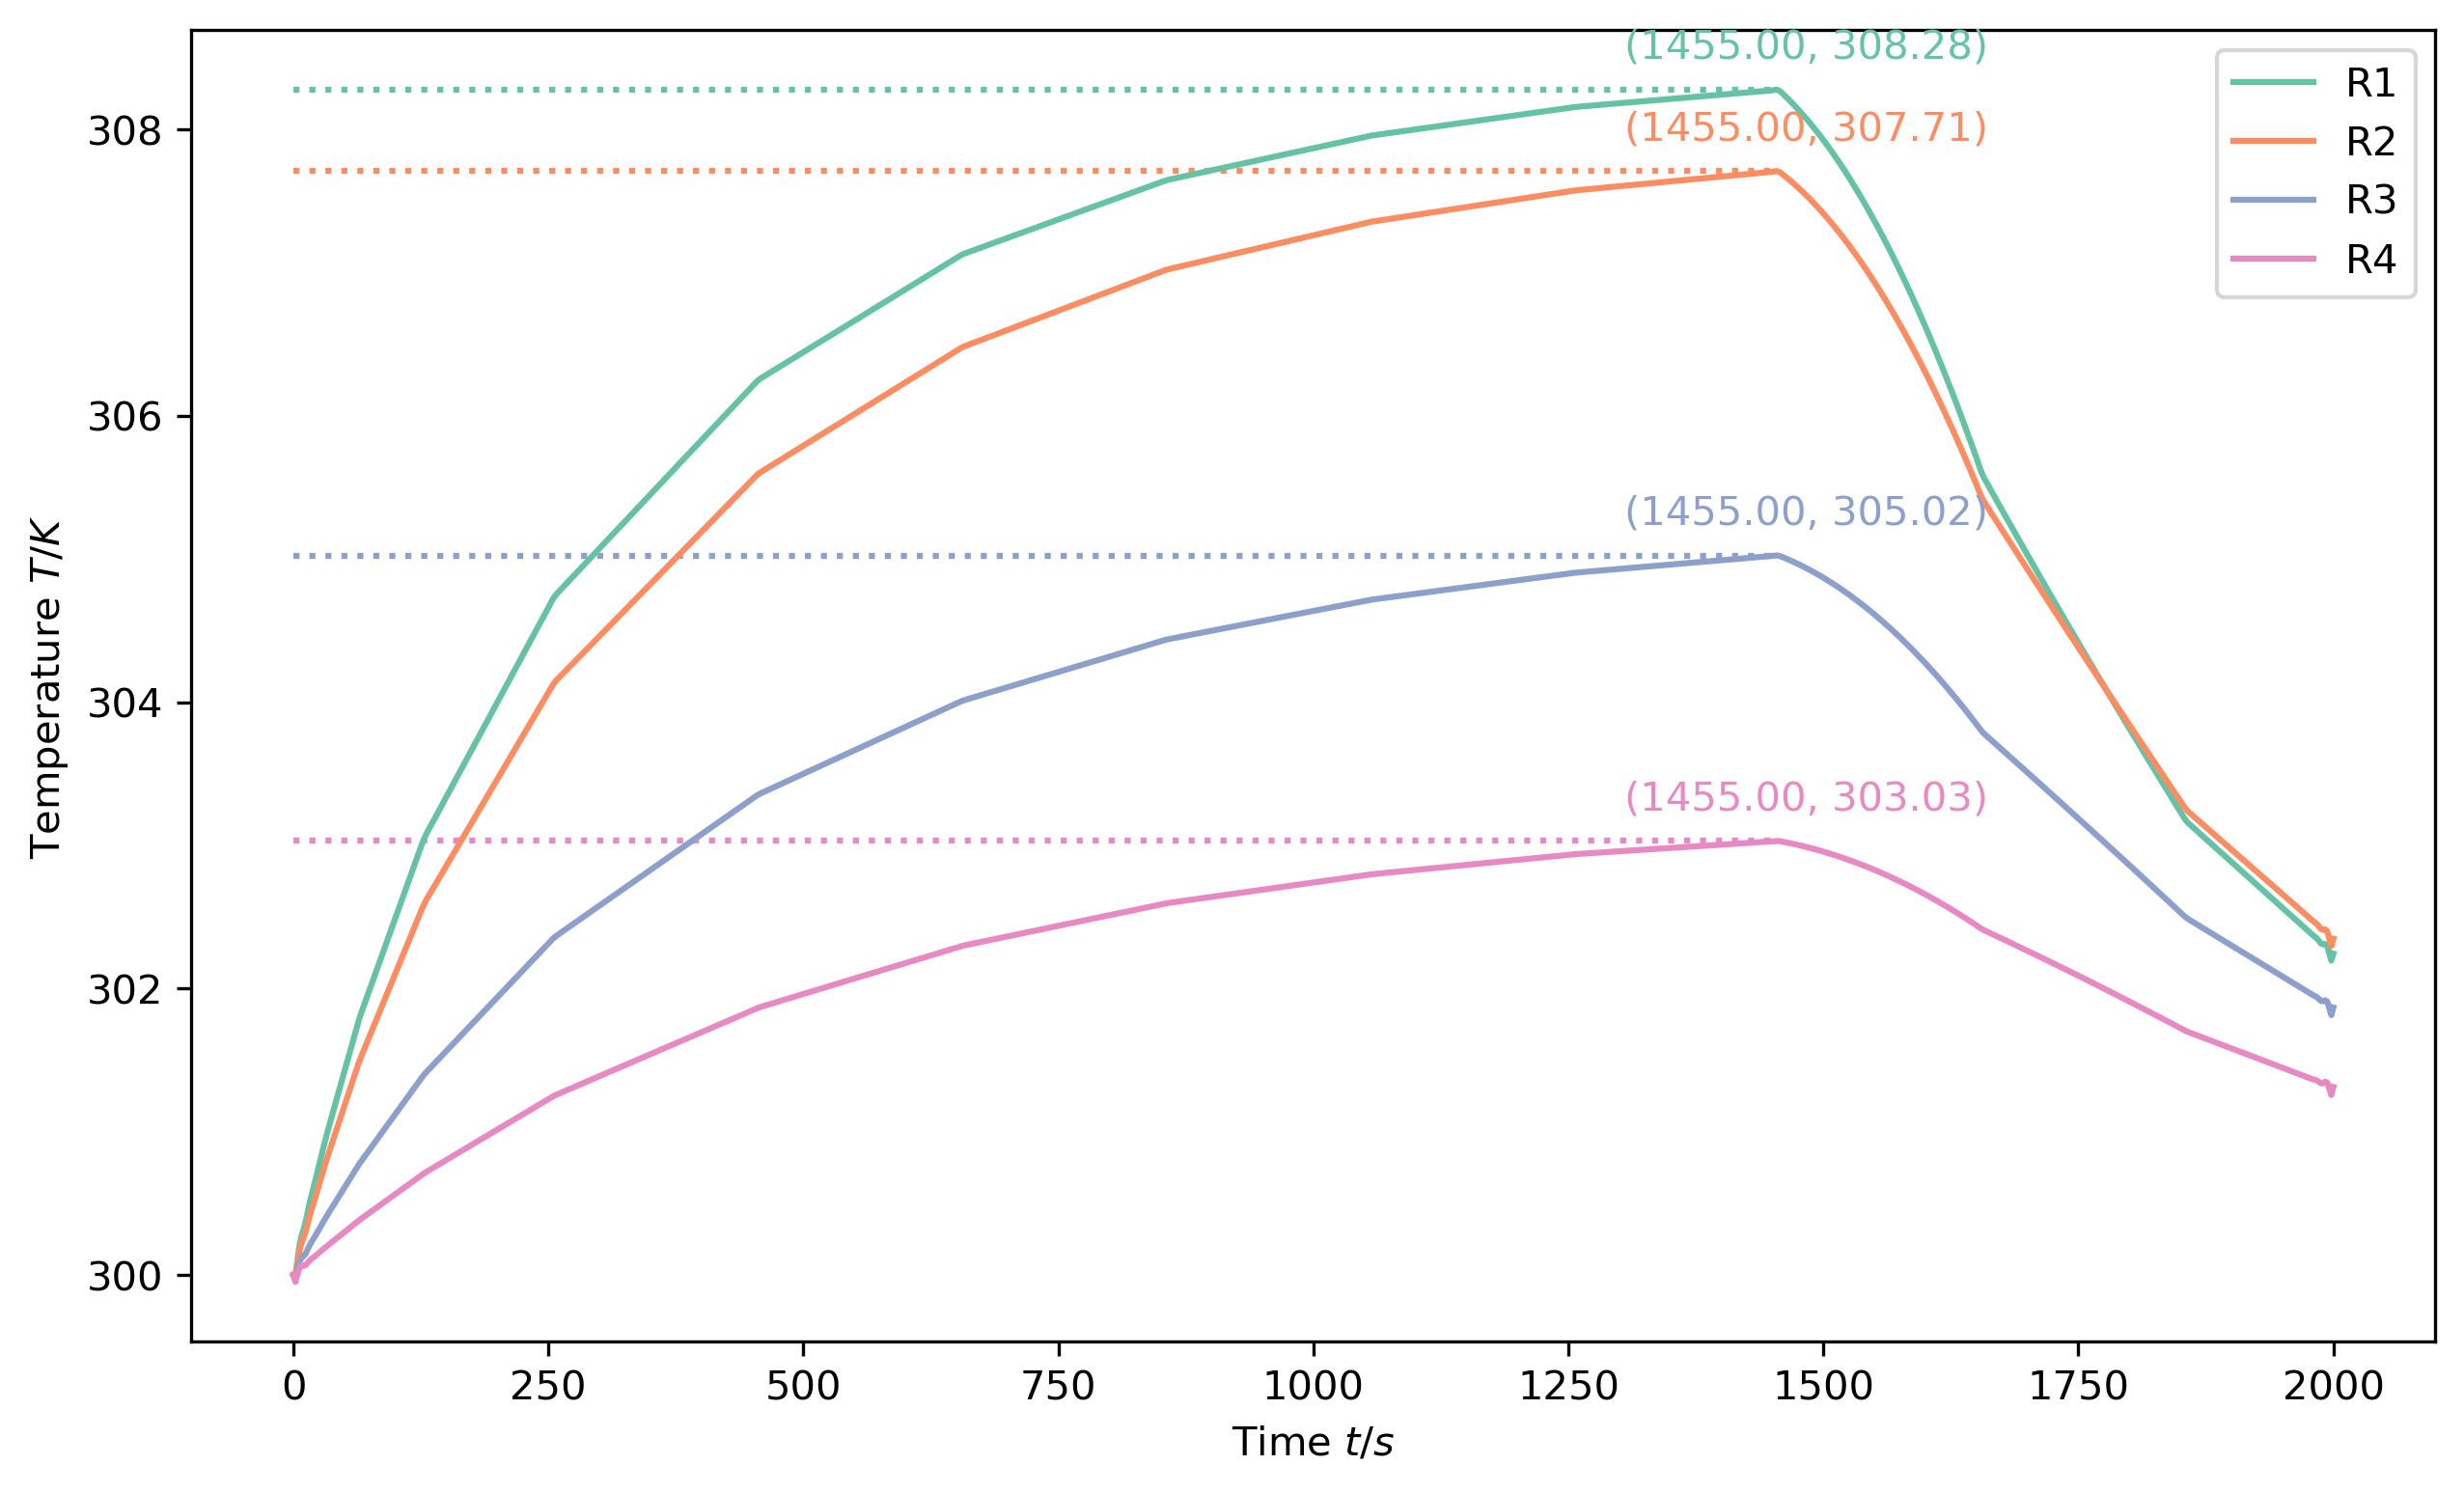
\includegraphics[width=0.3\textwidth]{attachments/fig.1.3.1.1.png}
		}		
		\subfloat[$I=0.025A$]{\label{fig.1.3.1.2}
		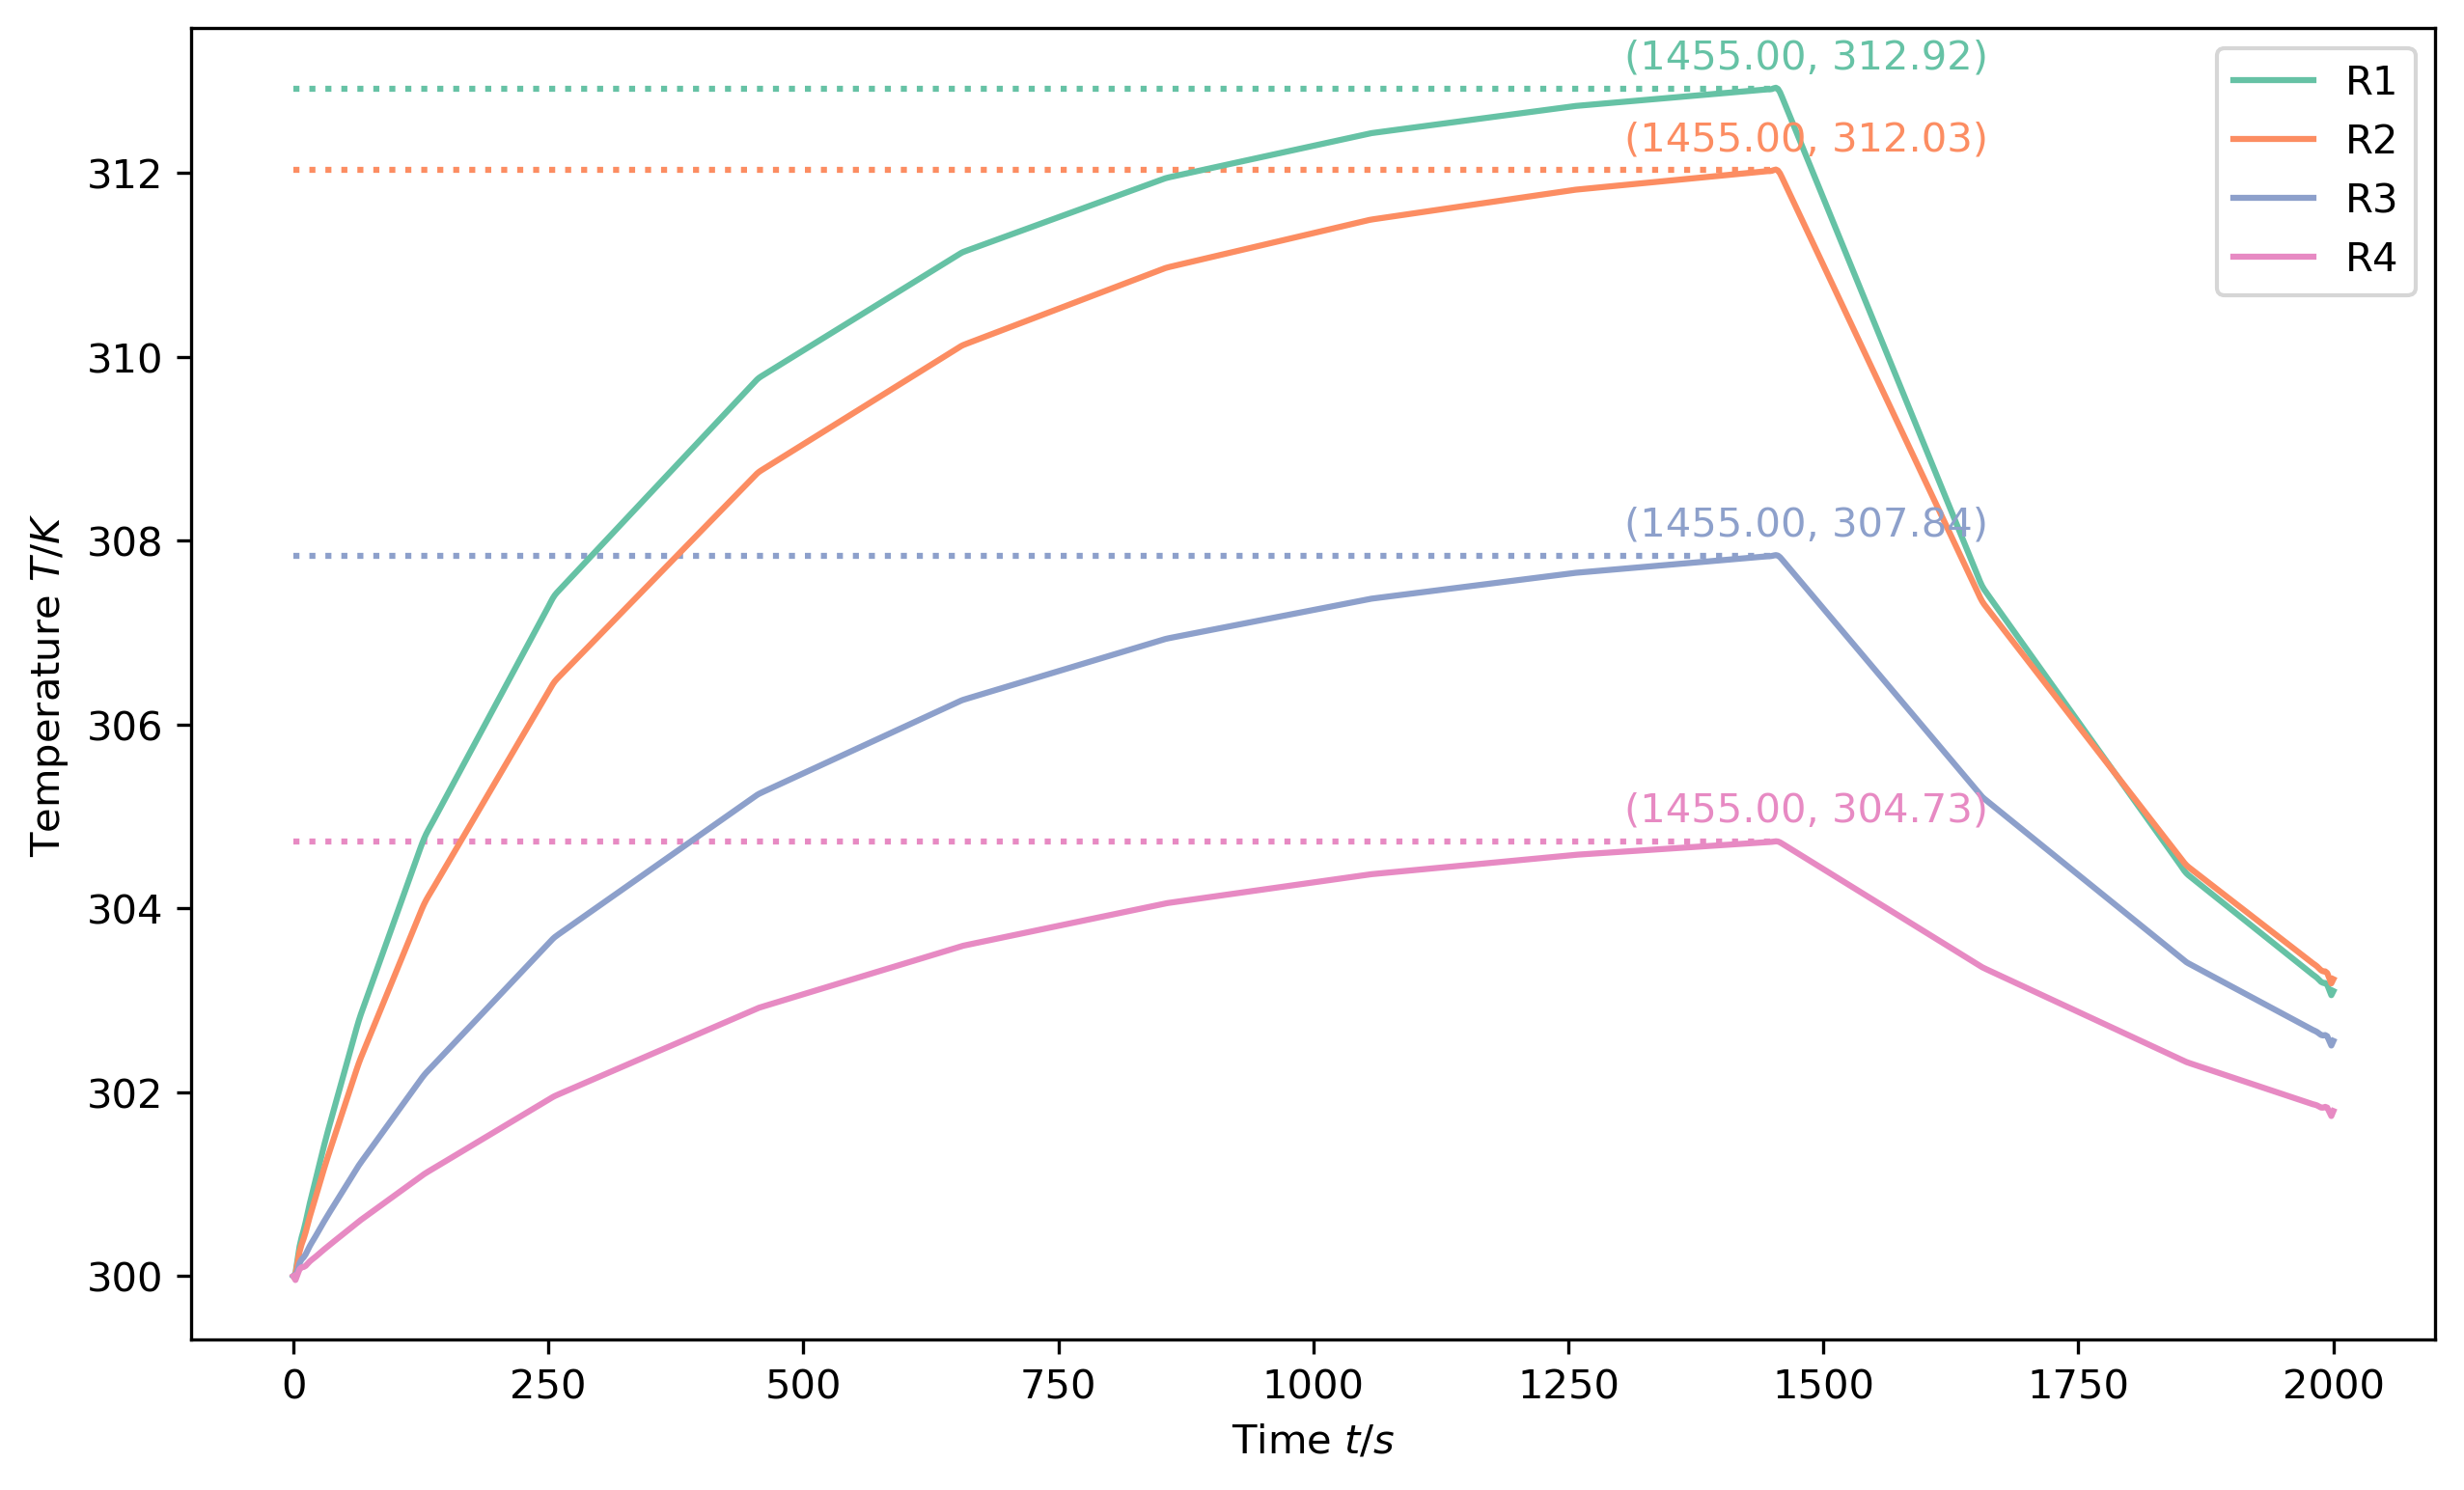
\includegraphics[width=0.3\textwidth]{attachments/fig.1.3.1.2.png}
		}

		\subfloat[$I=0.030A$]{\label{fig.1.3.1.3}
		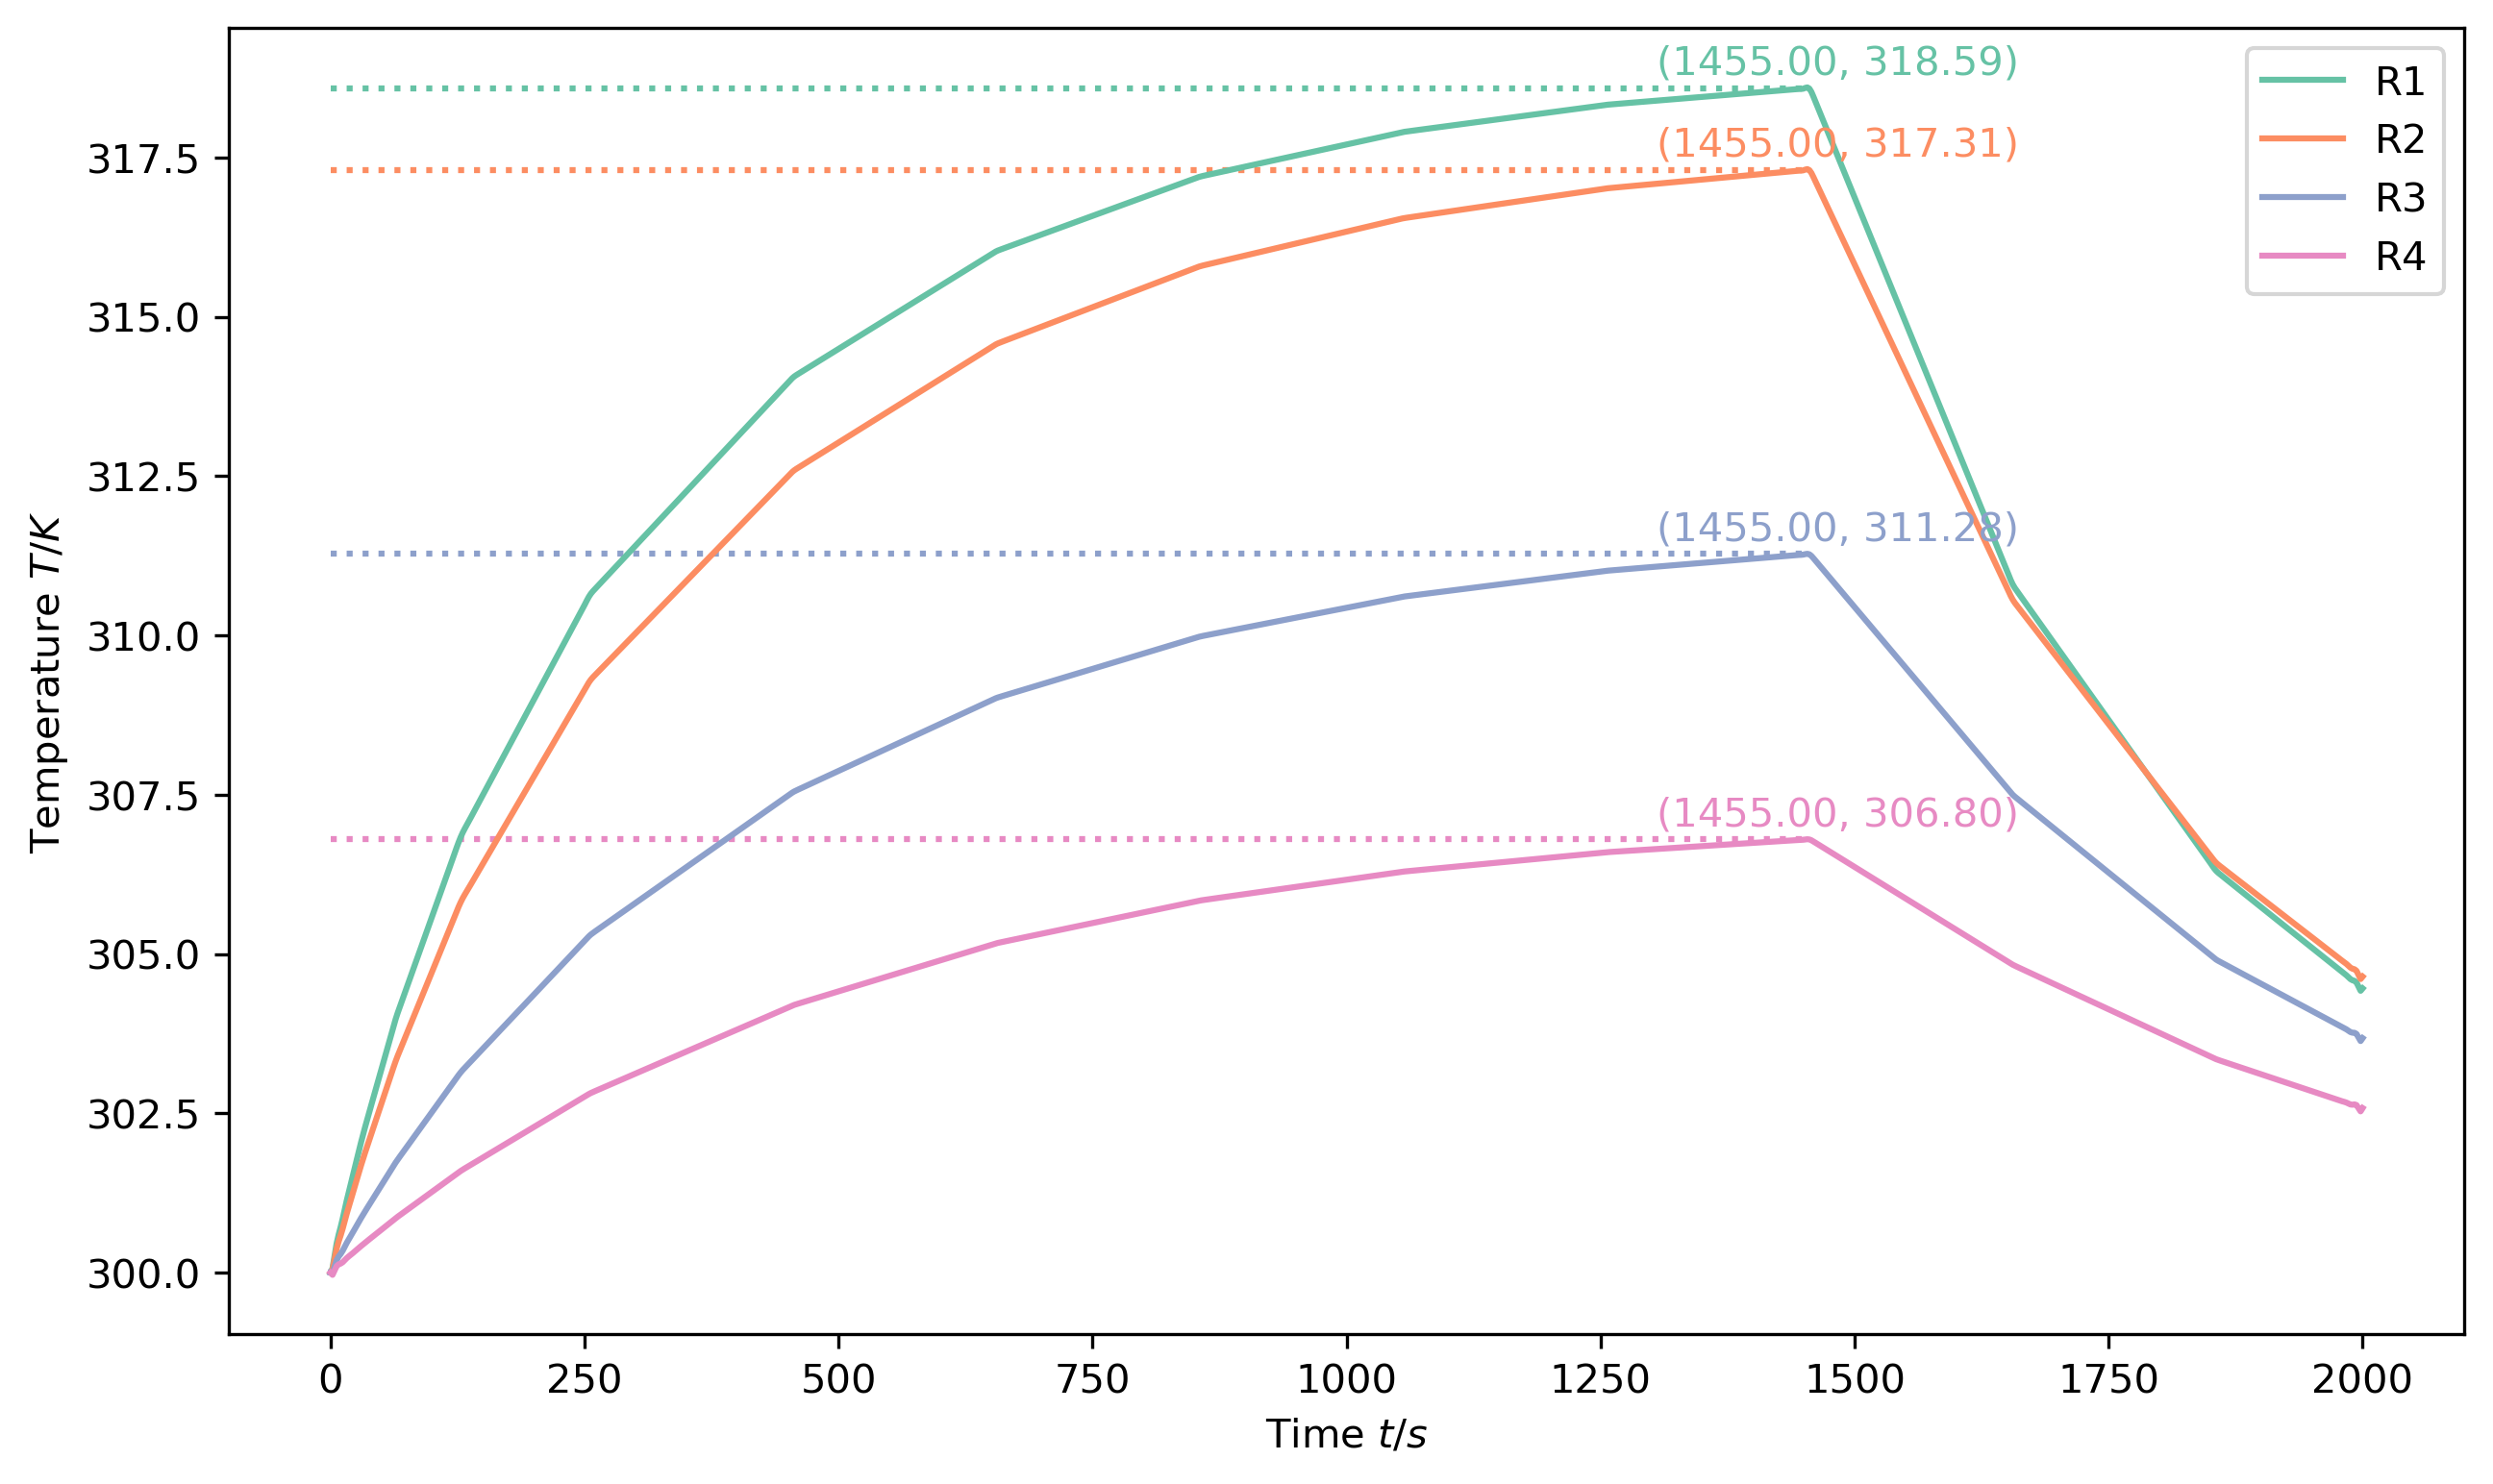
\includegraphics[width=0.3\textwidth]{attachments/fig.1.3.1.3.png}
		}
		\subfloat[$I=0.035A$]{\label{fig.1.3.1.4}
		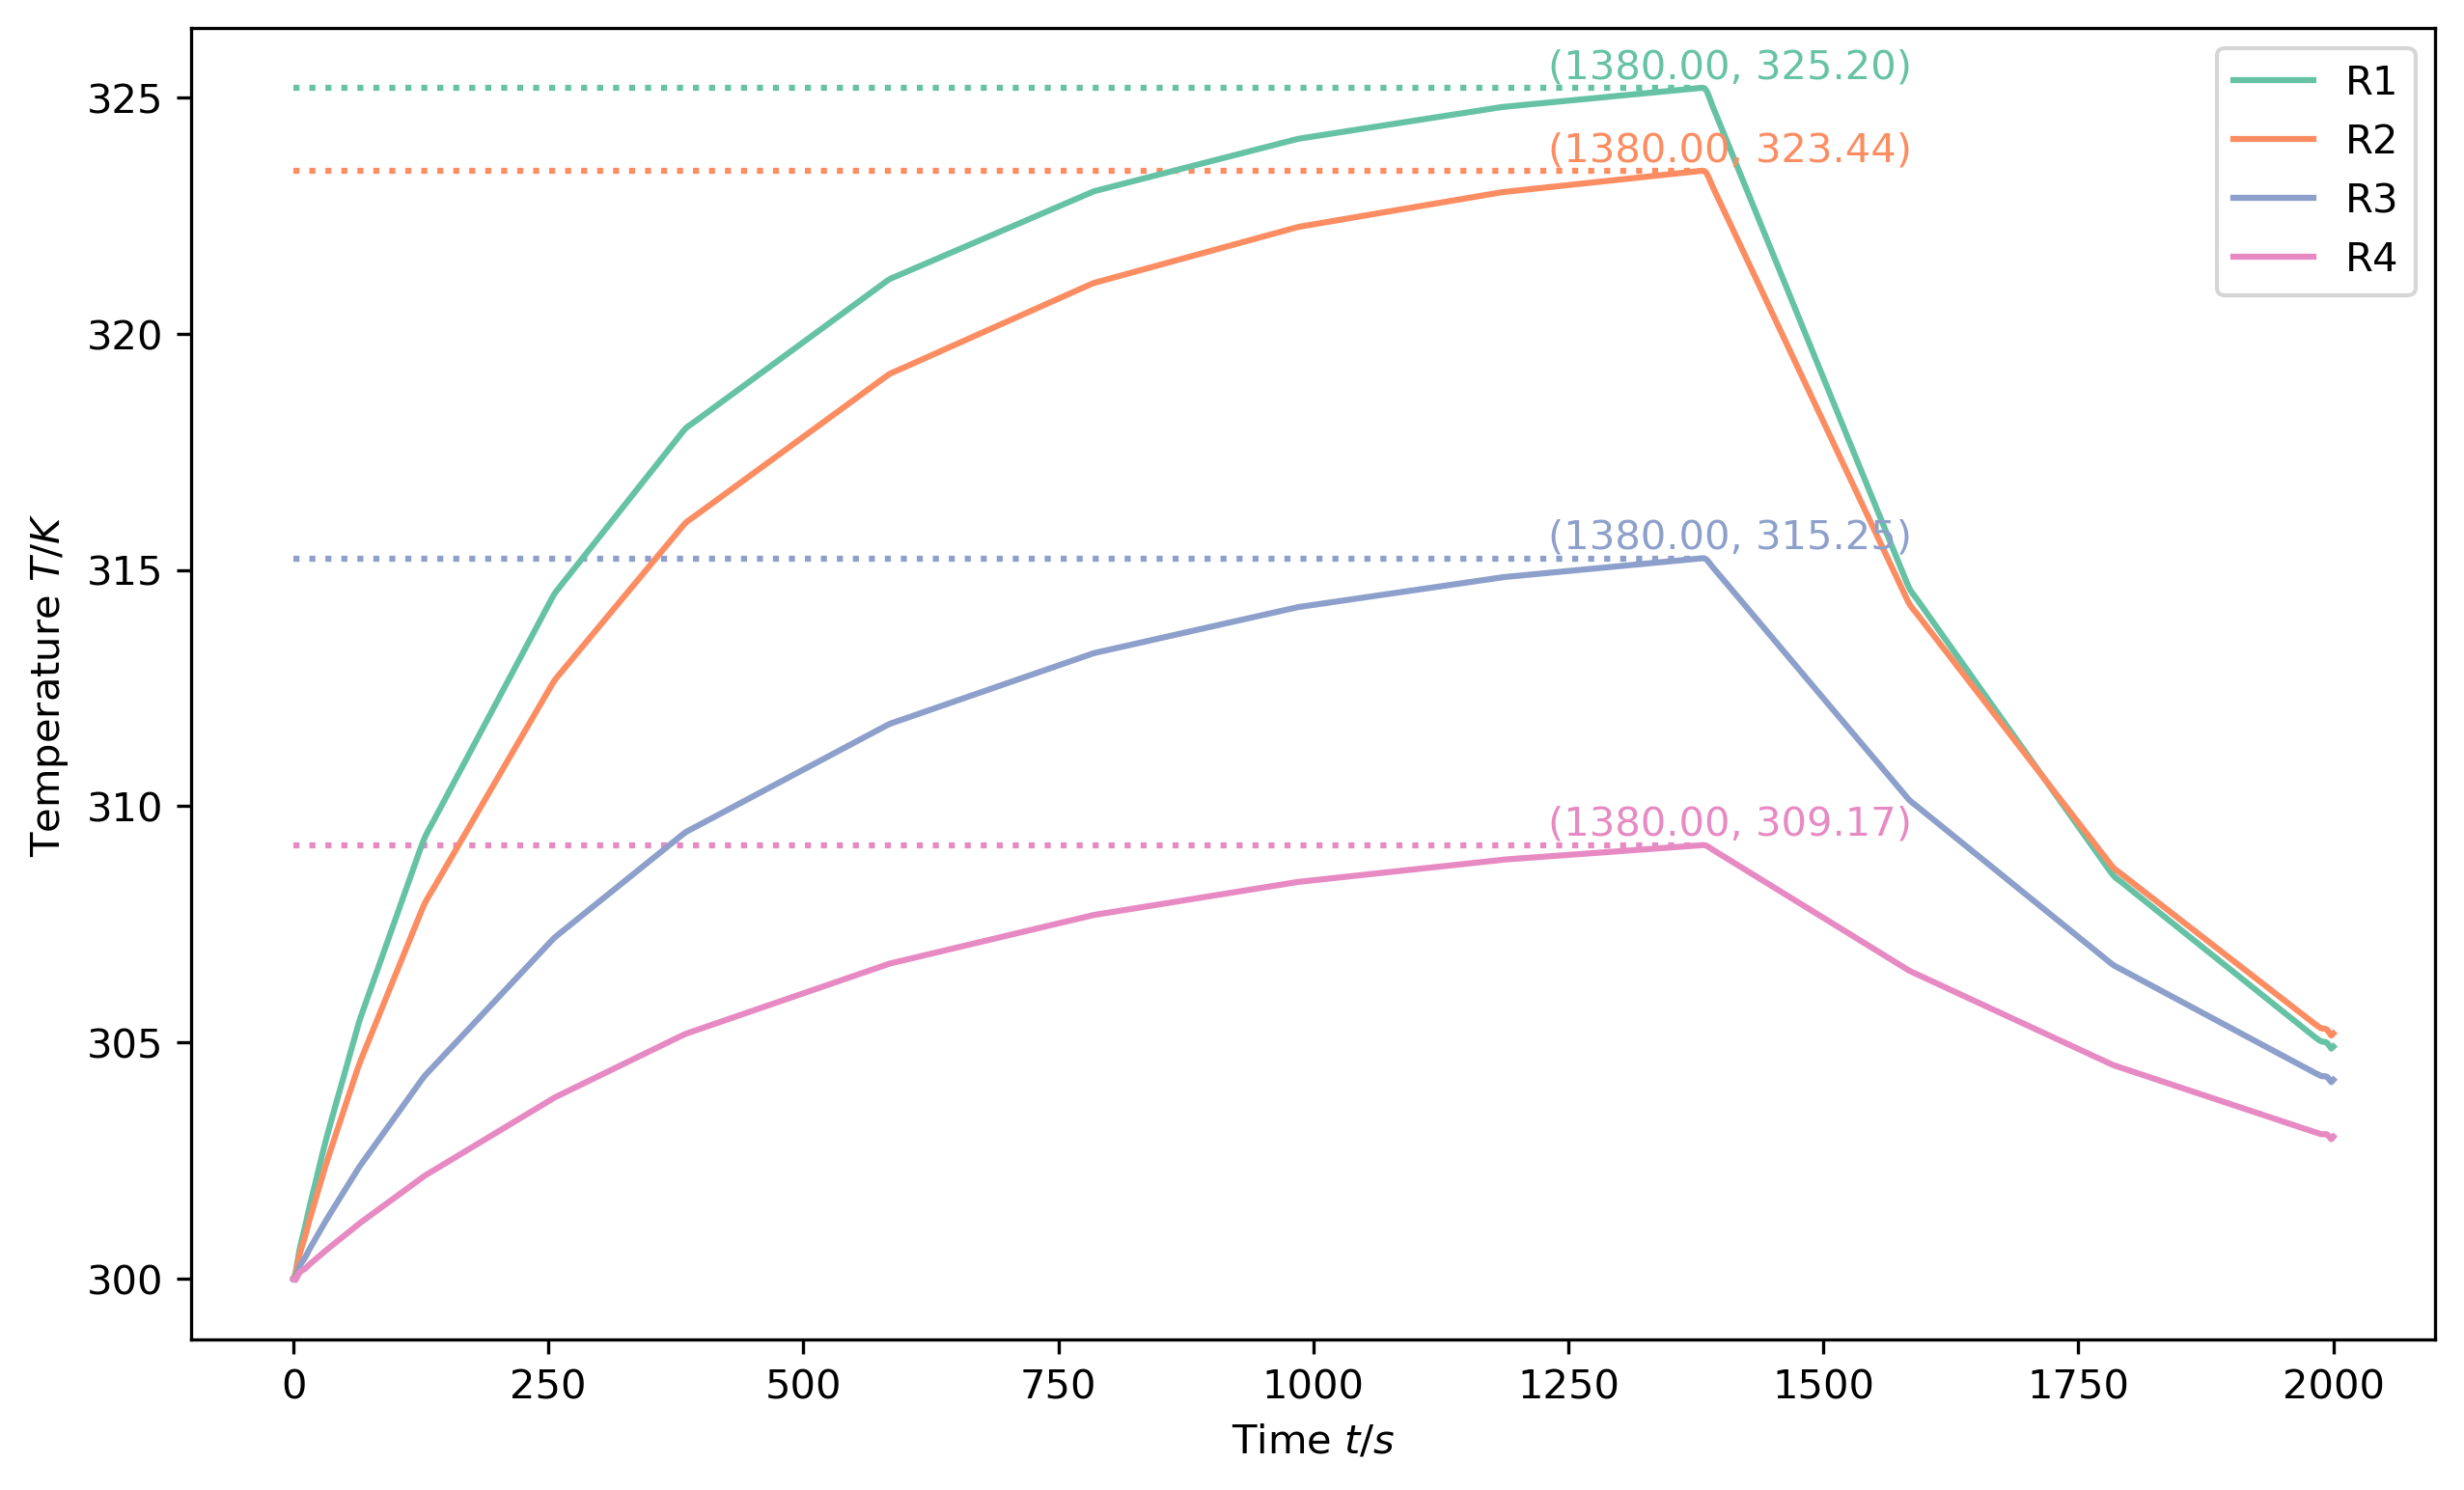
\includegraphics[width=0.3\textwidth]{attachments/fig.1.3.1.4.png}
		}
		\subfloat[$I=0.040A$]{\label{fig.1.3.1.5}
		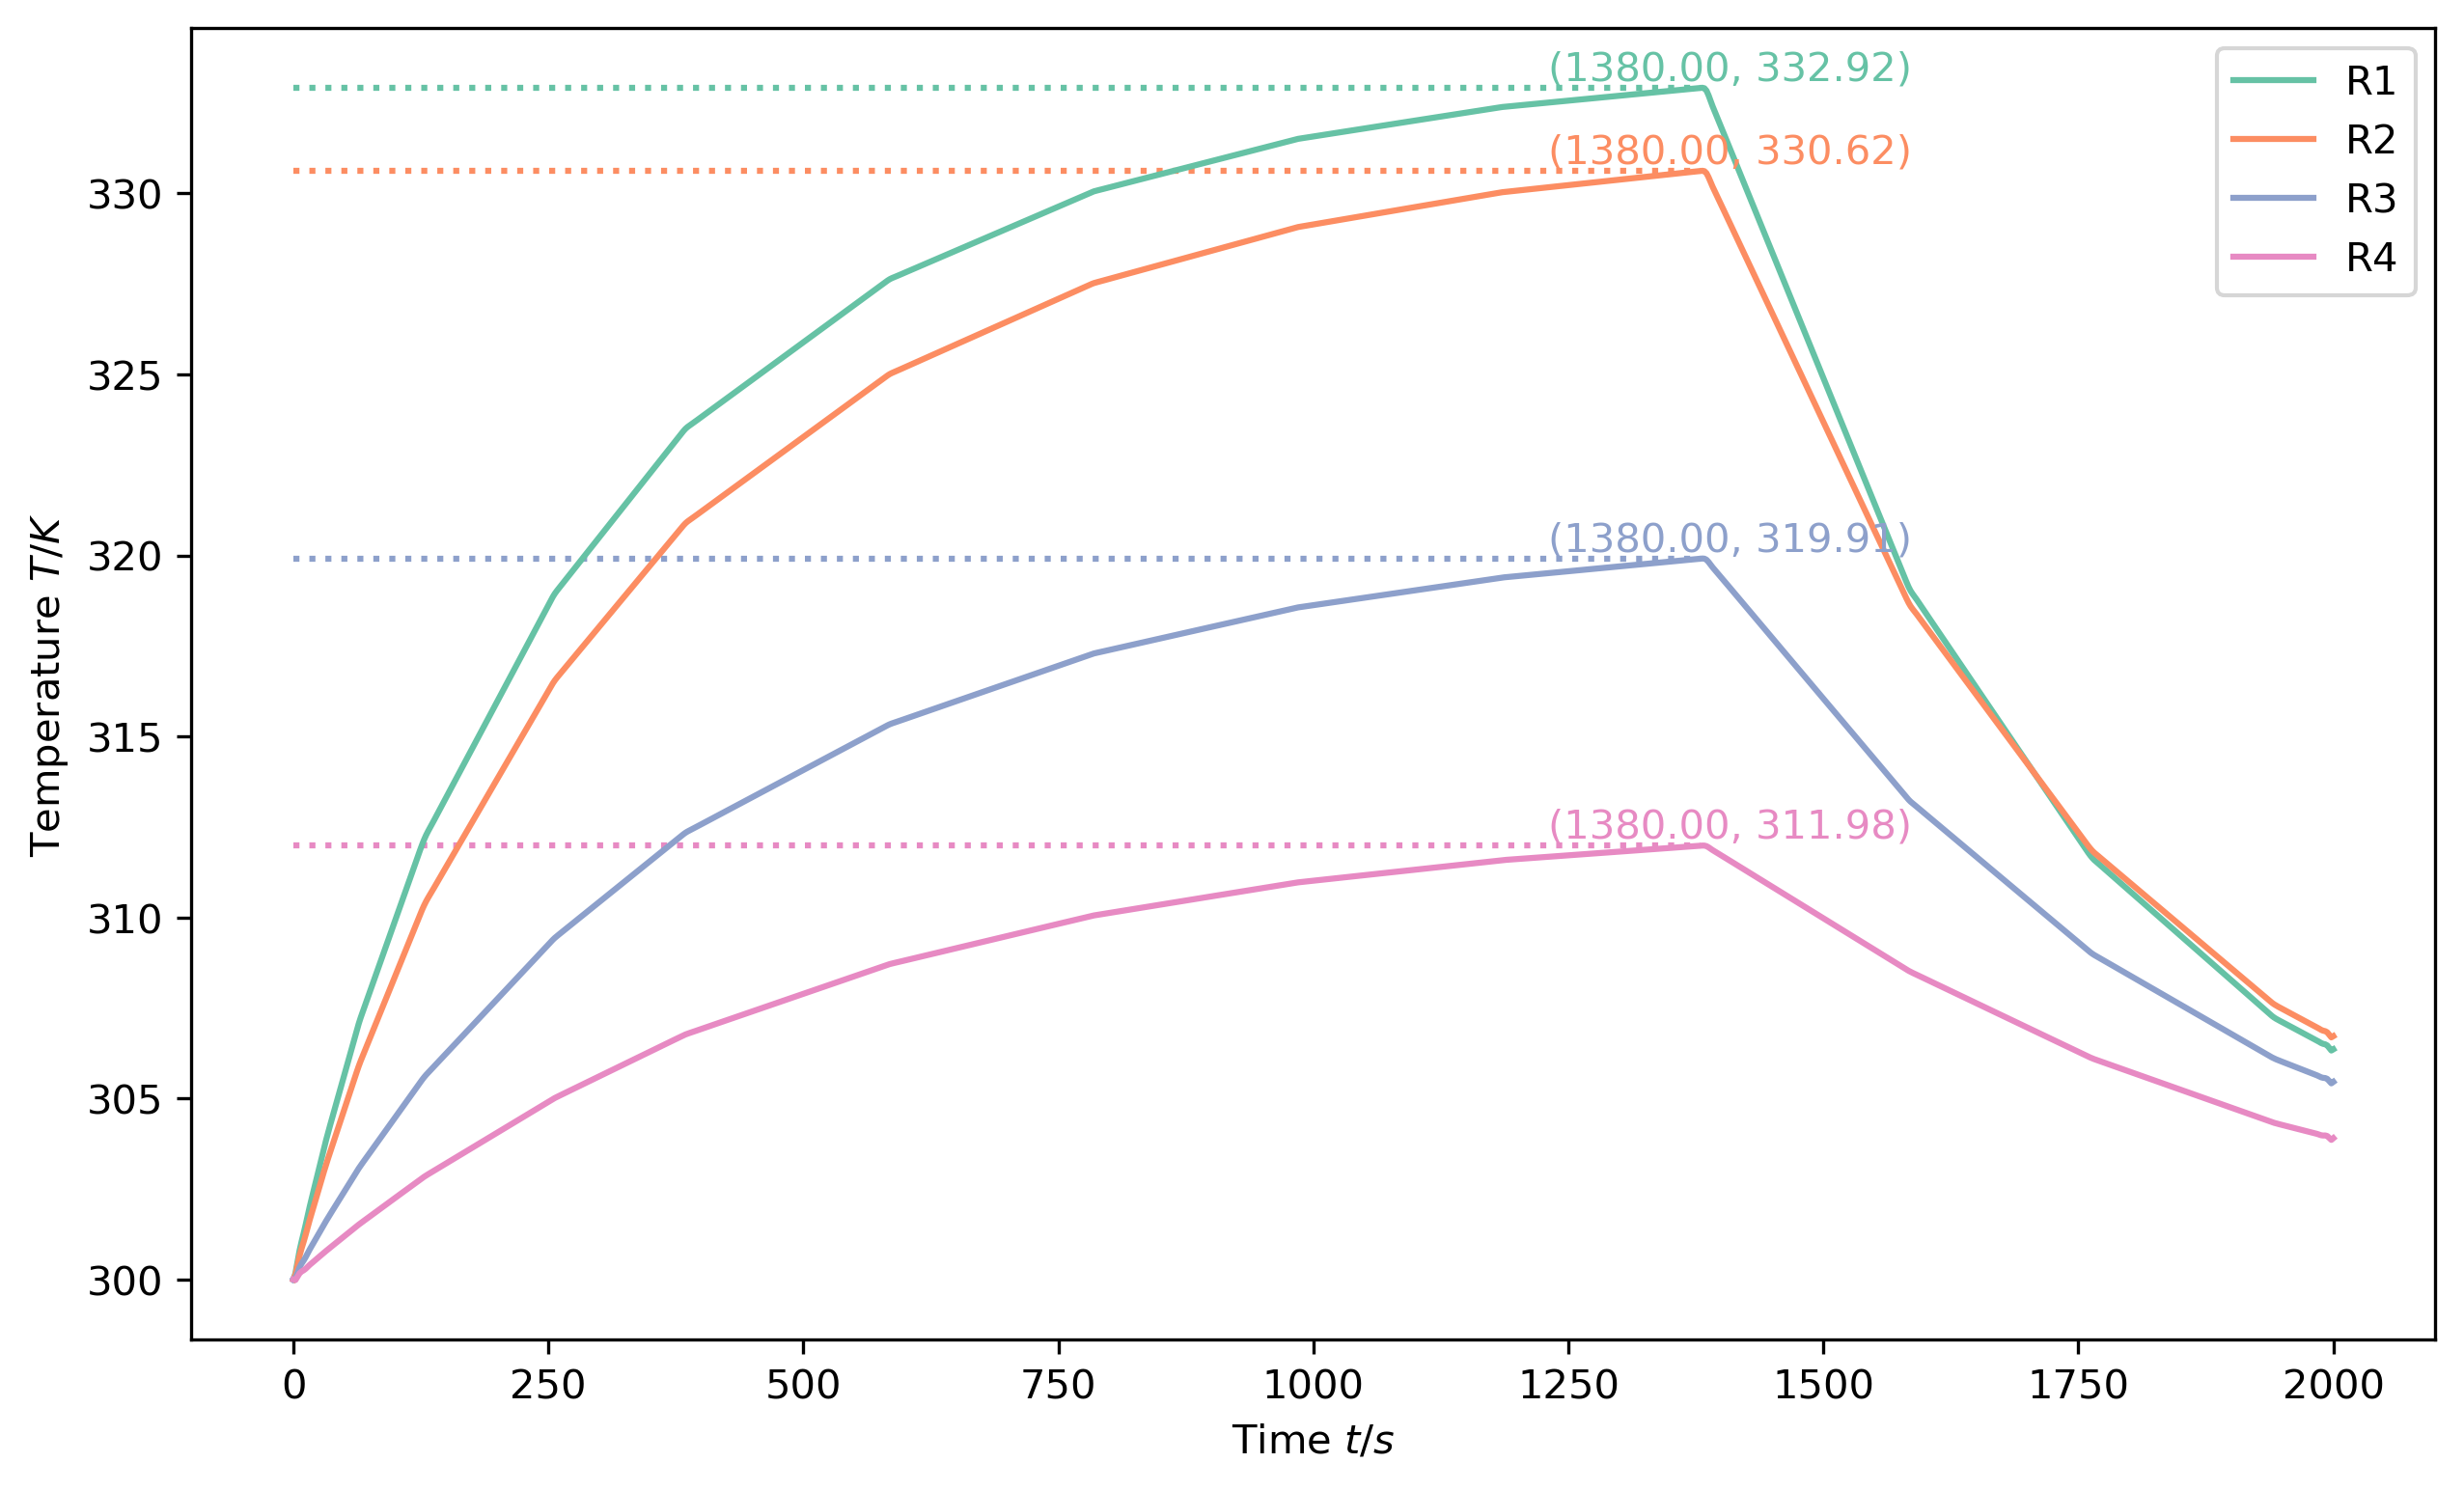
\includegraphics[width=0.3\textwidth]{attachments/fig.1.3.1.5.png}
		}
		\caption{\textbf{Heating and cooling curves of the series resistors under different currents, simulation experiments of the complex model}}
		\label{fig.1.3.1}
	\end{figure*}

	\begin{figure*}[htbp]
		\centering
		\subfloat[$R_1 = 100.00 \Omega$]{\label{fig.1.3.2.1}
		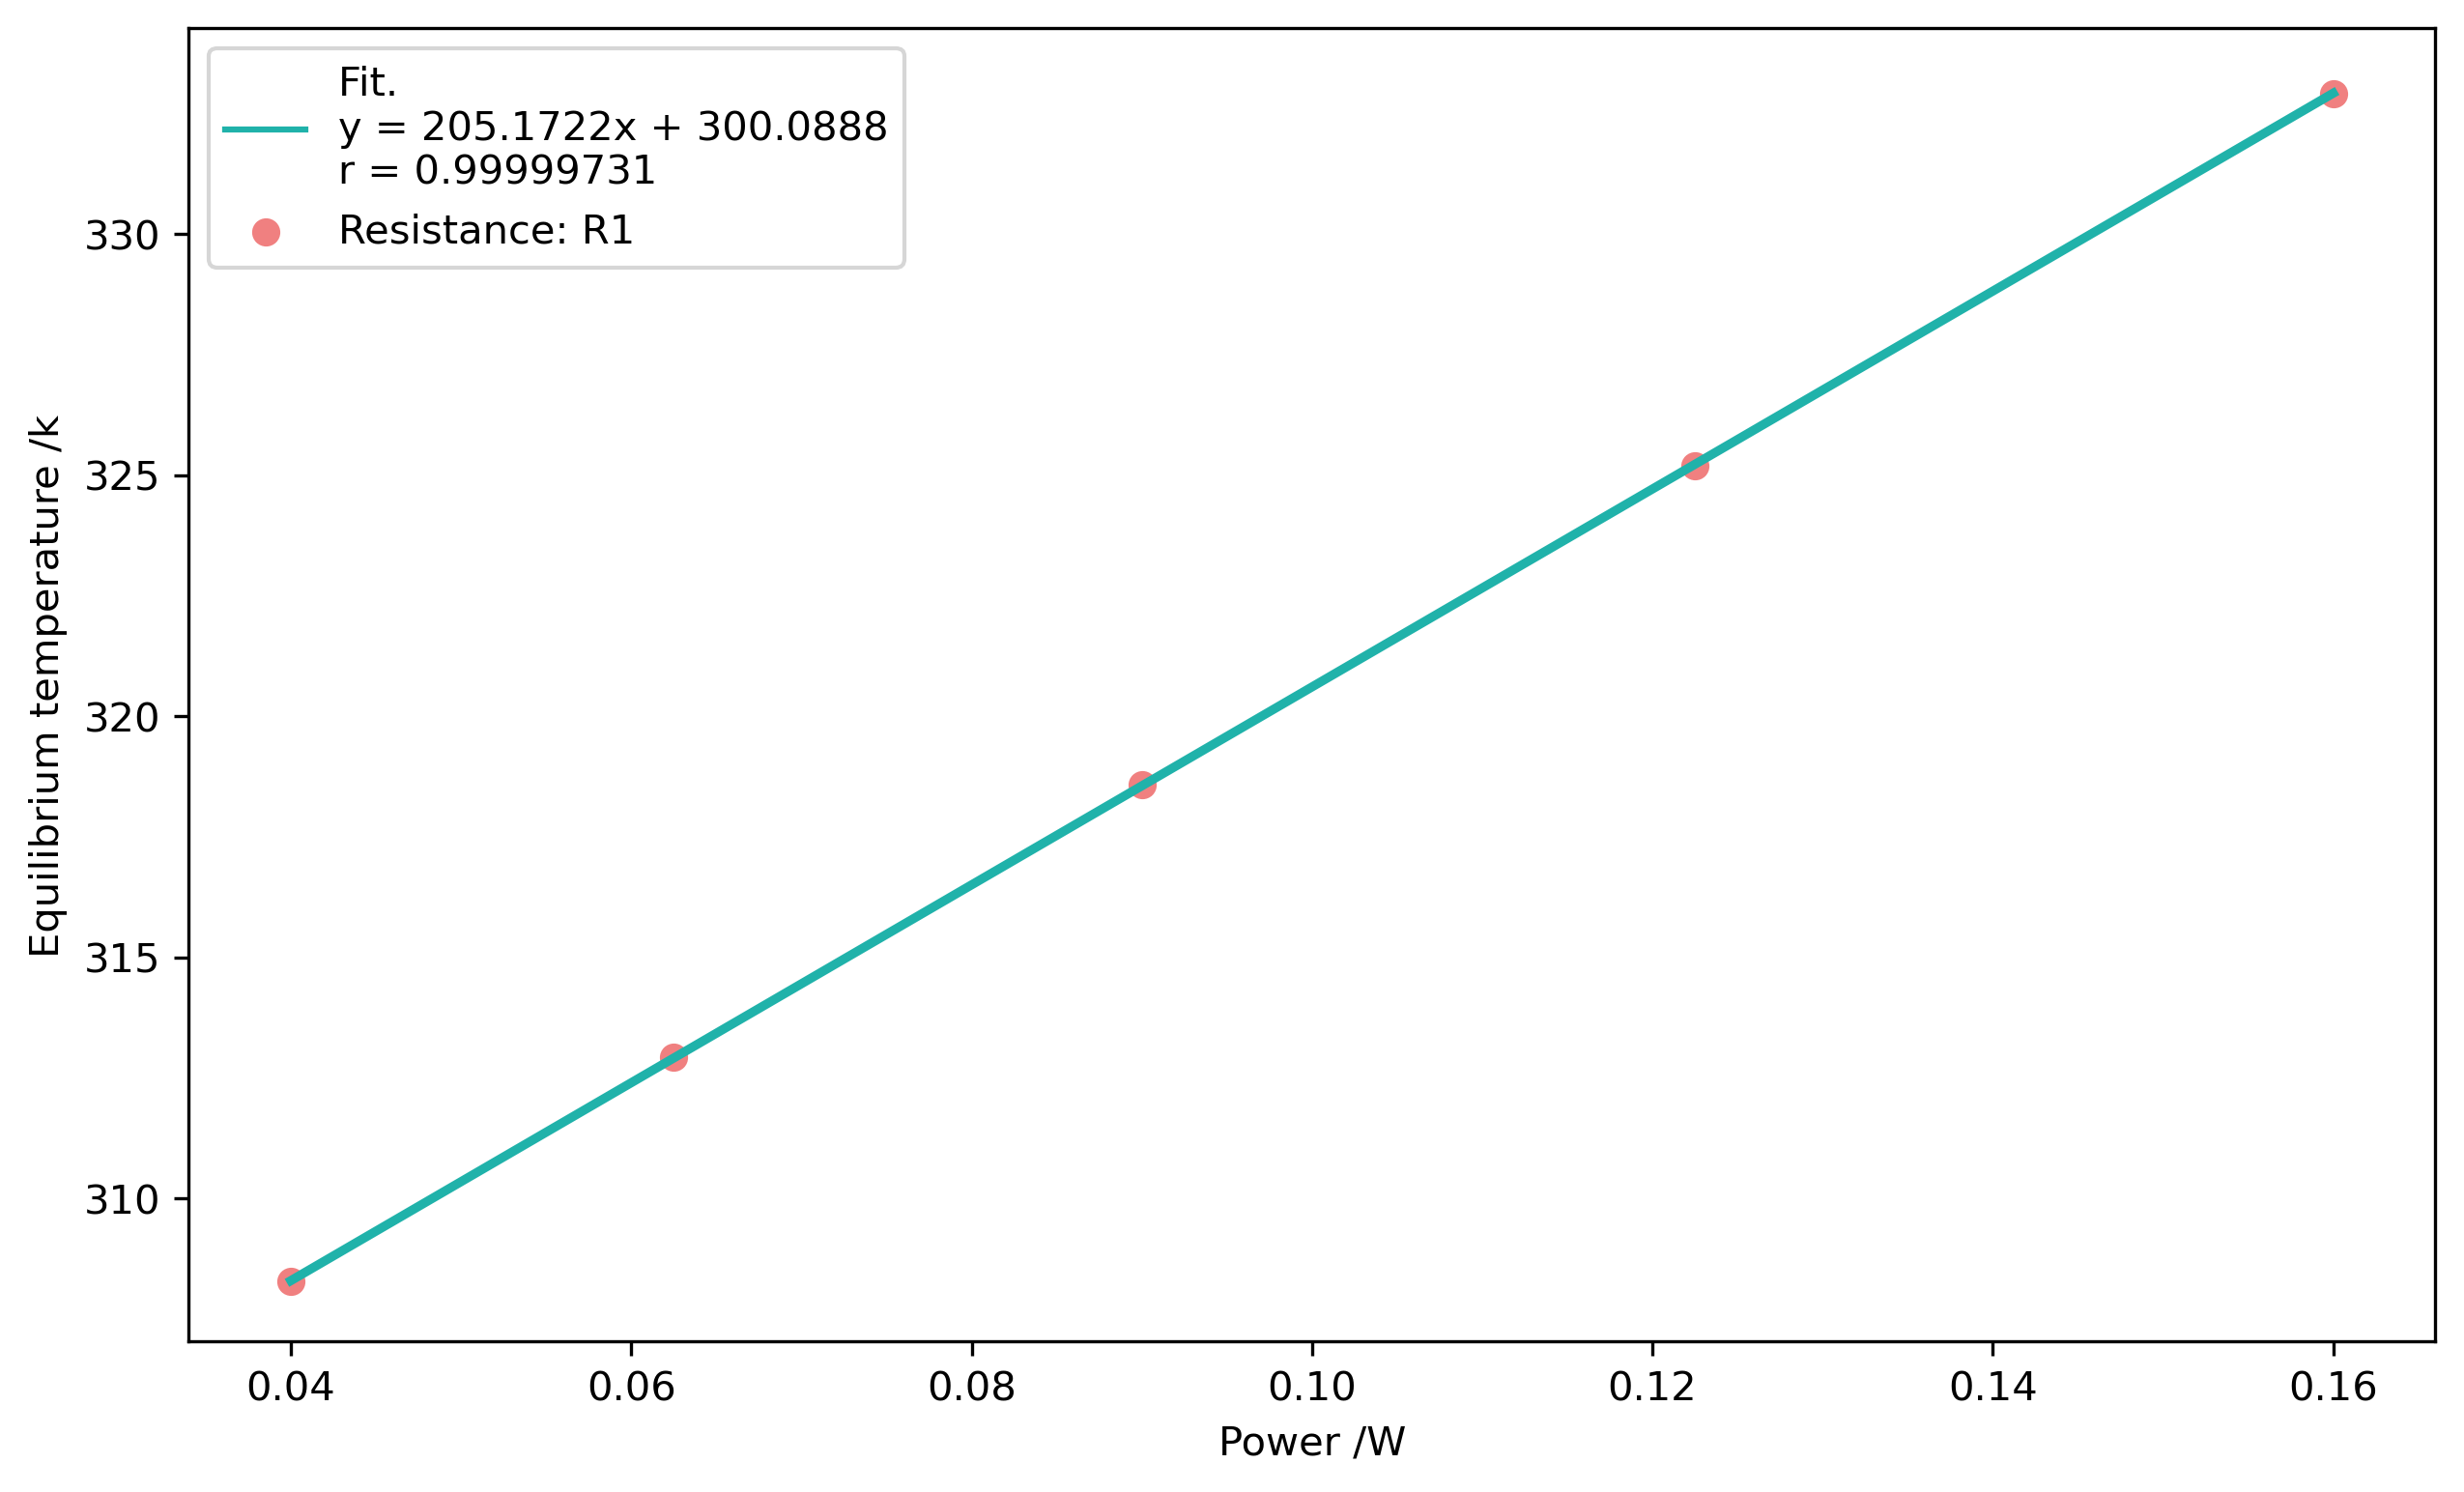
\includegraphics[width=0.3\textwidth]{attachments/fig.1.3.2.1.png}
		}		
		\subfloat[$R_2 = 81.588 \Omega$]{\label{fig.1.3.2.2}
		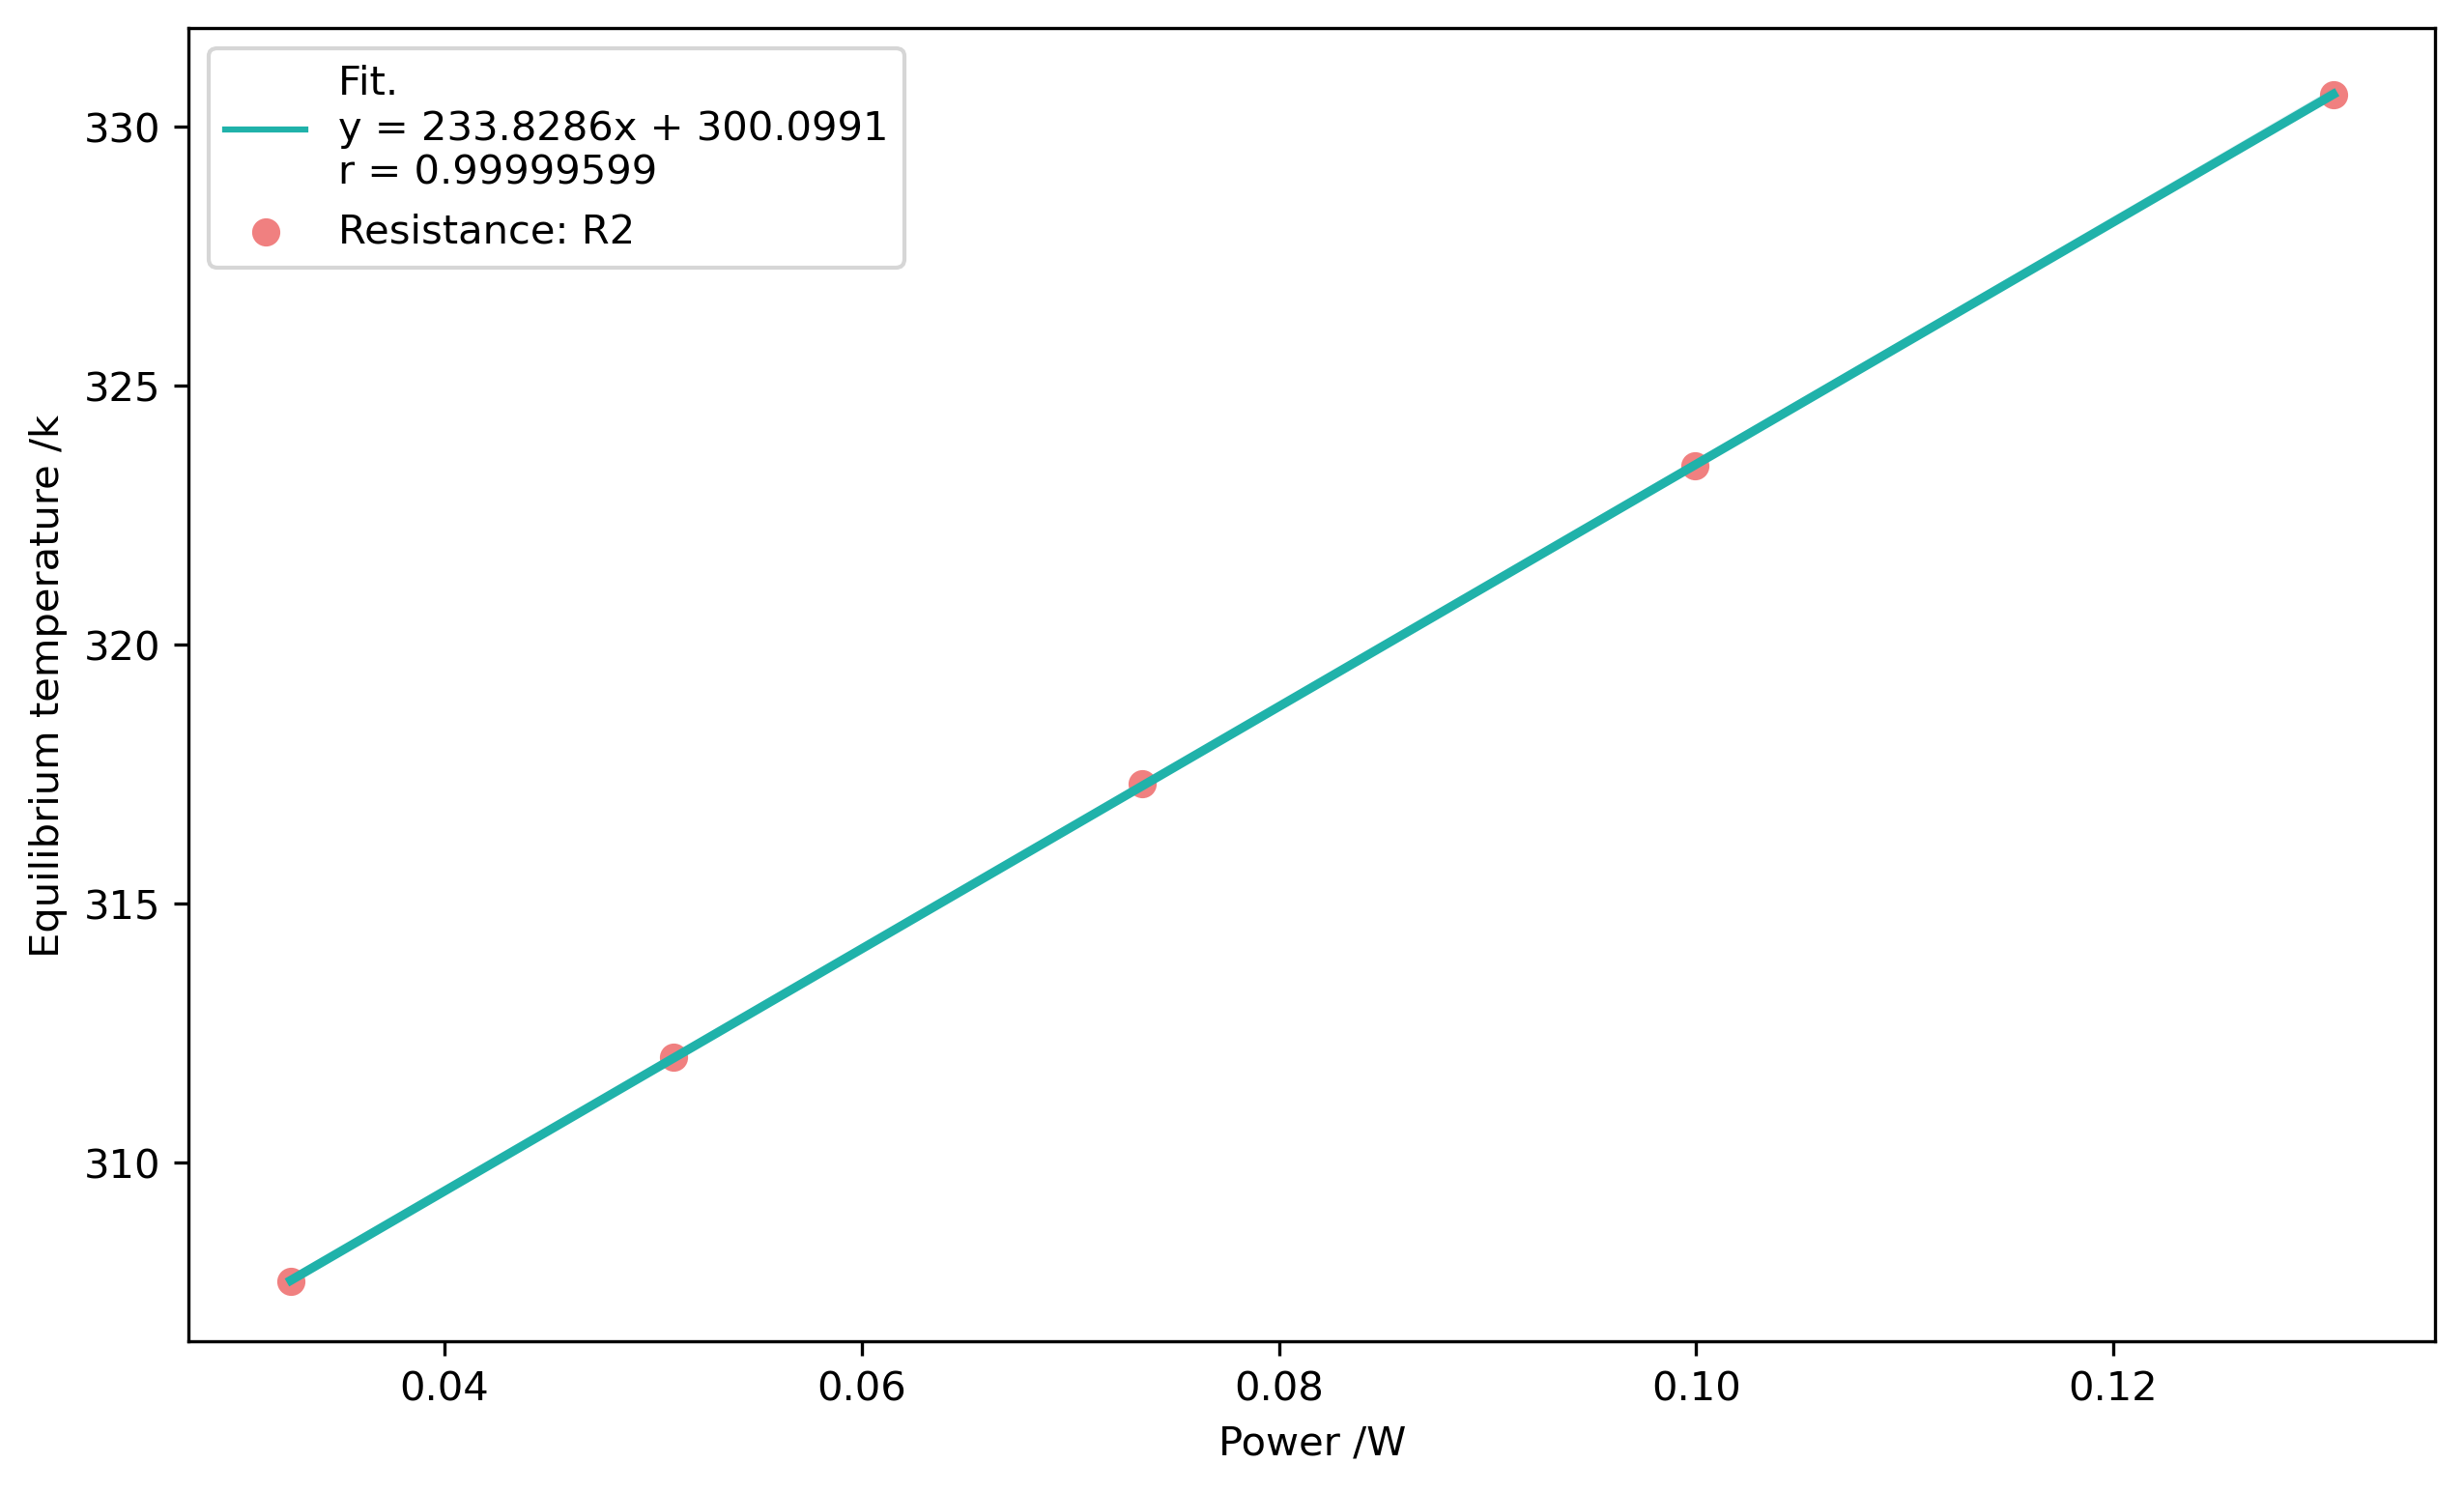
\includegraphics[width=0.3\textwidth]{attachments/fig.1.3.2.2.png}
		}

		\subfloat[$R_3 = 42.902 \Omega$]{\label{fig.1.3.2.3}
		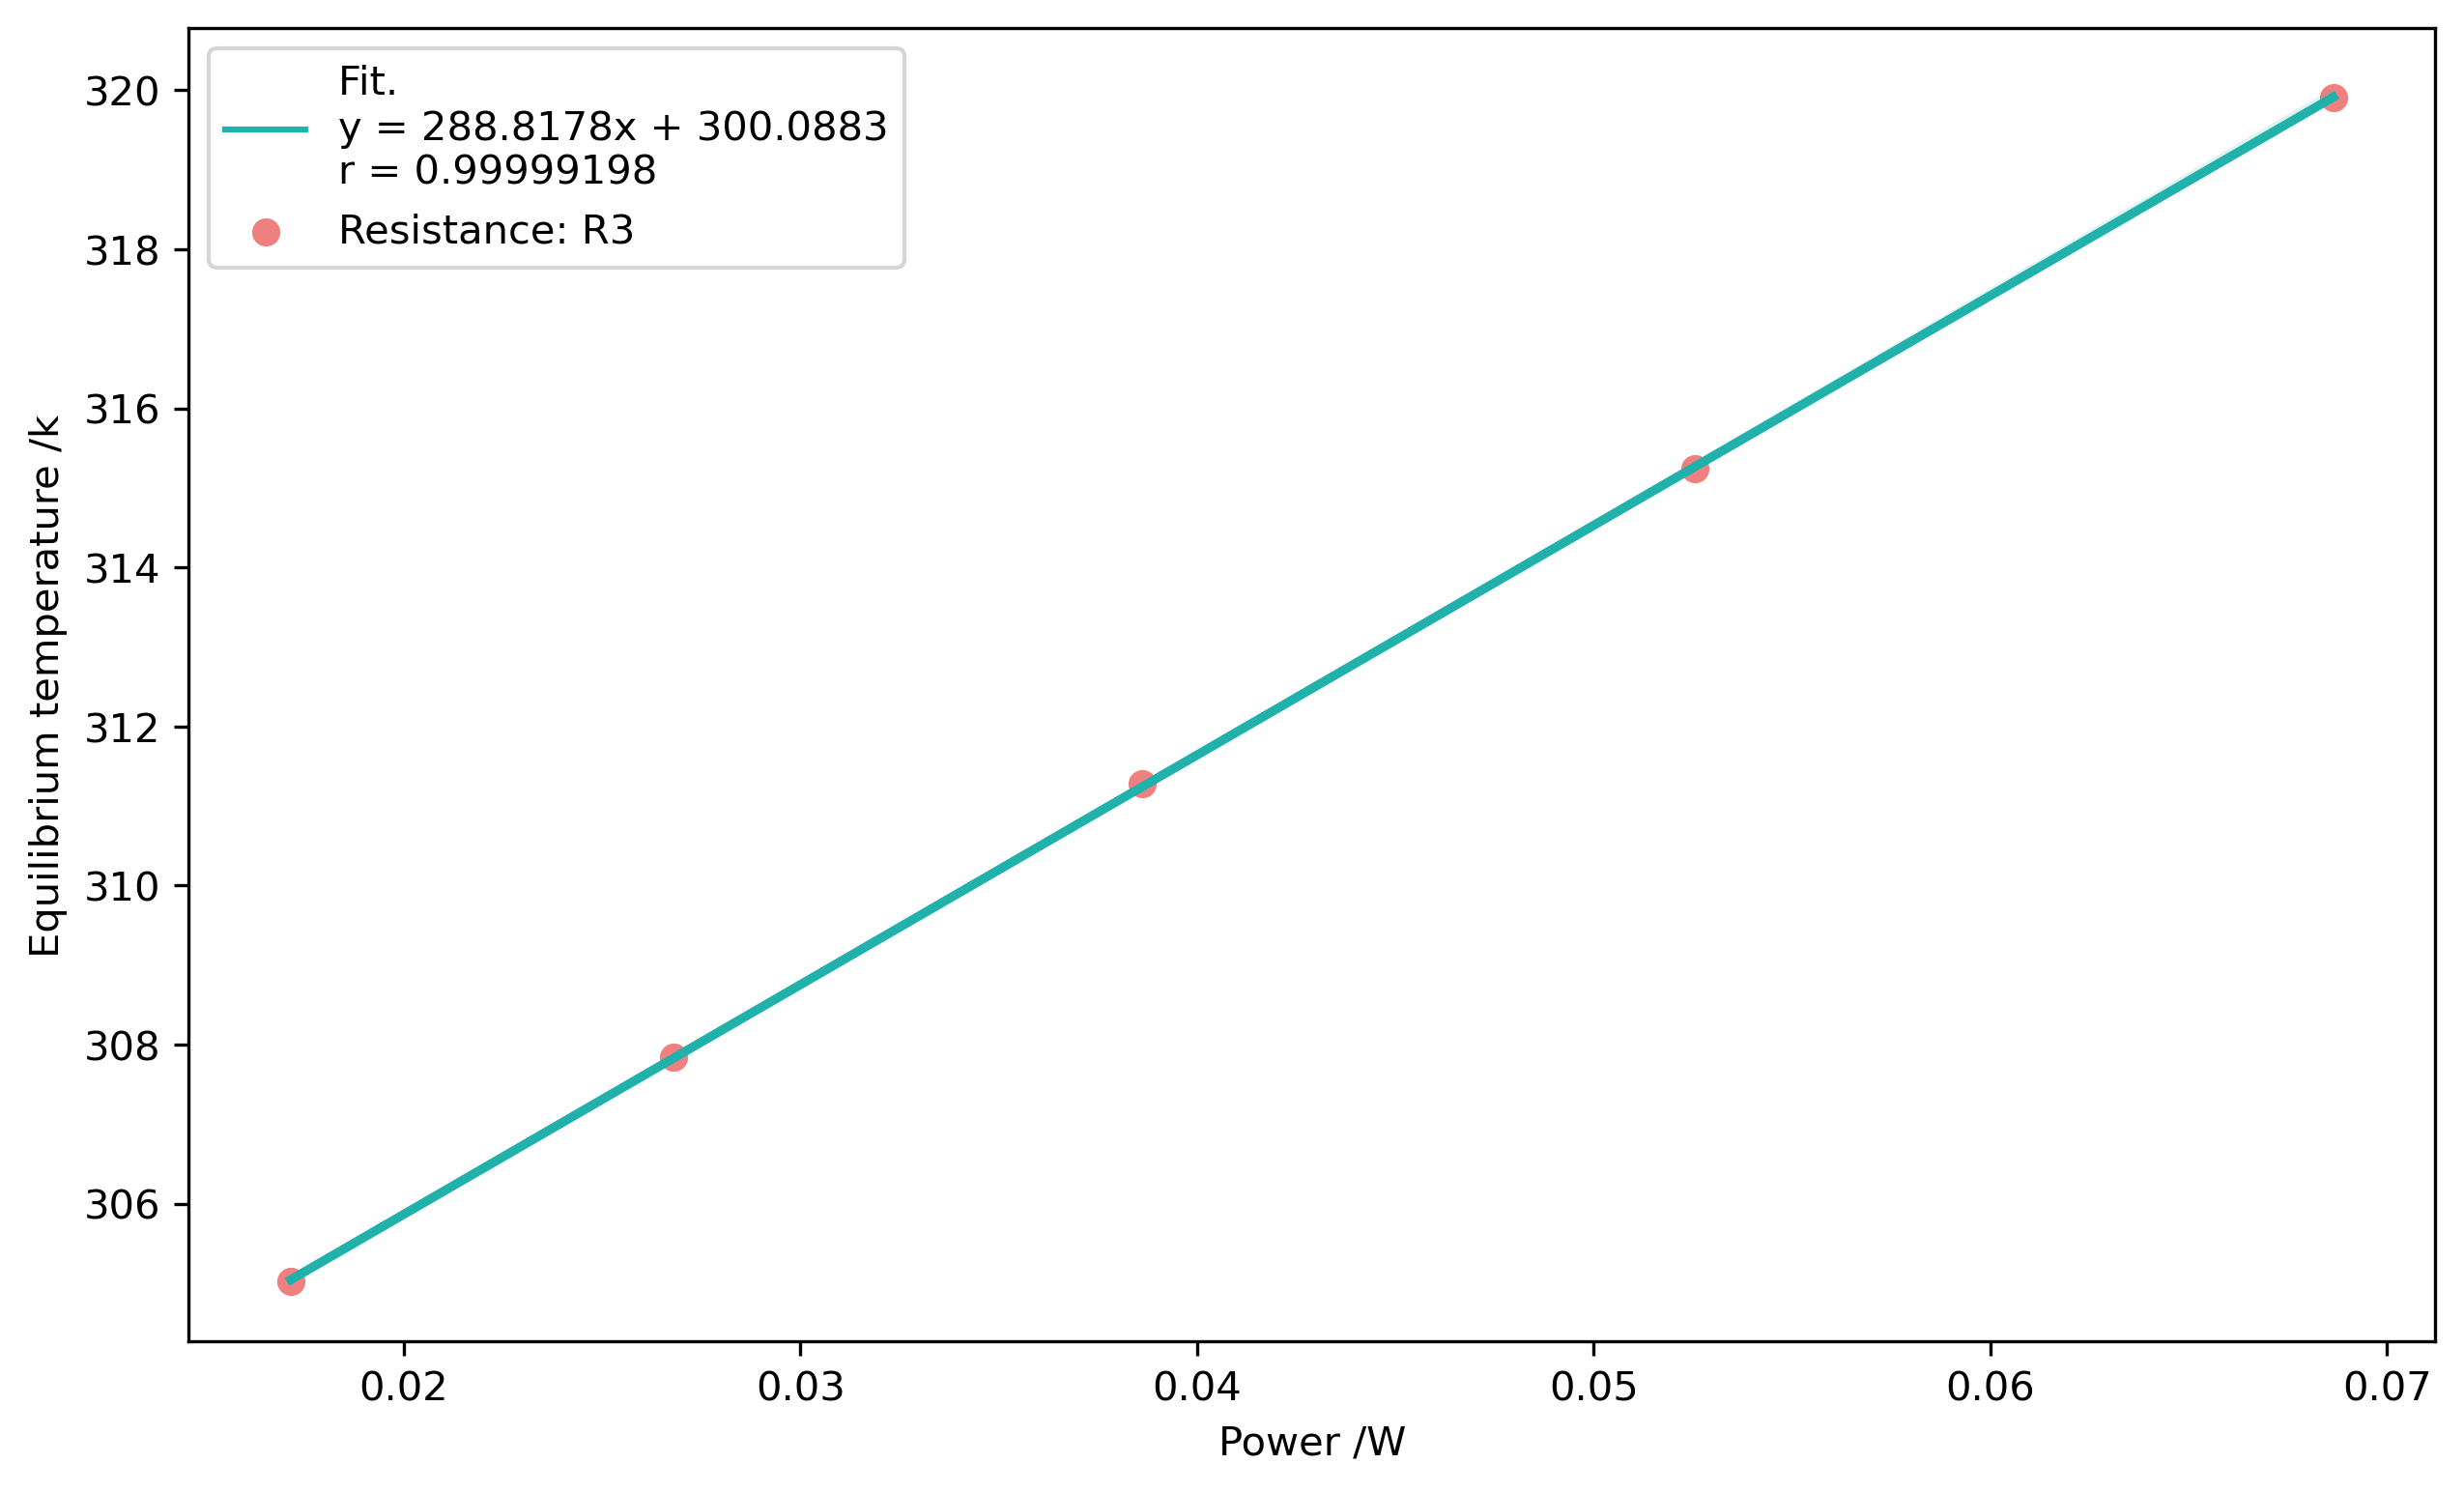
\includegraphics[width=0.3\textwidth]{attachments/fig.1.3.2.3.png}
		}
		\subfloat[$R_4 = 19.846 \Omega$]{\label{fig.1.3.2.4}
		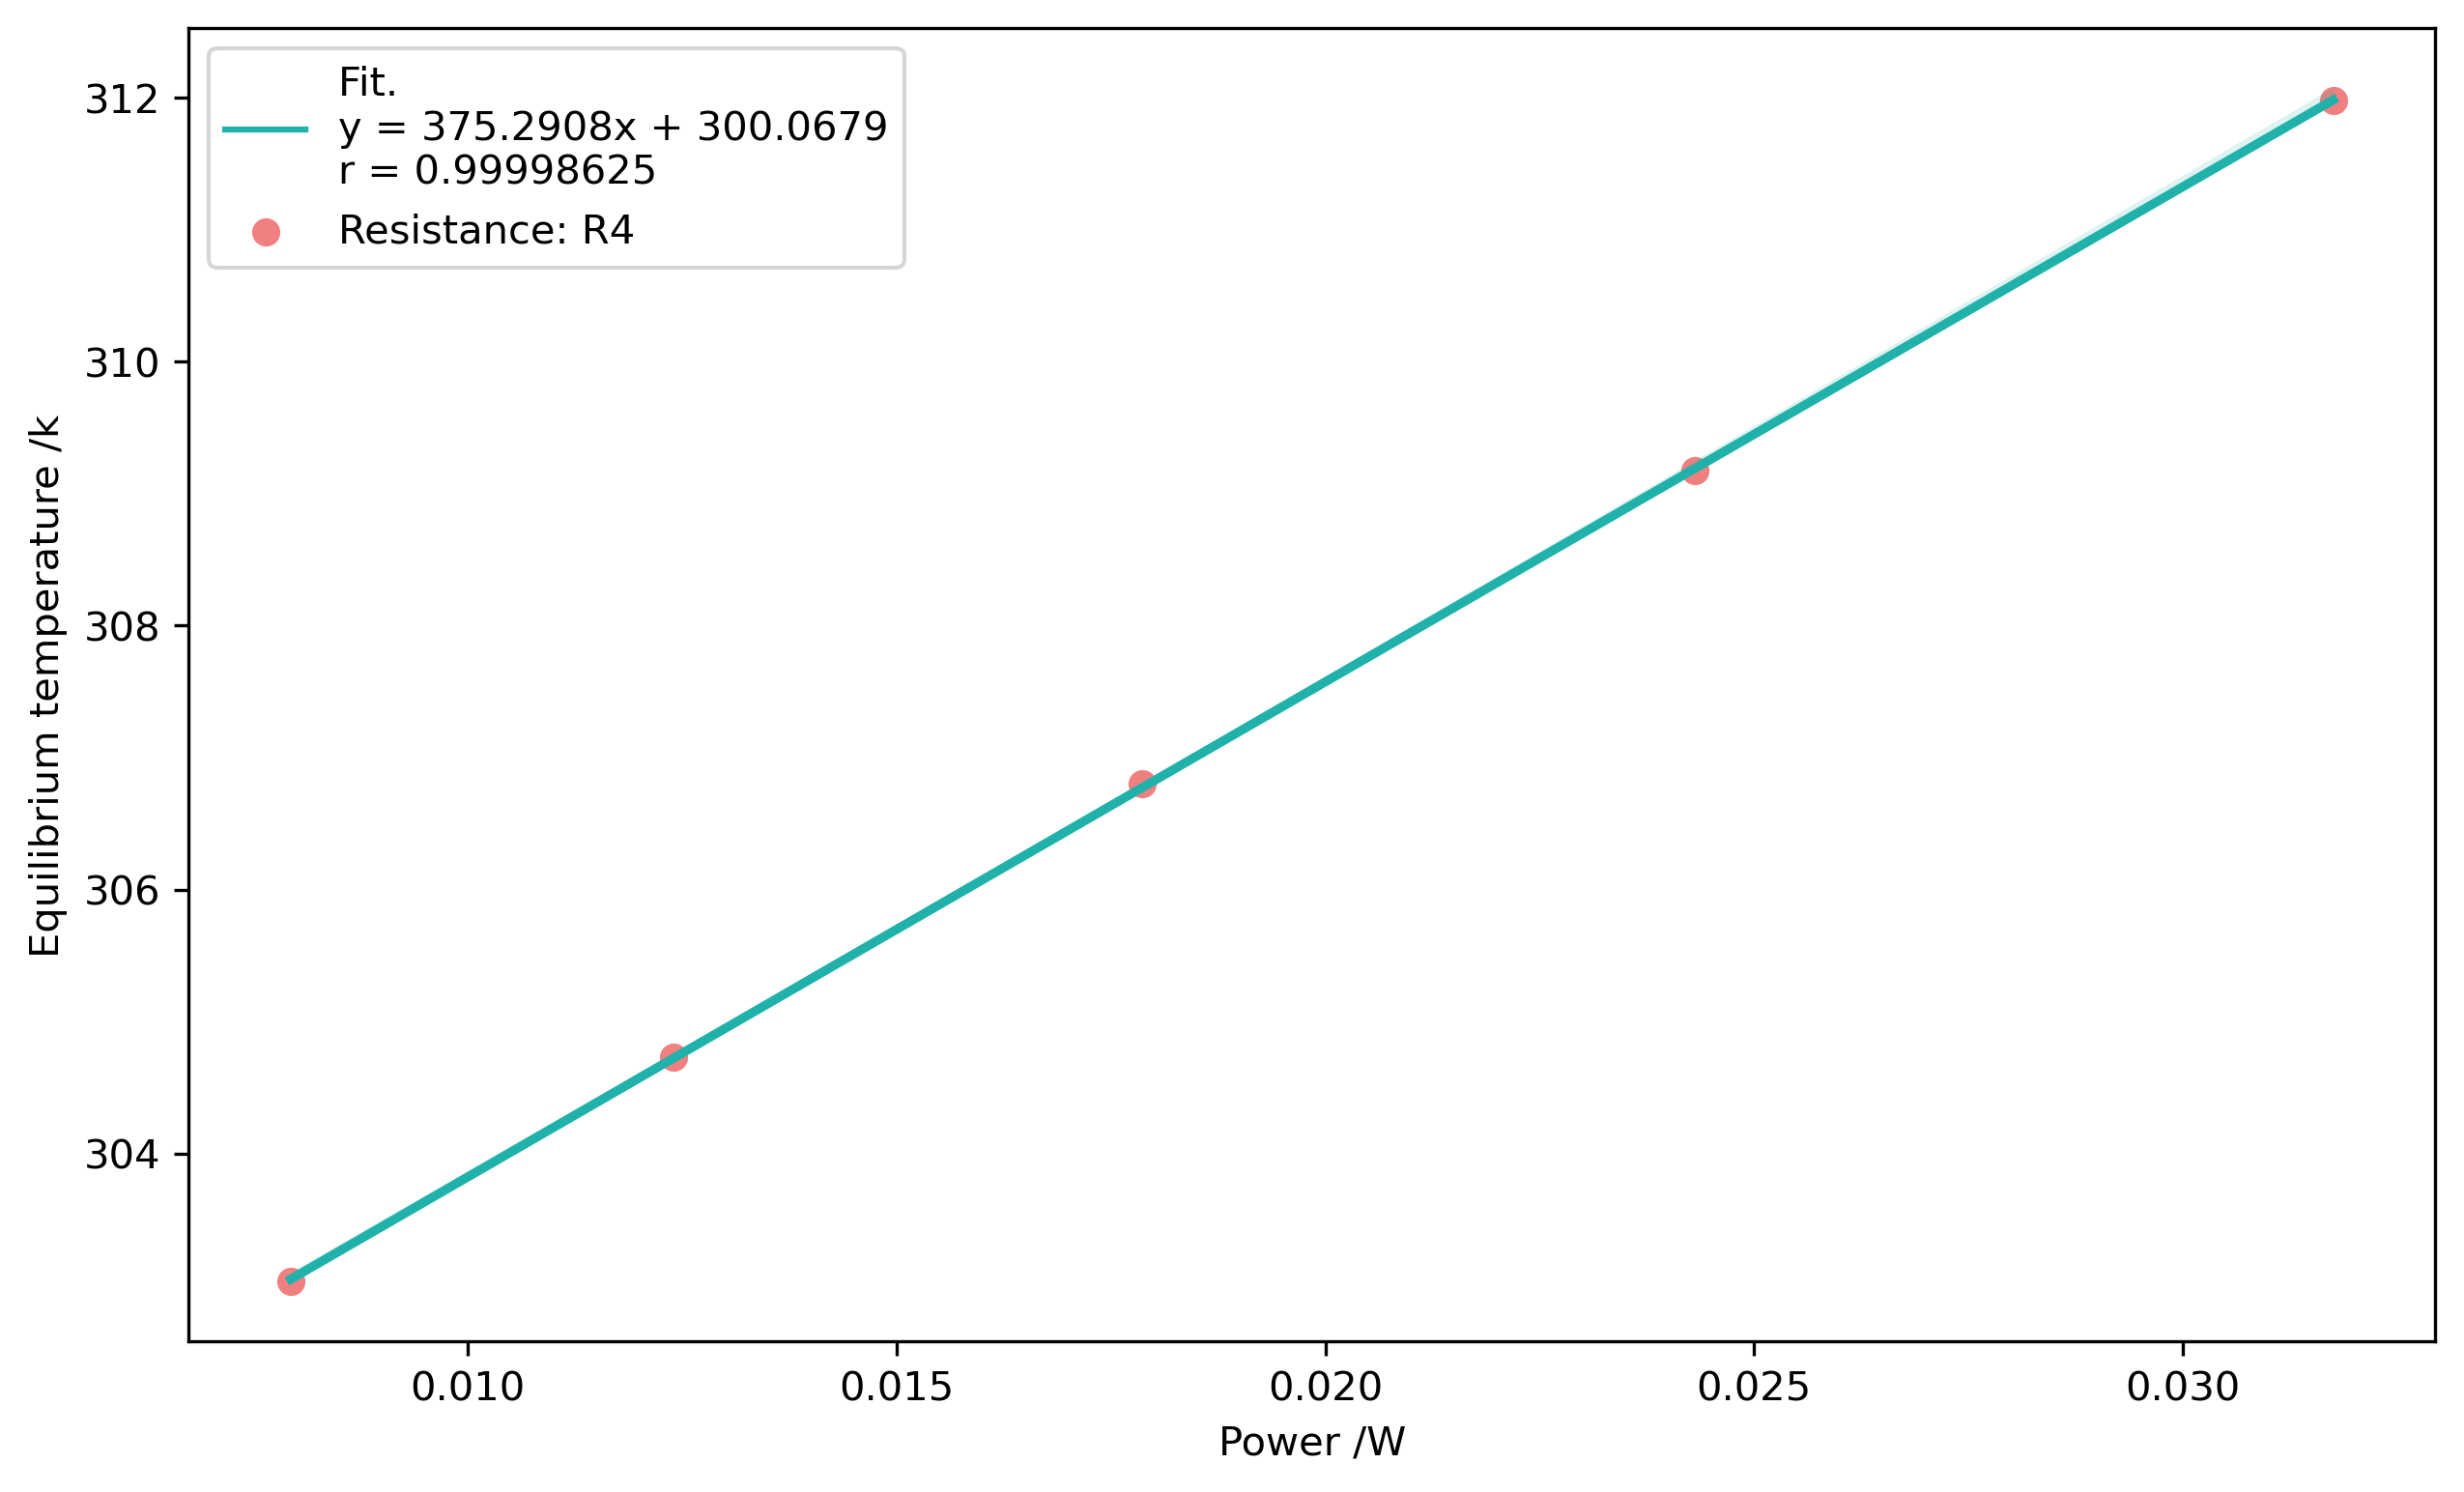
\includegraphics[width=0.3\textwidth]{attachments/fig.1.3.2.4.png}
		}
		\caption{\textbf{Correlation of equilibrium temperature and the heating power, simulation experiments of the complex model}}
		\label{fig.1.3.2}
	\end{figure*}


	\paragraph{C. Comparison of the three models}~
	\newline 
	\indent
	The equilibrium temperature of each reistor obtained from the real-world experiment, simulation on the ideal model and simulation on the complex model are summarized in Tab. \ref{tab.1}
	
	\begin{table*}[htbp]
	\centering
	\caption{\textbf{Summary of the equilibrium temperatures of the resistors}}
	\label{tab.1}
		\begin{tabular}{ccccc}
			\toprule
			Current & Resistor & Real-world Mod. & Sim. Ideal Mod. & Sim. Complex Mod. \\
			\midrule
			$0.020A$ & $R_1$ & 312.23 & 309.76 & 308.28 \\
			~ & $R_2$ & 308.63 & 307.49 & 307.71 \\
			~ & $R_3$ & 303.85 & 302.72 & 305.02 \\
			~ & $R_4$ & 301.41 & 300.87 & 303.03 \\
			$0.025A$ & $R_1$ & 318.17 & 315.72 & 312.92 \\
			~ & $R_2$ & 312.71 & 312.18 & 312.03 \\
			~ & $R_3$ & 305.67 & 304.73 & 307.84 \\
			~ & $R_4$ & 302.25 & 301.84 & 304.73 \\
			$0.030A$ & $R_1$ & 326.32 & 323.02 & 318.59 \\
			~ & $R_2$ & 318.60 & 317.92 & 317.31 \\
			~ & $R_3$ & 308.88 & 307.18 & 311.28 \\
			~ & $R_4$ & 304.25 & 303.02 & 306.80 \\
			$0.035A$ & $R_1$ & 335.46 & 331.86 & 325.20 \\
			~ & $R_1$ & 324.92 & 324.89 & 323.44 \\
			~ & $R_1$ & 311.73 & 310.20 & 315.25 \\
			~ & $R_1$ & 305.22 & 304.46 & 309.17 \\
			$0.040A$ & $R_1$ & 345.07 & 341.88 & 332.92 \\
			~ & $R_2$ & 332.22 & 332.77 & 330.62 \\
			~ & $R_3$ & 315.88 & 313.58 & 319.92 \\
			~ & $R_4$ & 307.81 & 306.09 & 311.98 \\
			\bottomrule
		\end{tabular}
	\end{table*}

	Out of our expectation, we found that the ideal model was even more accurate than the complex mode. 
	The heating time needed to reach the equilibrium and the final equilibrium temperature of the ideal model were all consistent with the real-world model, 
	while for the complex model, there's a great difference.
	We hypothesize that as the complex model involved much more details, the accuracy of the values of material properties and geometric dimensions becomes more essential and may have a more prevalent influence on the results.
	Due to lack of these necessary knowledge, the parameters were all set empirically, which may cause the results to be inaccurate.

	Anyway, the tendencies and general patterns of temperature changes are consistent among the three models, 
	which proves the effectiveness of these techniques in studying thermal conducting models with very complex boundary conditions.

	To further improve the performance of the model, accurate values of parameters involved in the model are required, and the geometric structure of the model is also required to improve.


		
		
	\subsection{The plate thermal model}
	\paragraph{A. Real-world experiment}~
	\newline 
	\indent
	As shown in Fig. \ref{fig.illus-2.2}, four samples of the same size were placed in a square grid with two heaters symmetrically embedded within two adjacent samples in both sides, which provides stable heat flux. 
	Outside the sample there were insulator which exchanged heat with surroundings following the Newton's cooling law.
	The two themocouples were placed at the central face and the heating face, respectively.

	The change of temperature of the central face (Fig. \ref{fig.2.1.1}) and the temperature difference between the heating face and the central face (Fig. \ref{fig.2.1.2}) were obtained for samples made of rubber or organic glass.
	Results show that the for both materials, after a short period of non-linear increasing of the temperature, the system finally reached the quasi-stable state, in which the temperature was directly proportional to the heating time.
	At the same time, the temperature difference between the heating face and the central face also became stable.

	The equilibrium temperature difference and the changing rate of the central-face temperature were calculated, which are summarized in the Tab. \ref{tab.2}. 

	Simultaneously, the simulation experiments were conducted.
	\begin{figure*}[htbp]
		\centering
		\subfloat[Temperature of the central face]{\label{fig.2.1.1}
		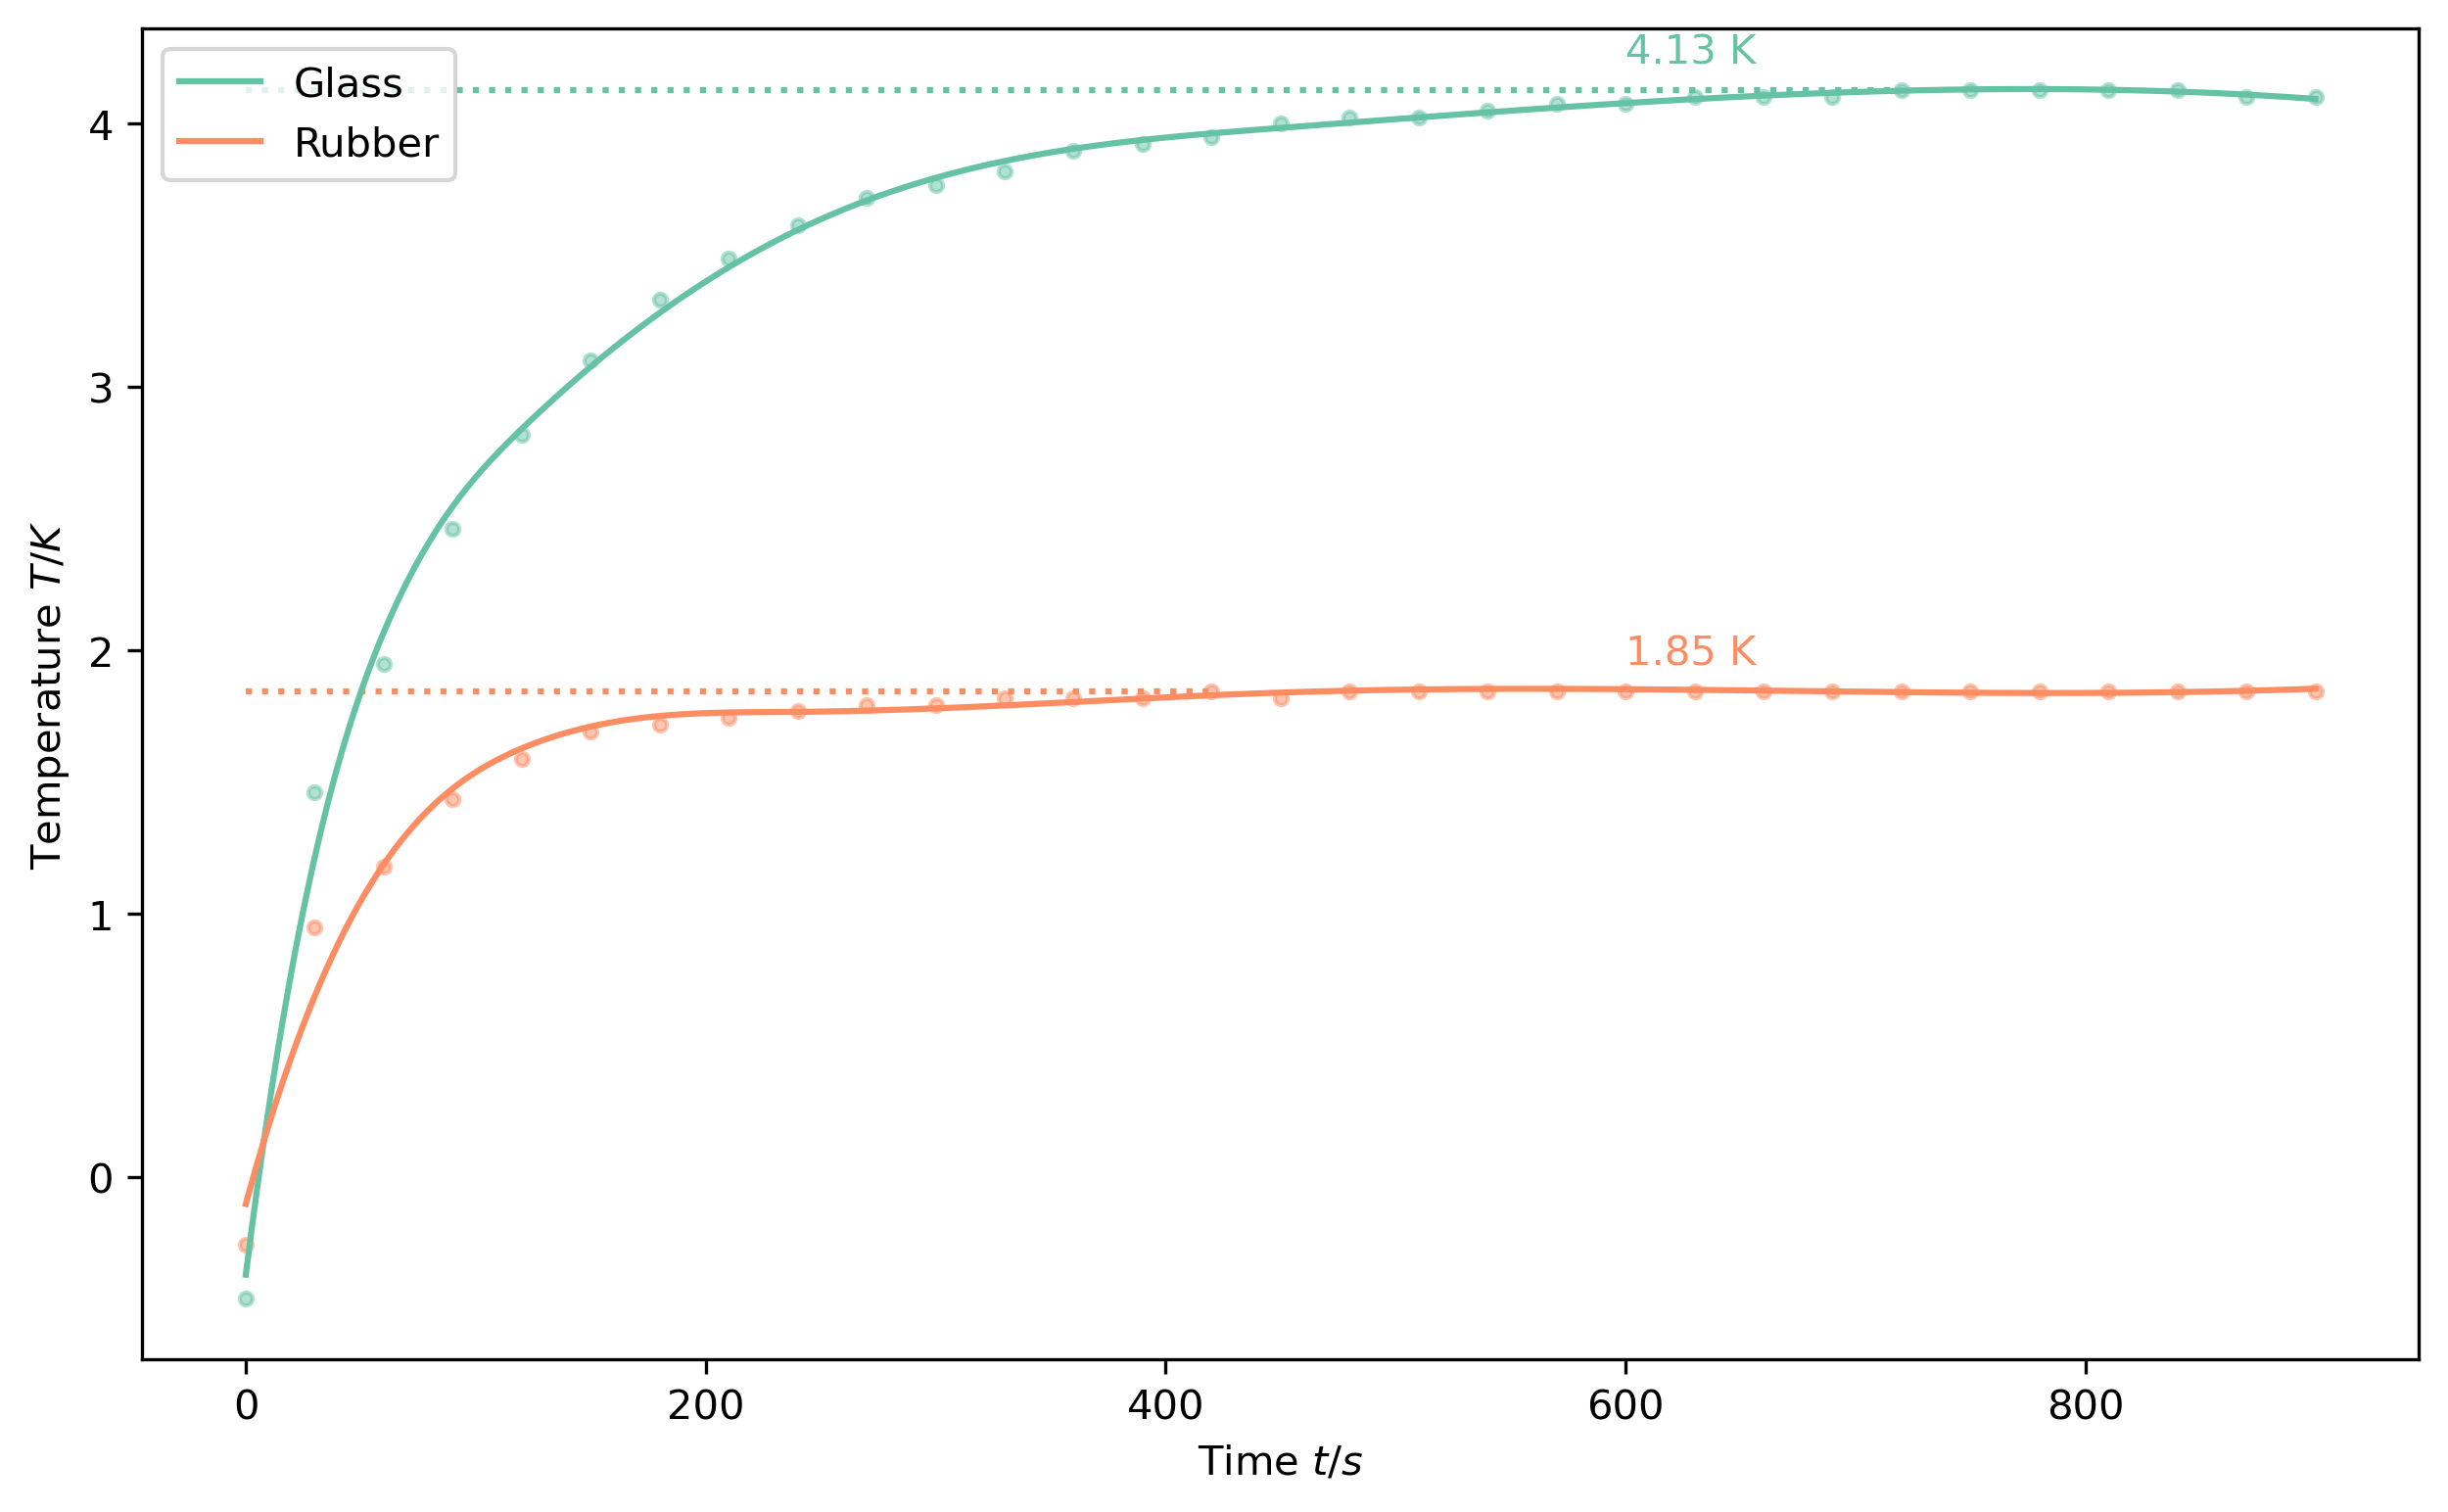
\includegraphics[width=0.4\textwidth]{attachments/fig.2.1.1.png}
		}		
		\subfloat[Temperature difference]{\label{fig.2.1.2}
		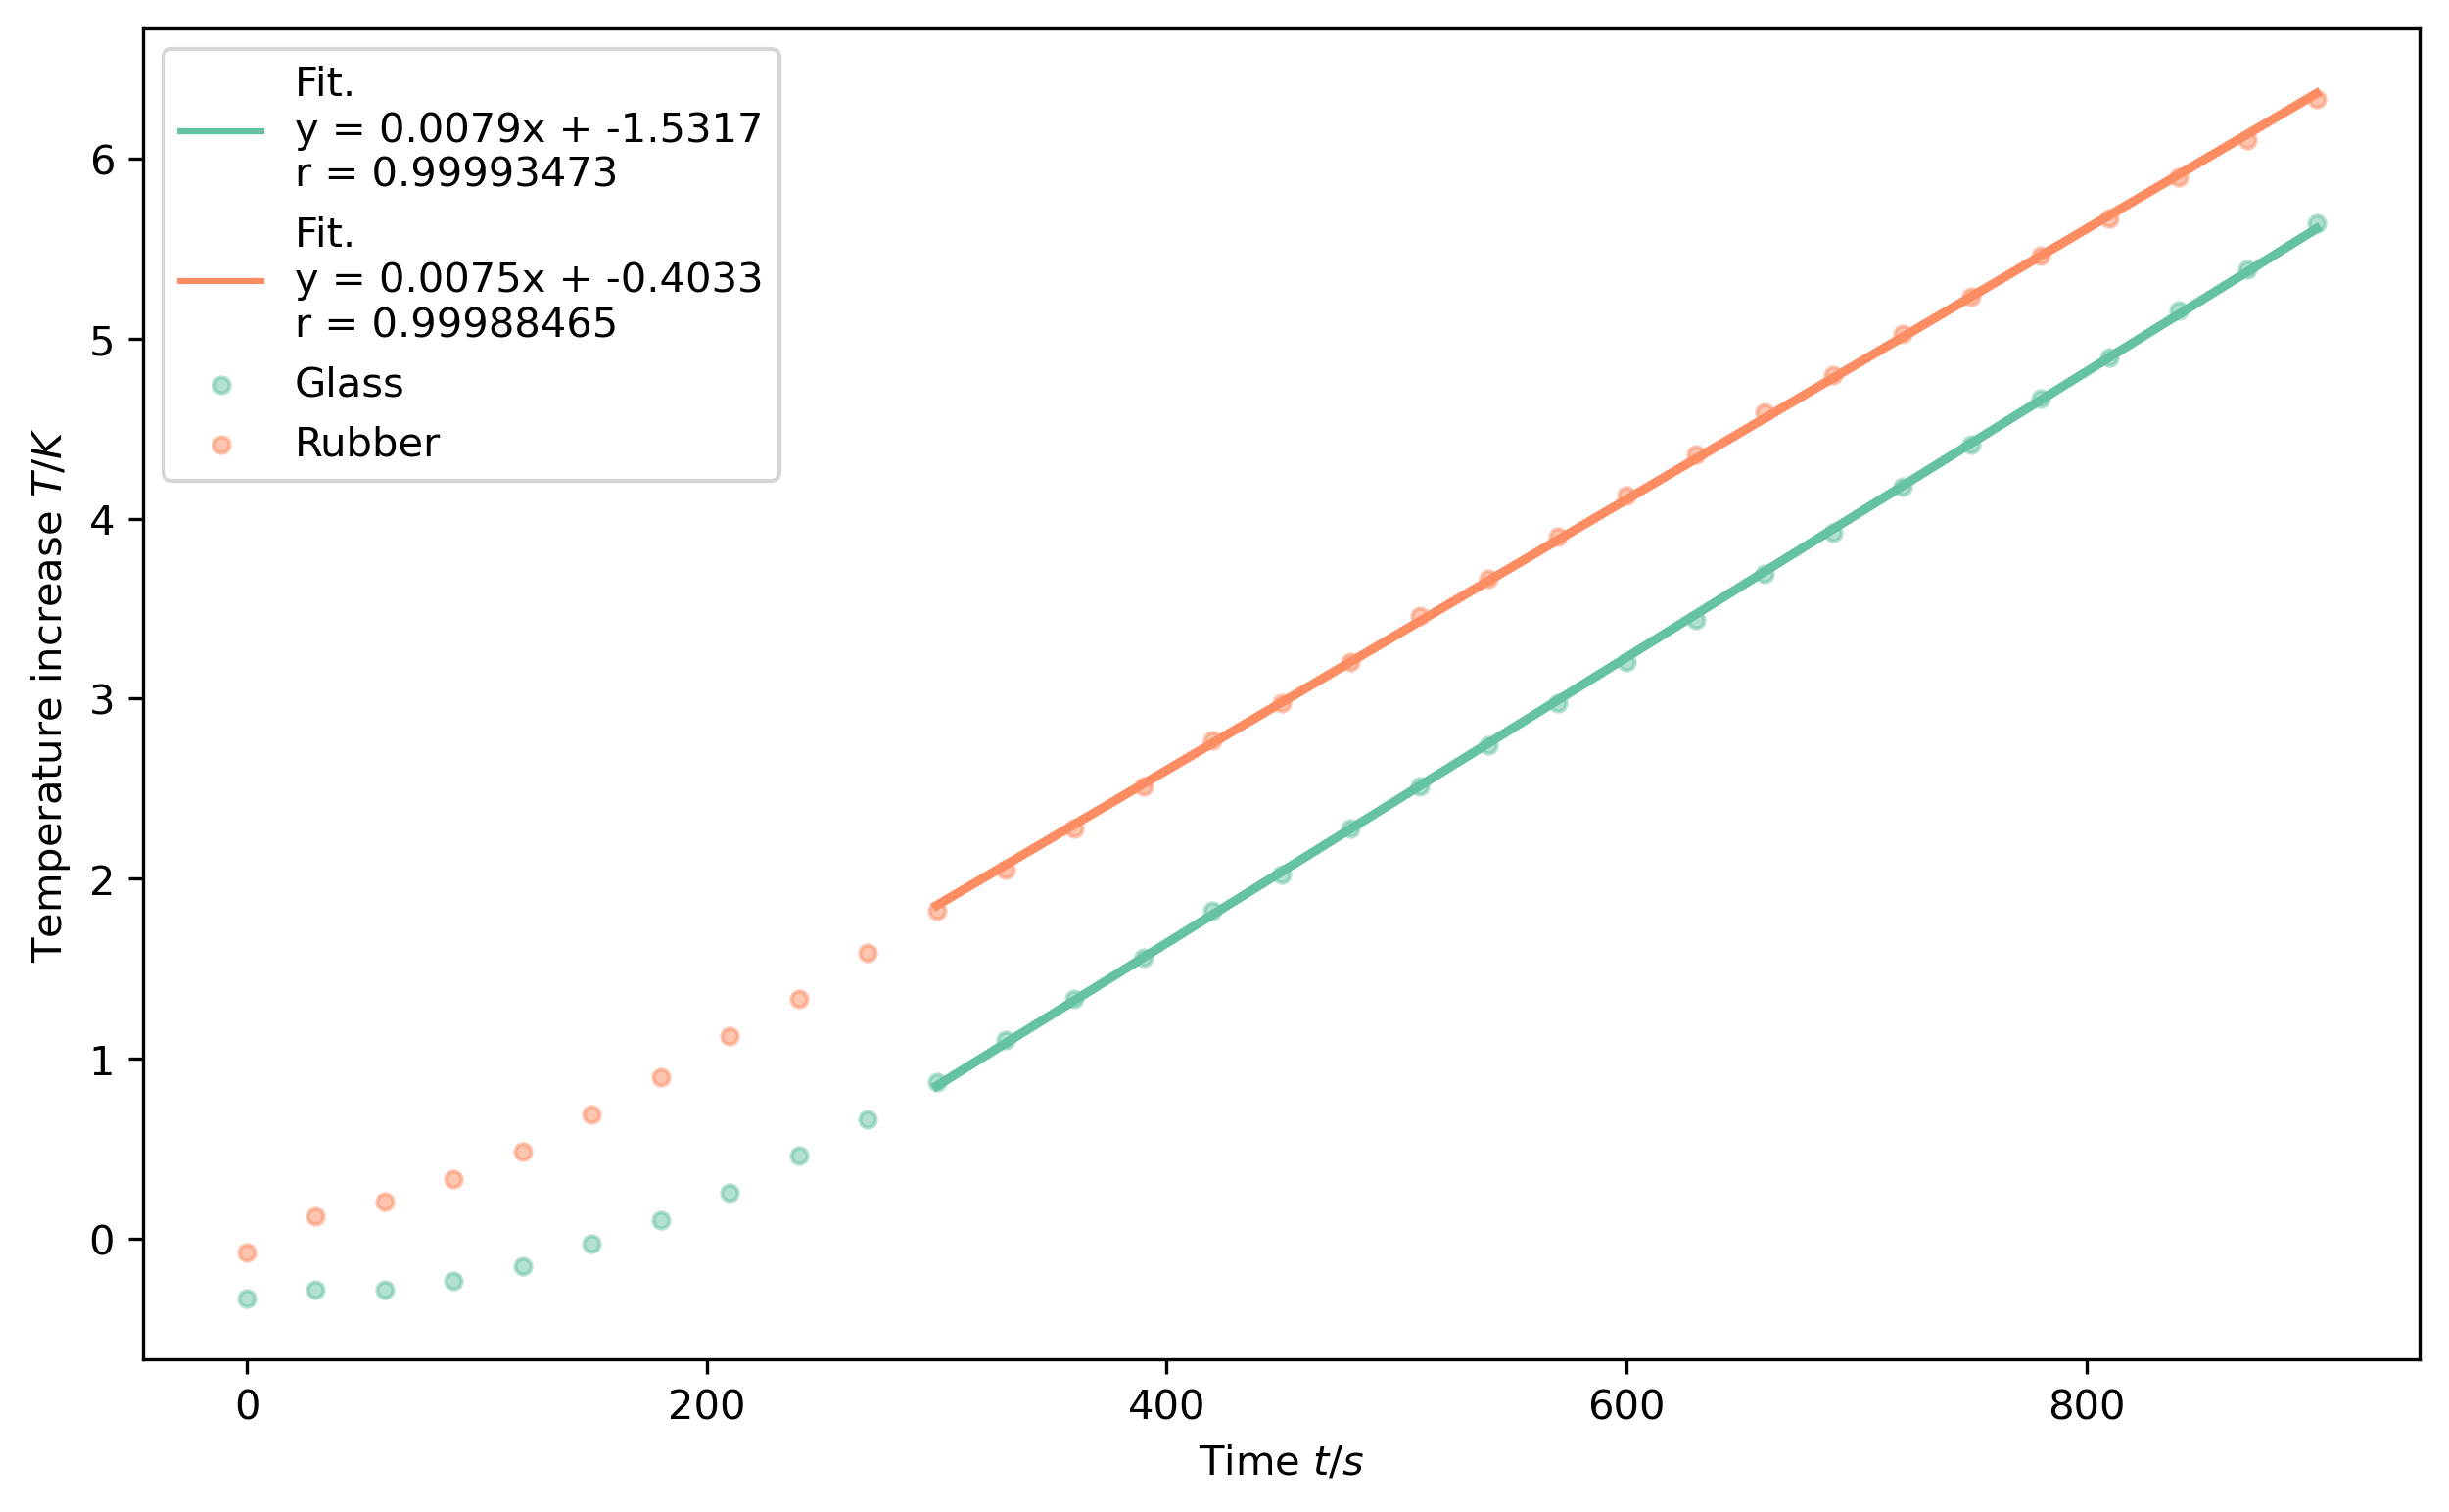
\includegraphics[width=0.4\textwidth]{attachments/fig.2.1.2.png}
		}
		\caption{\textbf{Thermal conduction of rubber or glass, real-world experiments}}
		\label{fig.2.1}
	\end{figure*}


	\paragraph{B1. Simulation: The ideal model}~
	\newline 
	\indent
	To begin with, we first built the ideal thermal model (As illustrated in Fig. \ref{fig.illus-1.2}) and run the simulation on COMSOL platform.
	The geometric model of the ideal resistor thermal model is shown in Fig. \ref{fig.2.2.0}. 
	The surfaces of the model were allowed to exchange heat with surroundings following the Newton's cooling law.
	With stable current provided, the two membrane-like heaters continuously provided stable heat flux, and the temperature of the samples began to raise. 
	The change of temperature of the central face (Fig. \ref{fig.2.2.1}) and the temperature difference between the heating face and the central face (Fig. \ref{fig.2.2.2}) were obtained for samples made of rubber or organic glass.

	Results show that at the quasi-stable state, the temperature was directly proportional to the heating time and the temperature difference between the heating face and the central face was stable, which is consistent with the real-world experiment.

	\begin{figure*}[htbp]
		\centering
		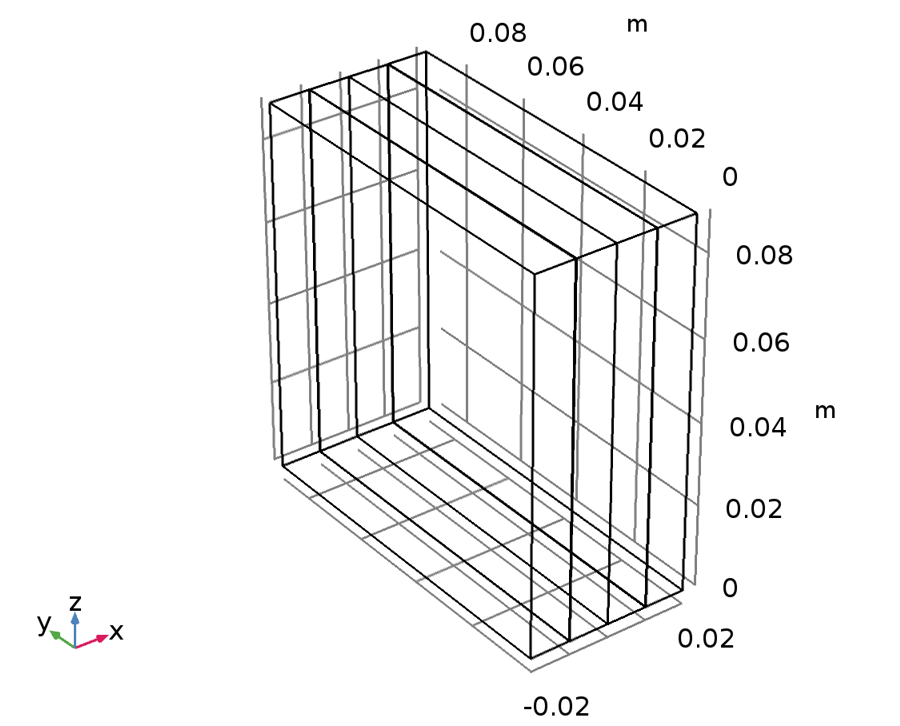
\includegraphics[width=0.4\textwidth]{attachments/fig.2.2.0.png}
		\caption{\textbf{The geometric model of the ideal plate model}}
		\label{fig.2.2.0}
	\end{figure*}

	\begin{figure*}[htbp]
		\centering
		\subfloat[Temperature of the central face]{\label{fig.2.2.1}
		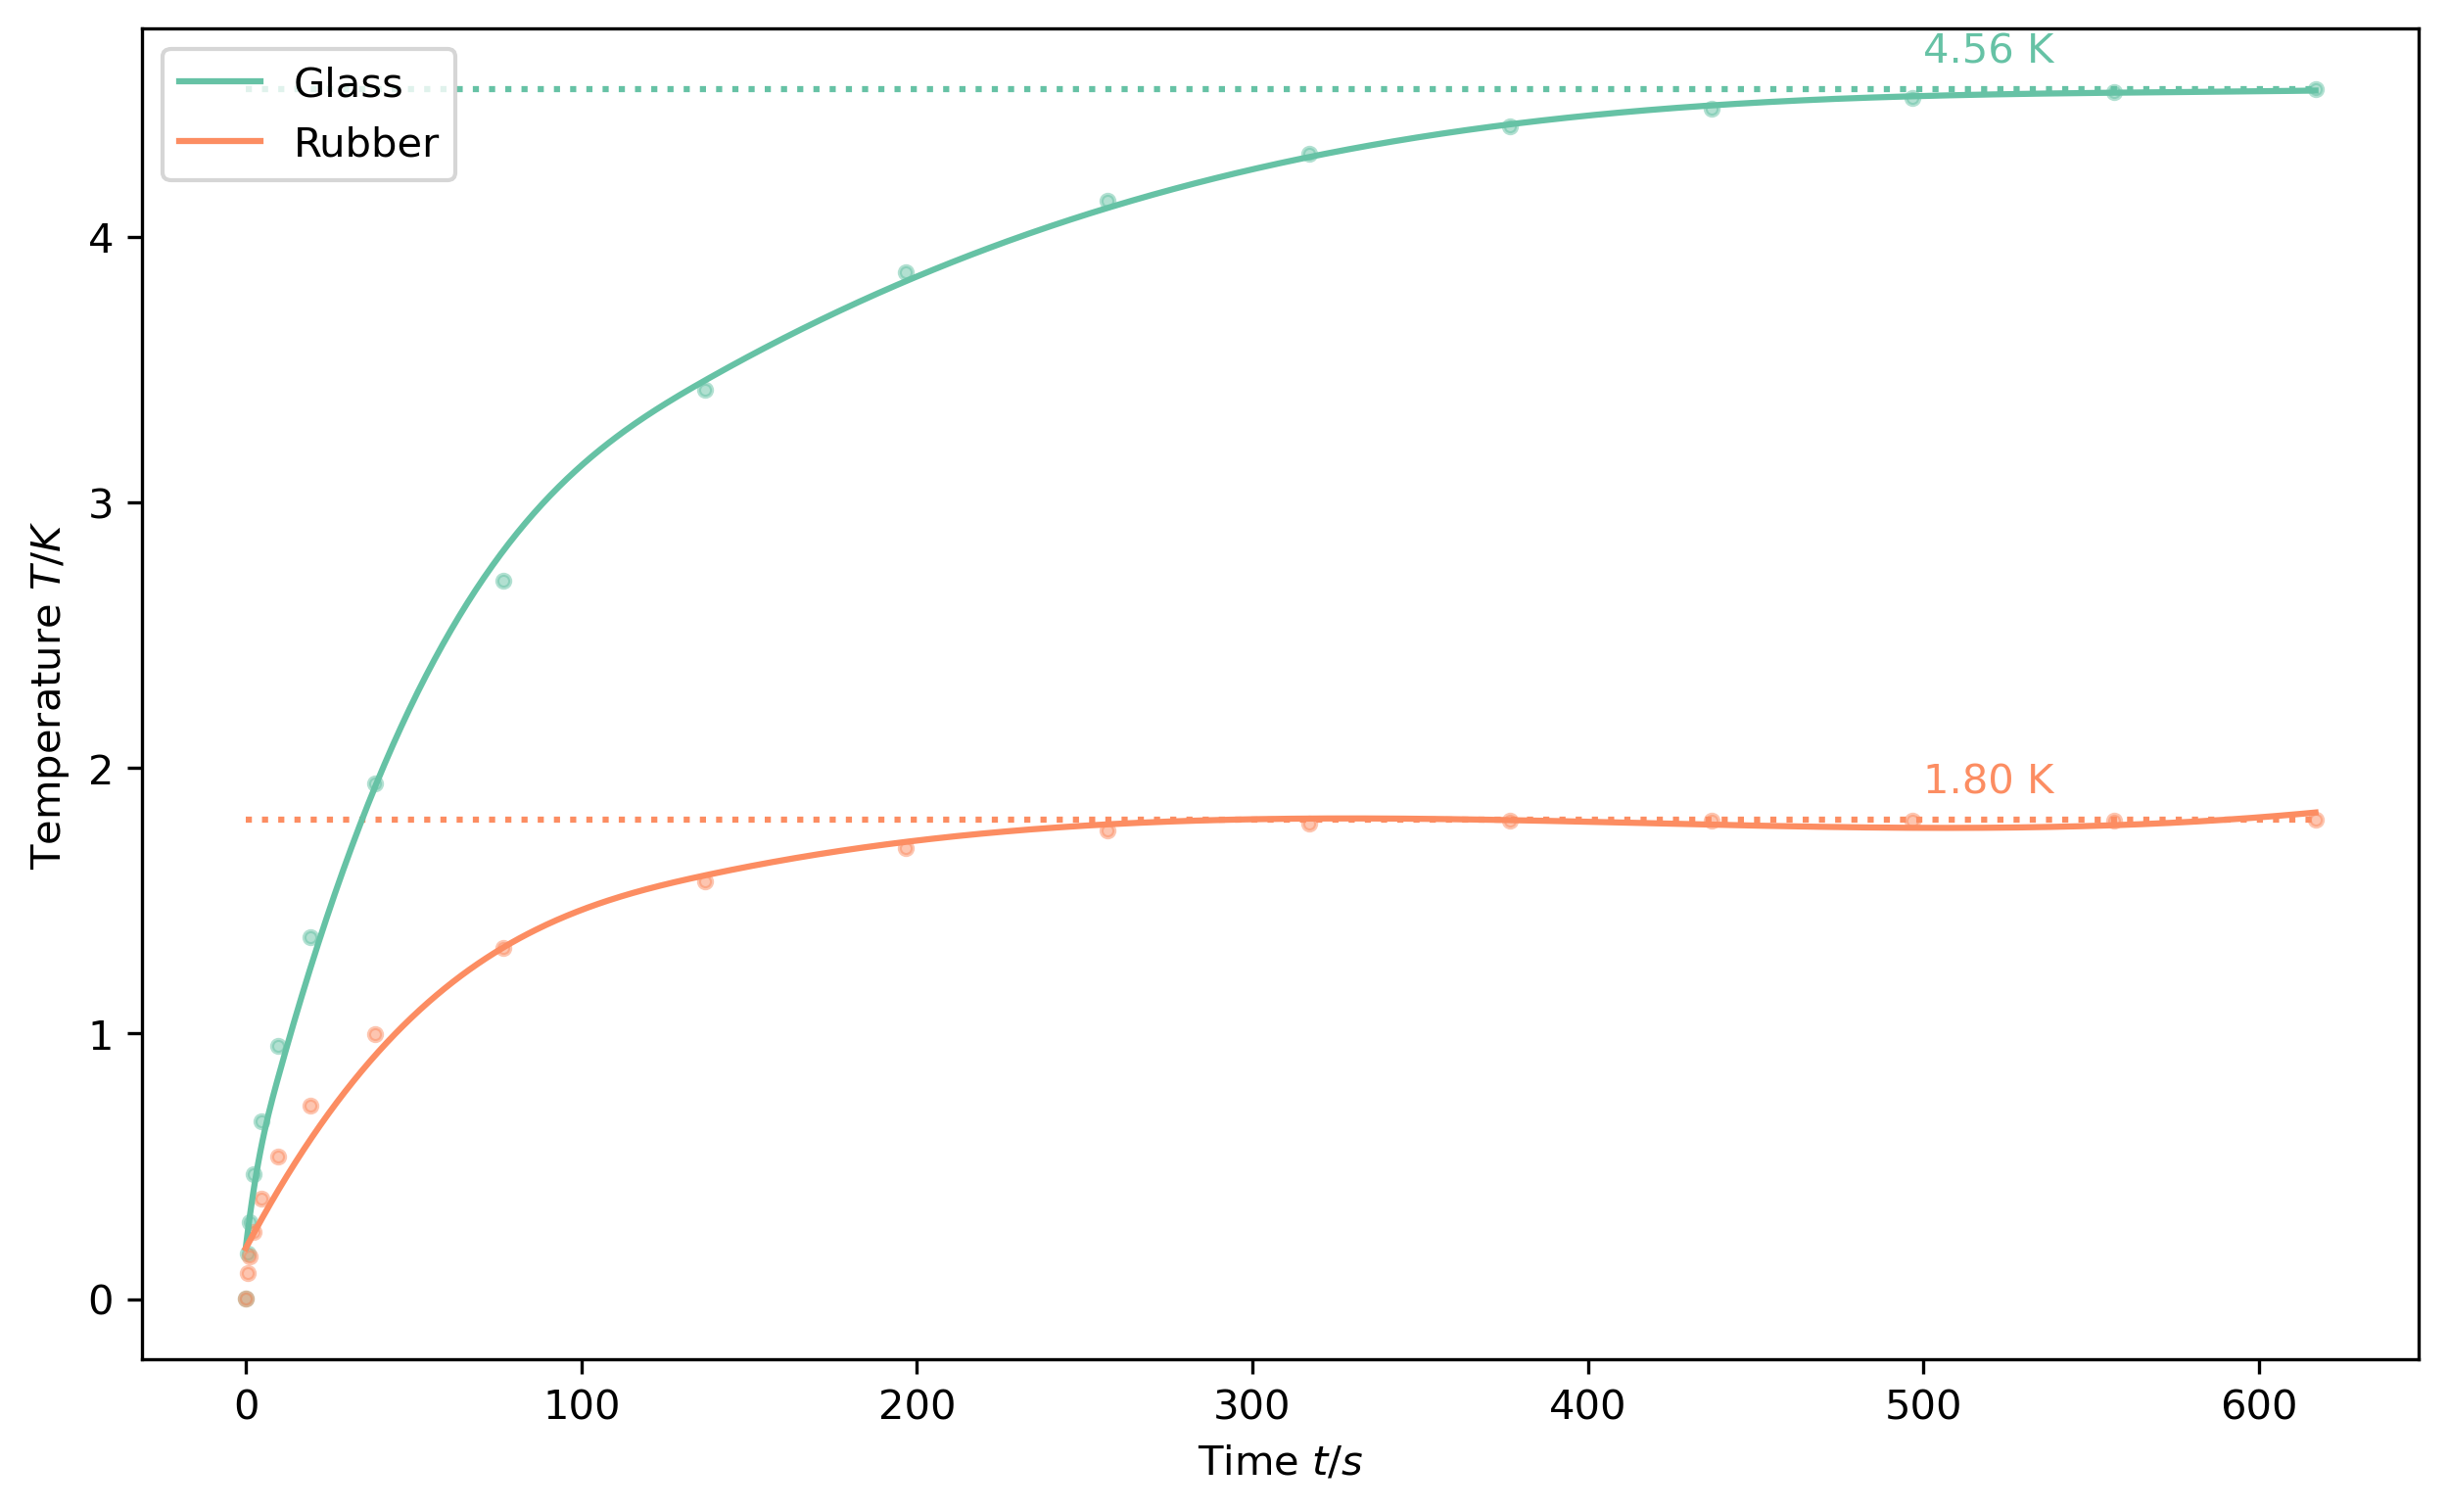
\includegraphics[width=0.4\textwidth]{attachments/fig.2.2.1.png}
		}		
		\subfloat[Temperature difference]{\label{fig.2.2.2}
		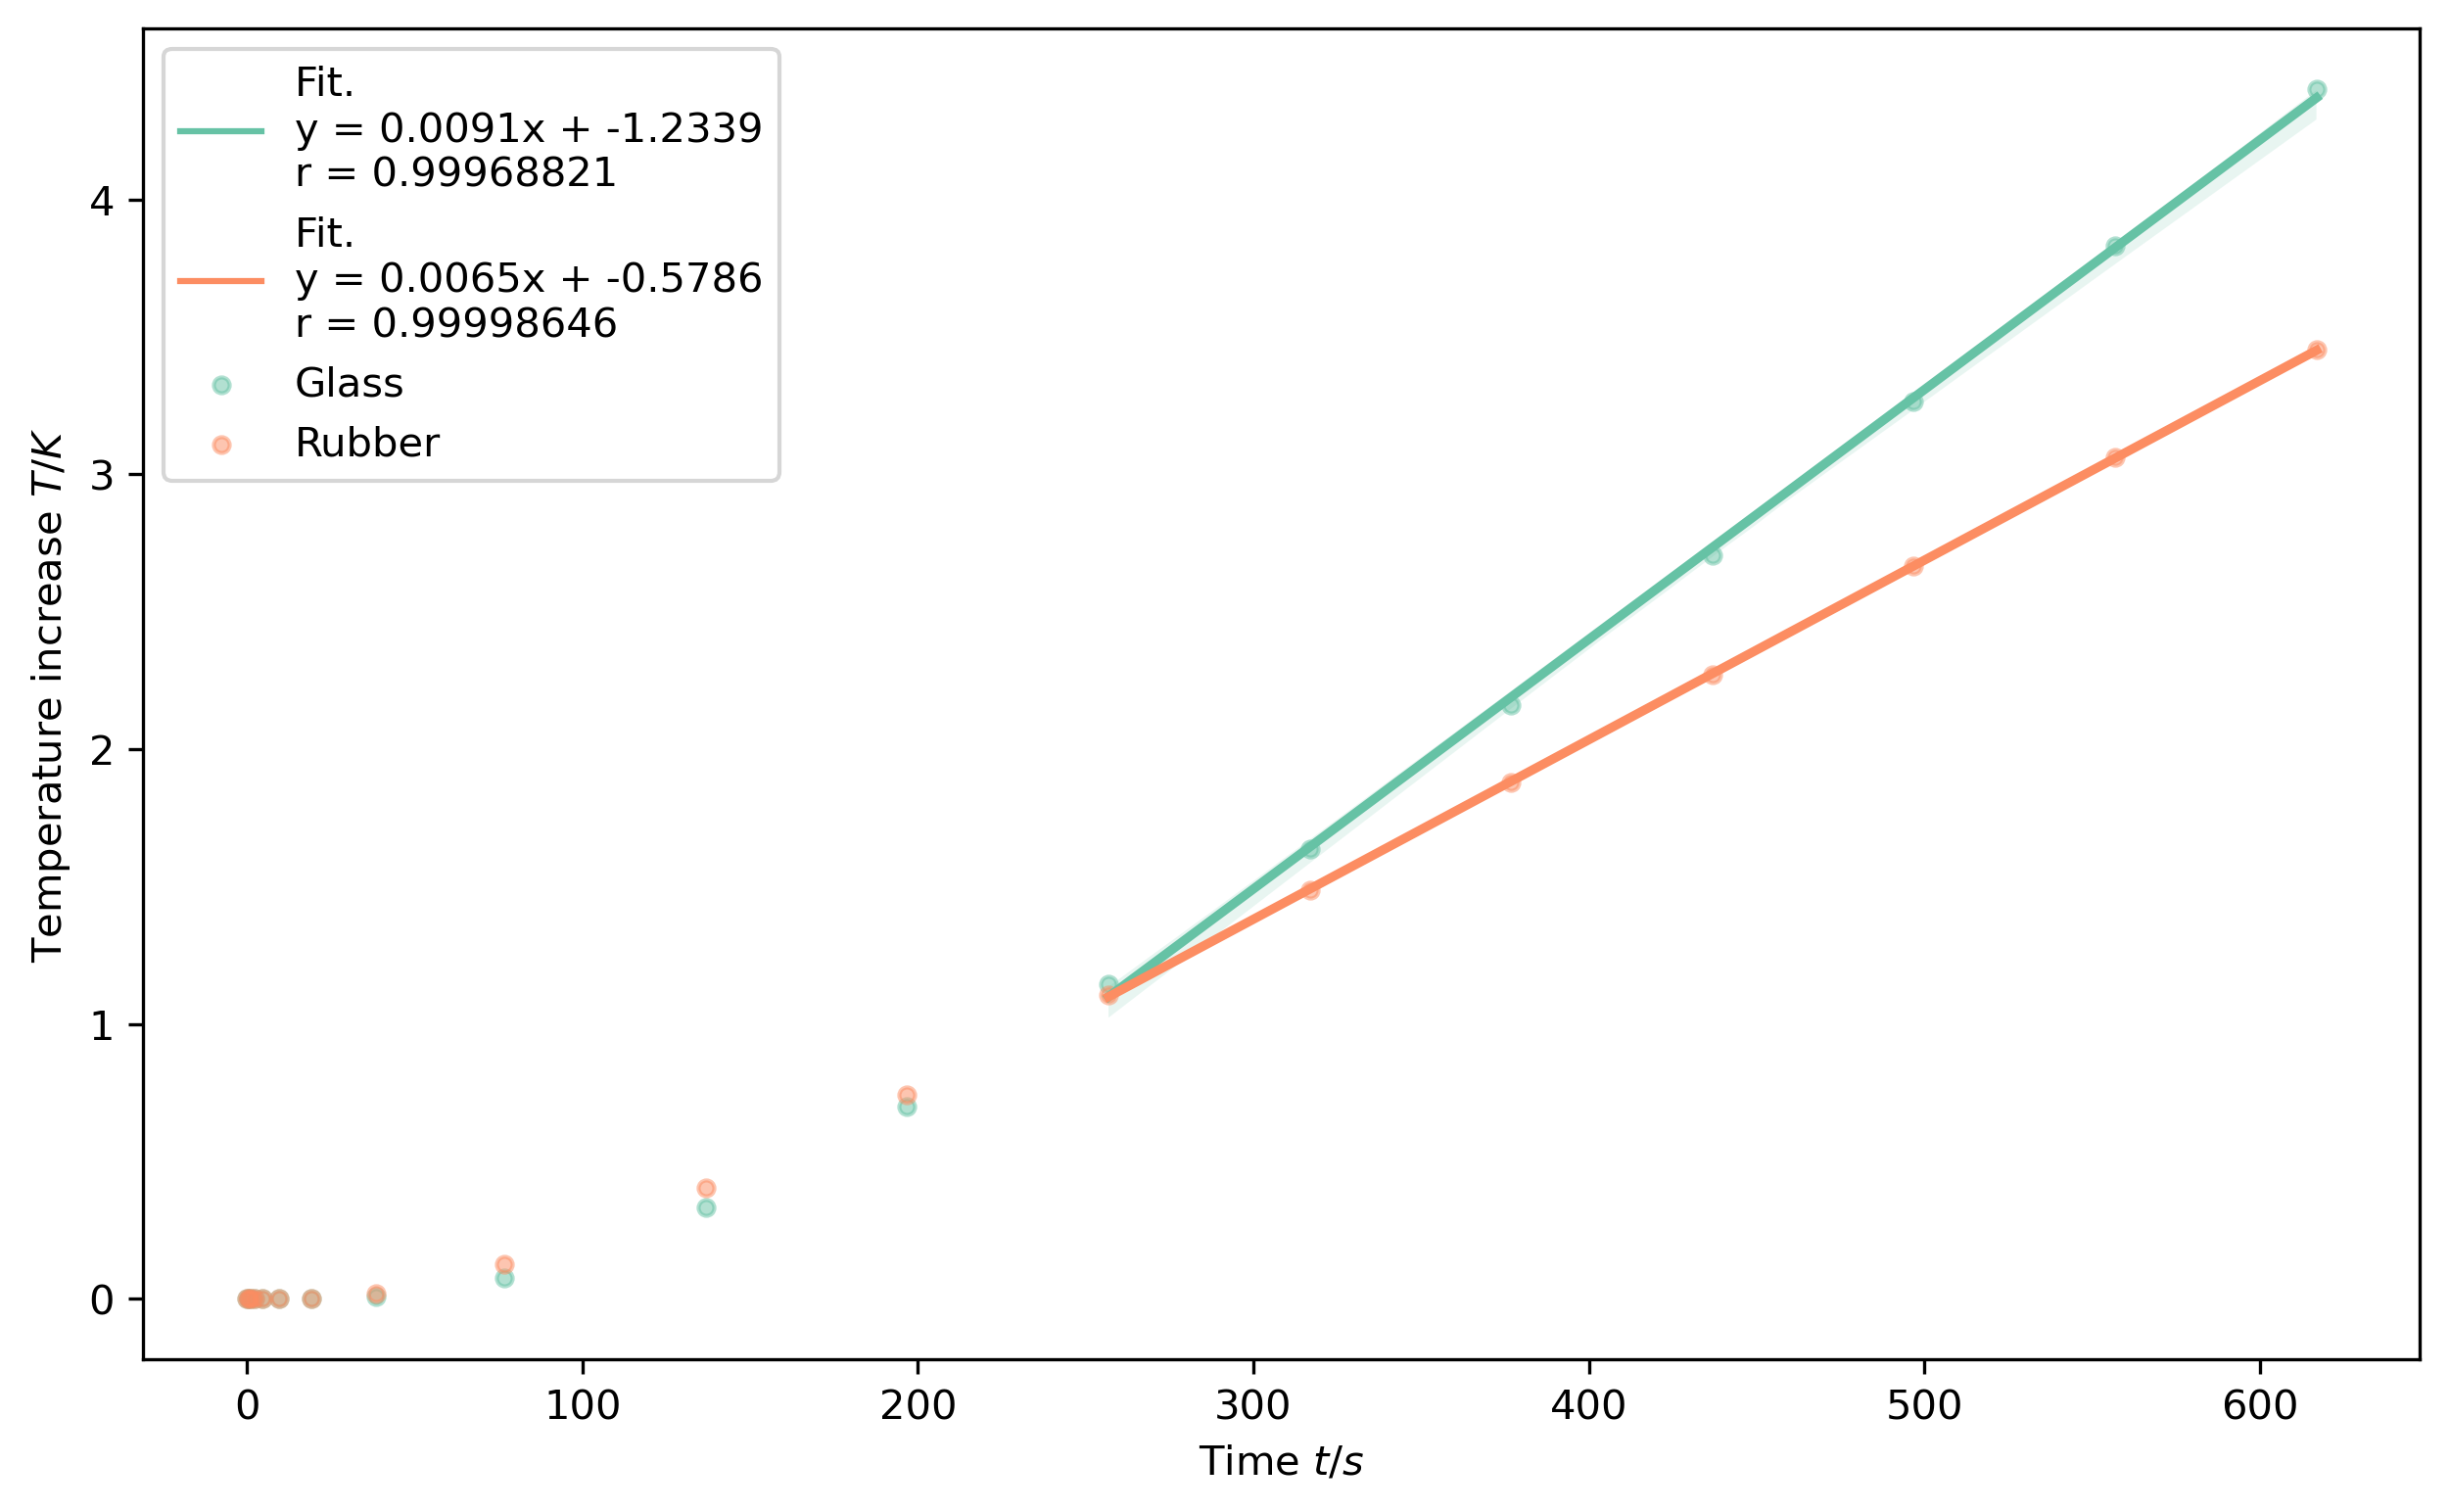
\includegraphics[width=0.4\textwidth]{attachments/fig.2.2.2.png}
		}
		\caption{\textbf{Thermal conduction of rubber or glass, simulation experiments of the ideal model}}
		\label{fig.2.2}
	\end{figure*}


	\paragraph{B2. Simulation: The complex model}~
	\newline 
	\indent
	Next, we built the complex plate thermal model in which the samples were embedded in the insulator and run the simulation on the COMSOL platform.
	The geometrical model of the complex thermal model is shown in Fig. \ref{fig.2.3.0}.
	With stable current provided, the two membrane-like heaters continuously provided stable heat flux, and the temperature of the samples began to raise. 
	The change of temperature of the central face (Fig. \ref{fig.2.3.1}) and the temperature difference between the heating face and the central face (Fig. \ref{fig.2.3.2}) were obtained for samples made of rubber or organic glass.

	Results show that at the quasi-stable state, the temperature was directly proportional to the heating time and the temperature difference between the heating face and the central face was stable, which is consistent with the real-world experiment.

	\begin{figure*}[htbp]
		\centering
		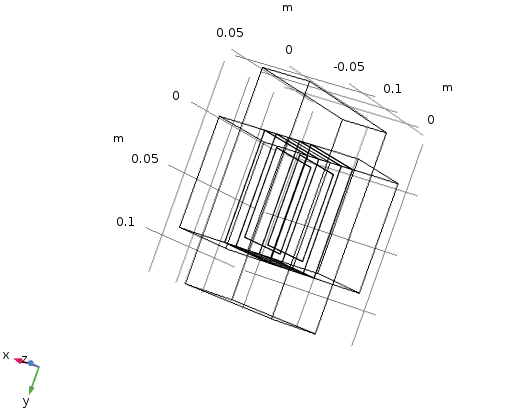
\includegraphics[width=0.4\textwidth]{attachments/fig.2.3.0.png}
		\caption{\textbf{The geometric model of the complex plate model}}
		\label{fig.2.3.0}
	\end{figure*}
	
	\begin{figure*}[htbp]
		\centering
		\subfloat[Temperature of the central face]{\label{fig.2.3.1}
		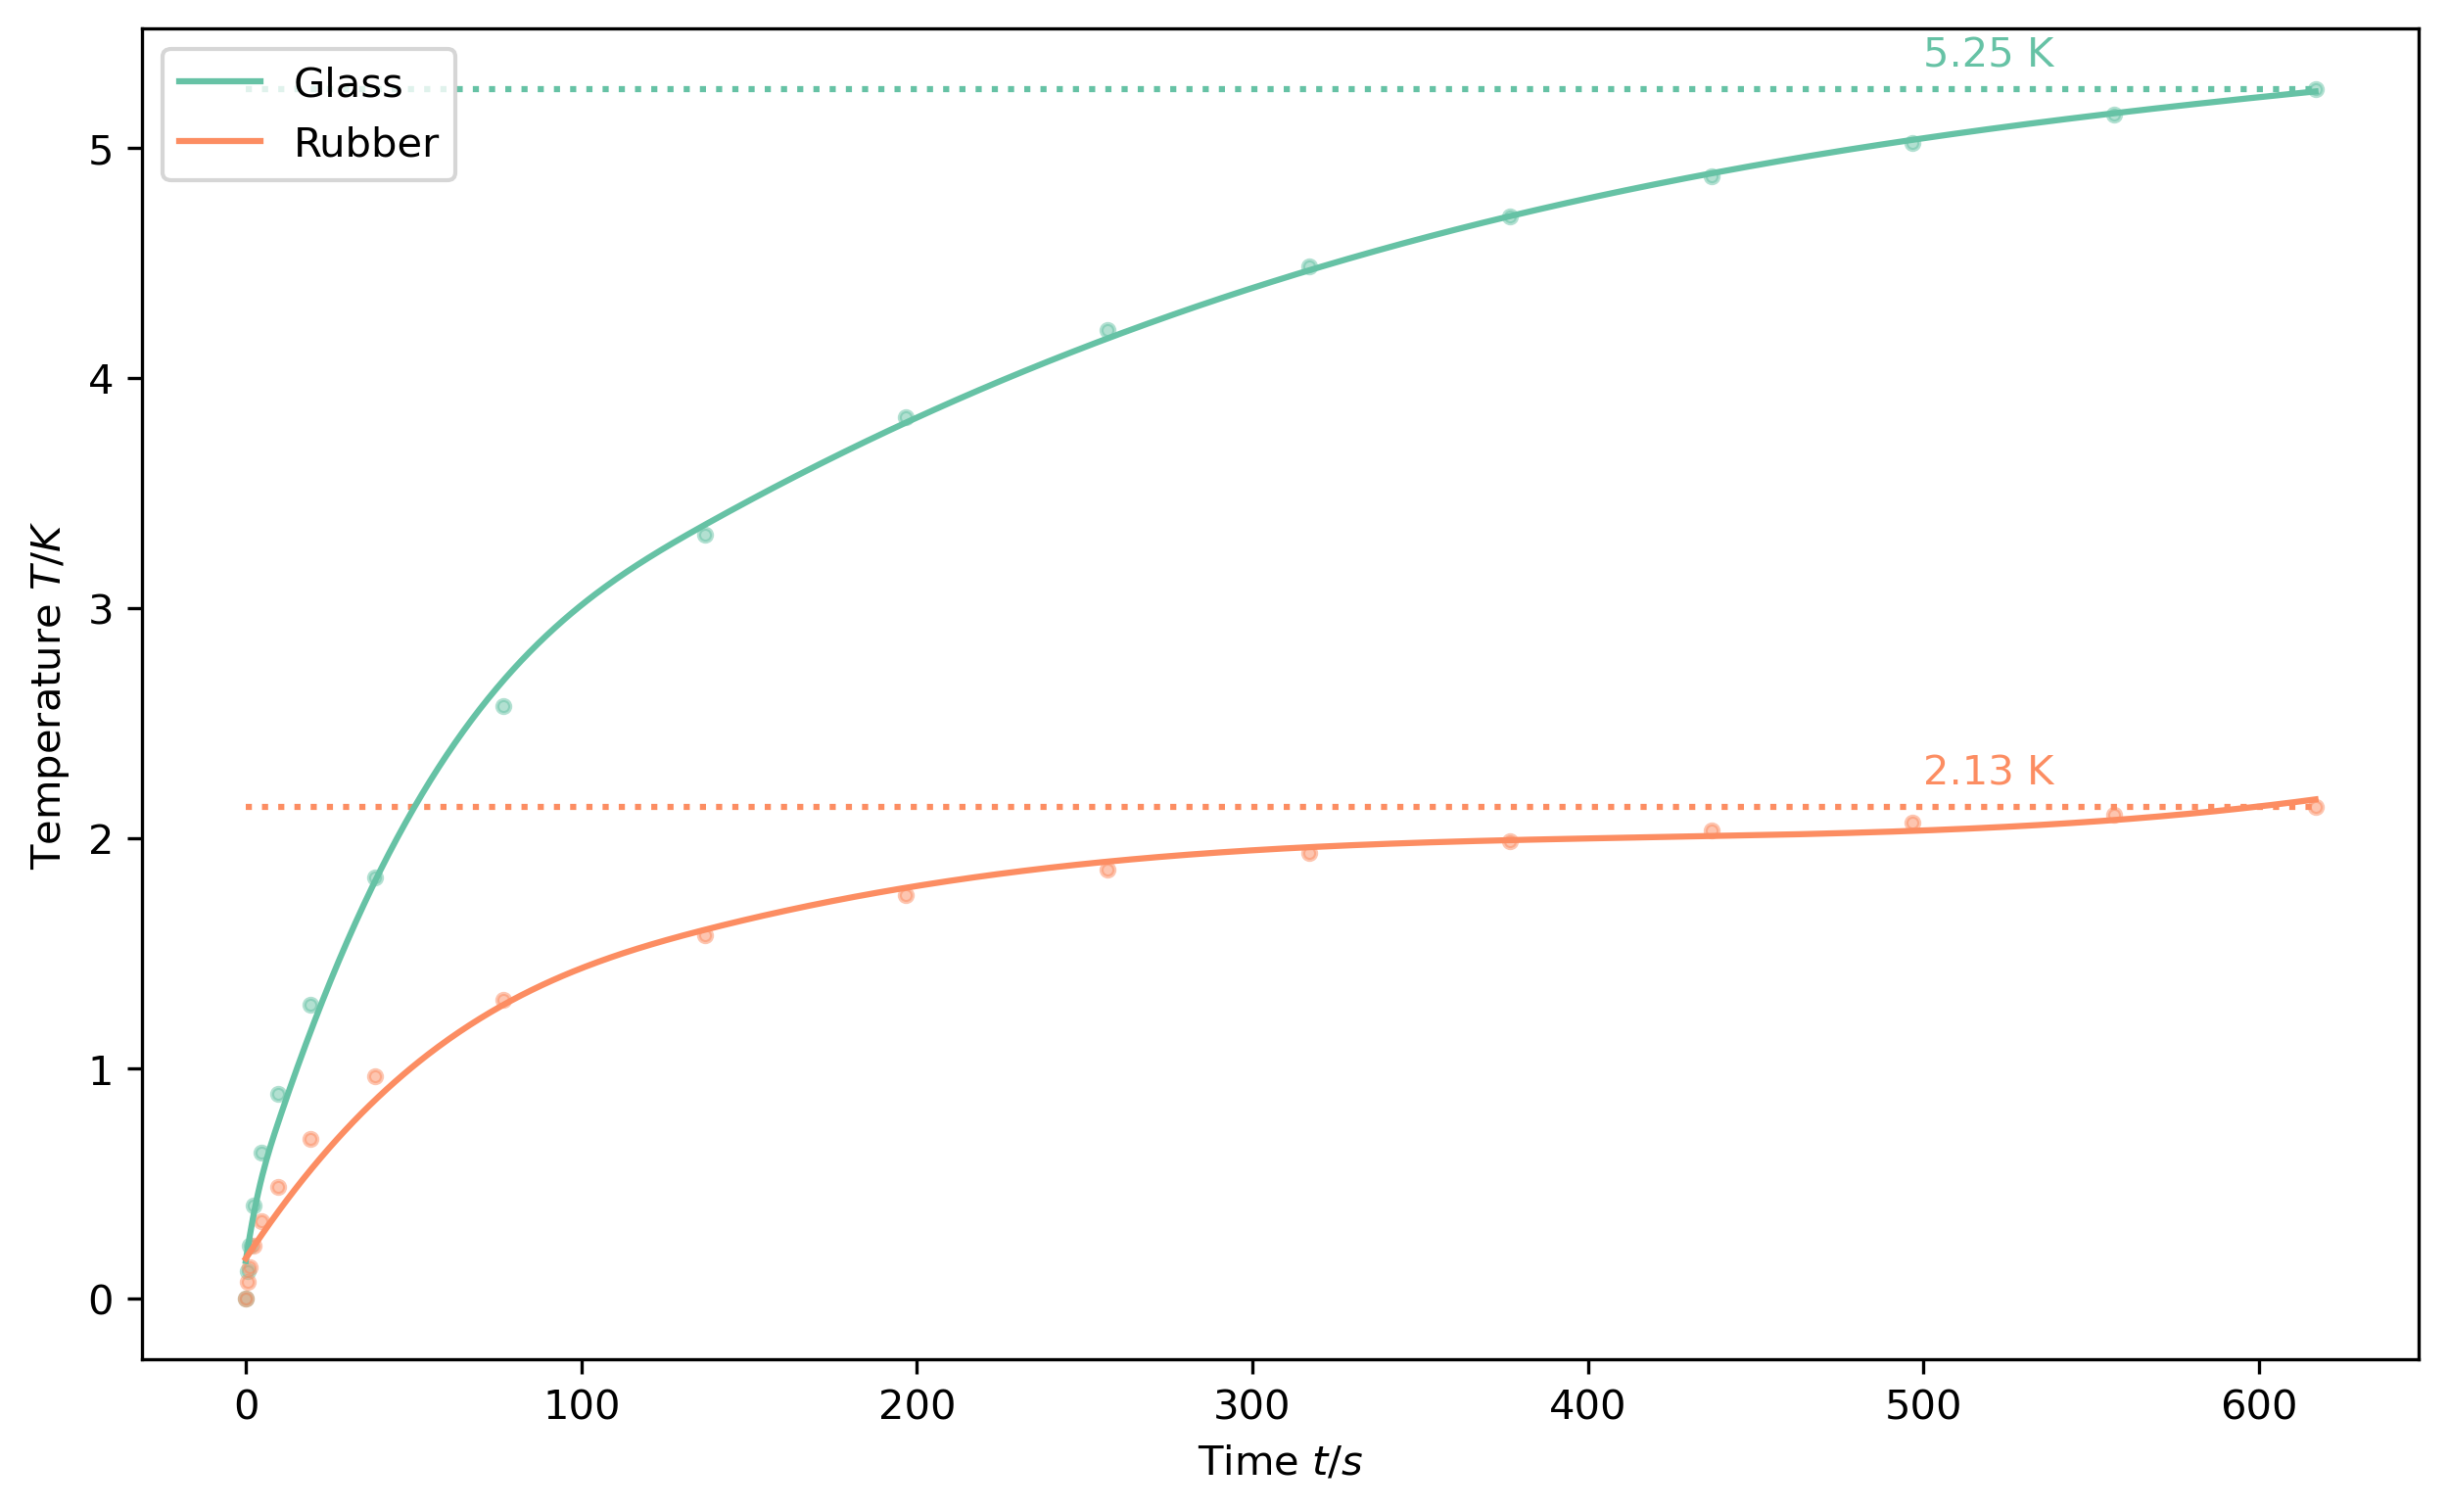
\includegraphics[width=0.4\textwidth]{attachments/fig.2.3.1.png}
		}		
		\subfloat[Temperature difference]{\label{fig.2.3.2}
		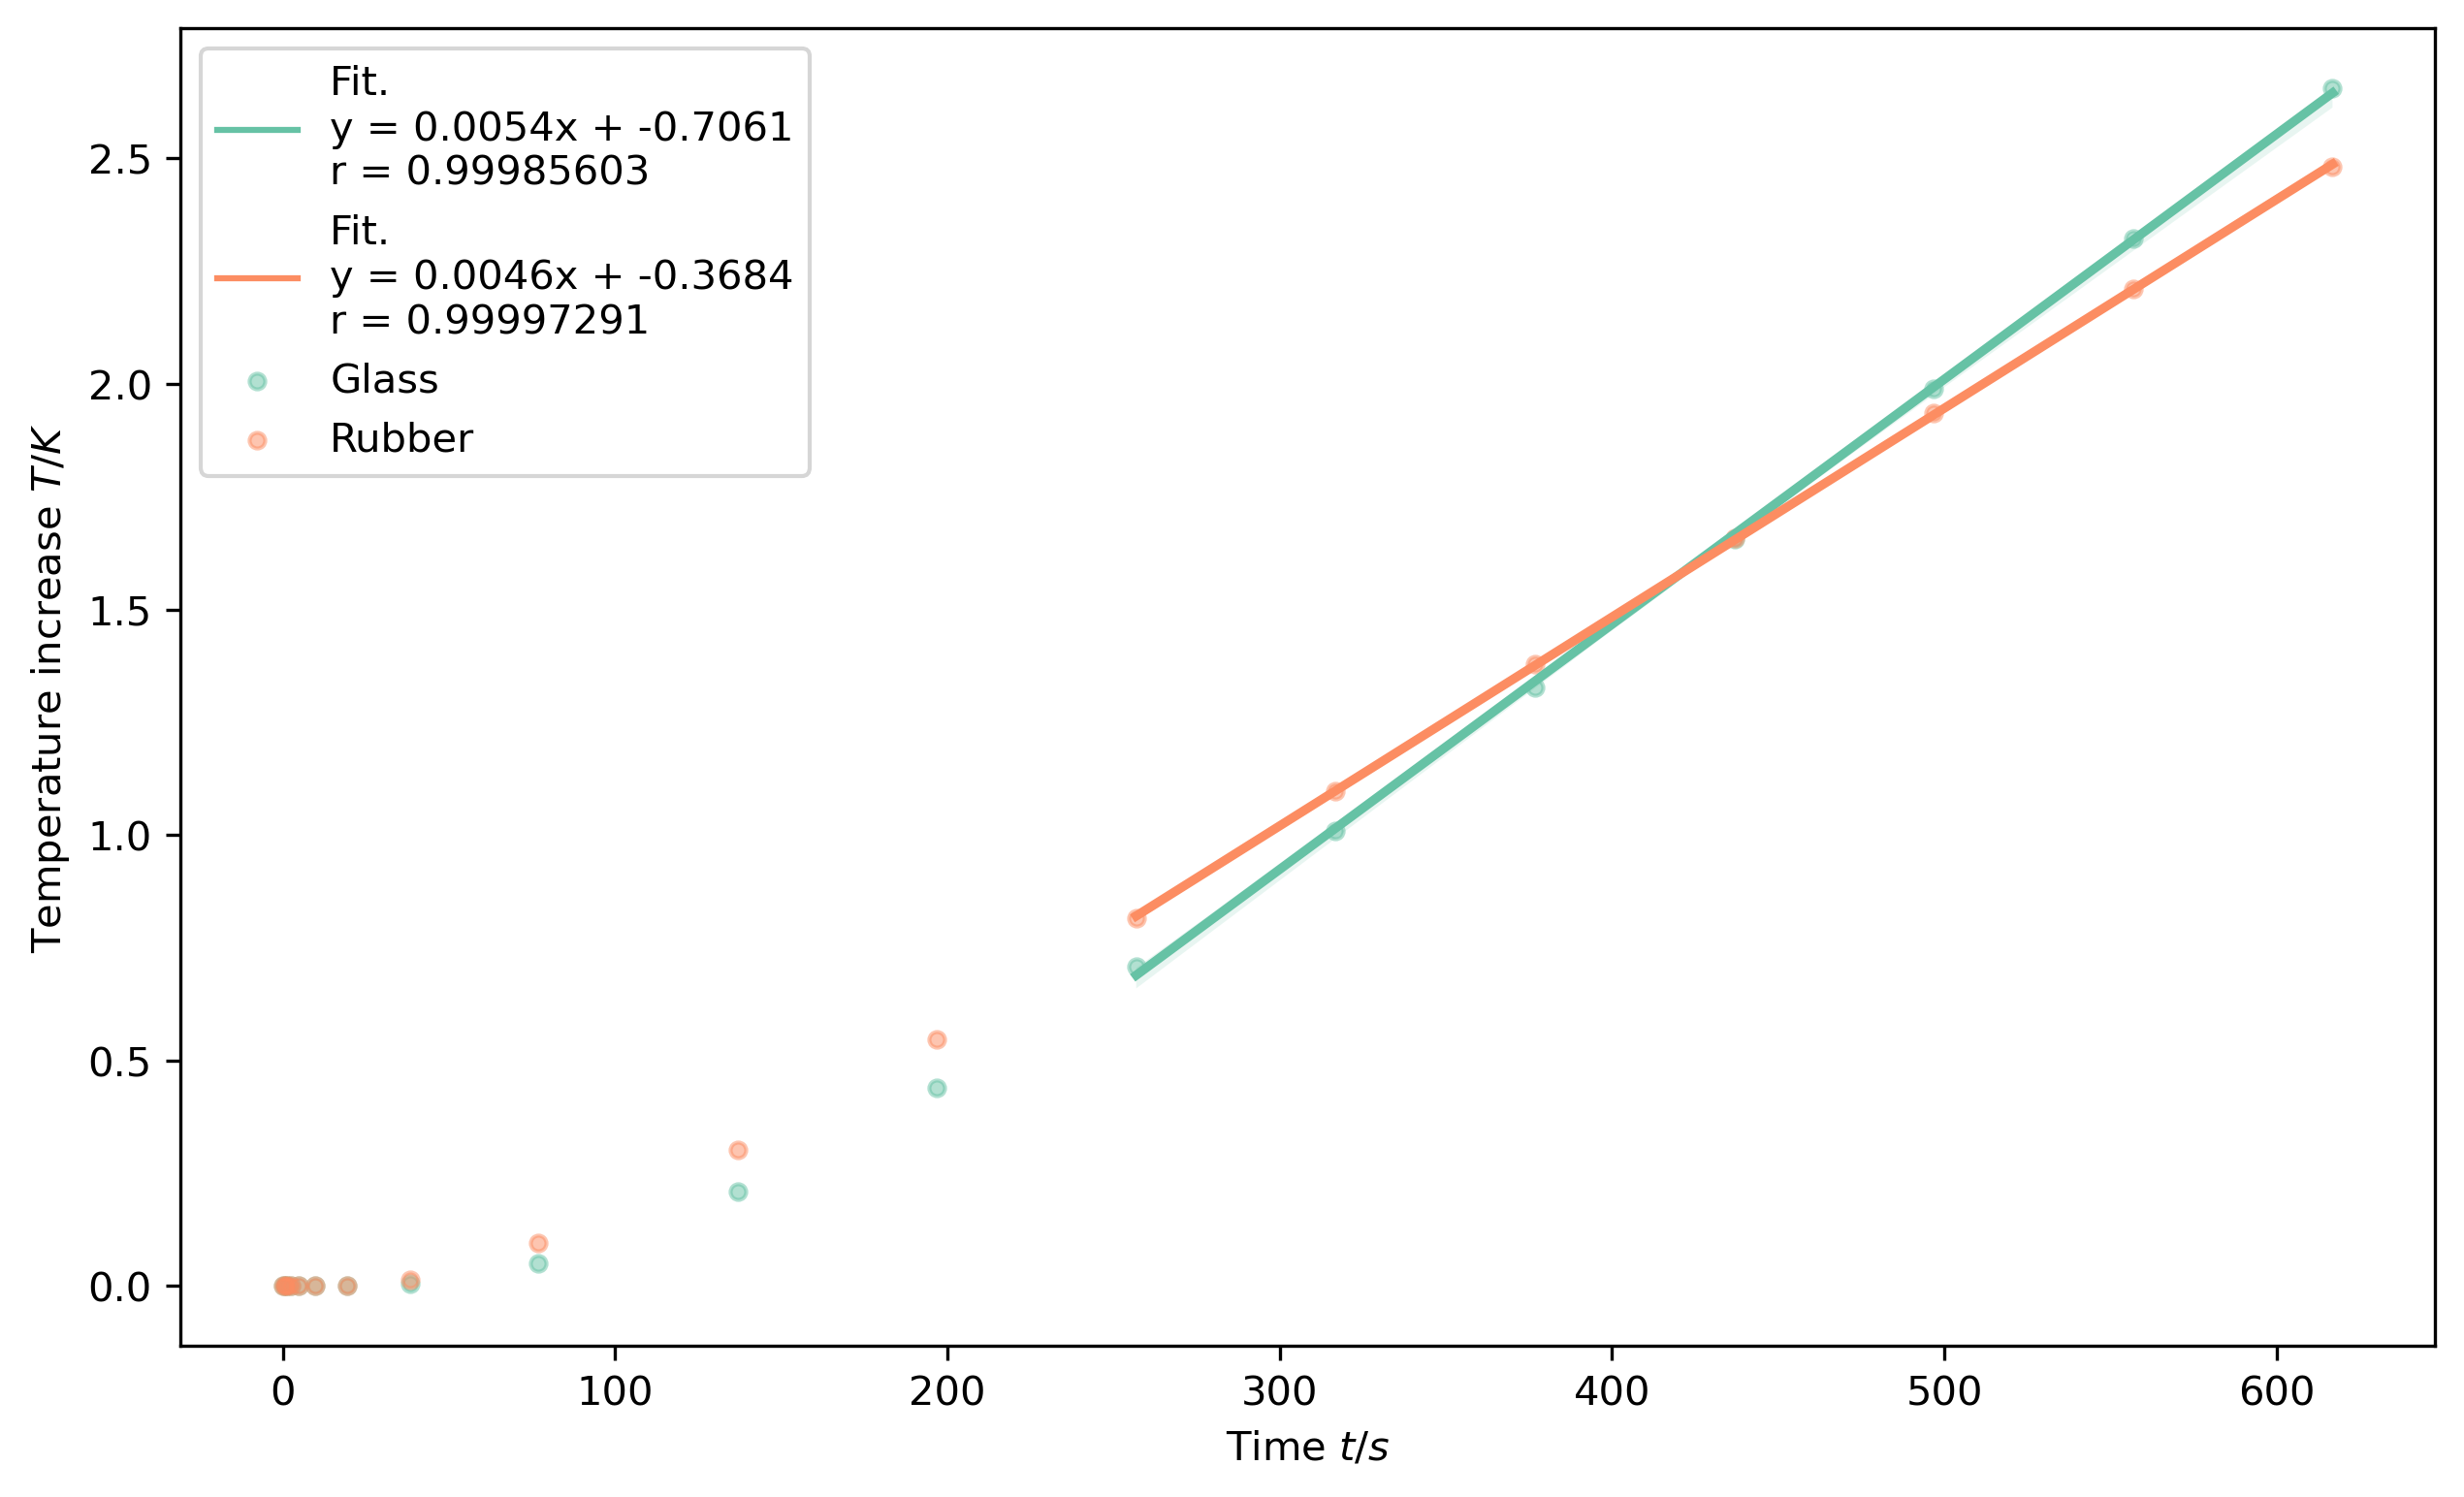
\includegraphics[width=0.4\textwidth]{attachments/fig.2.3.2.png}
		}
		\caption{\textbf{Thermal conduction of rubber or glass, simulation experiments of the complex model}}
		\label{fig.2.3}
	\end{figure*}


	\paragraph{C. Comparison of the three models}~
	The equilibrium temperature different between the central face and heating face and the changing rate of temperature at the quasi-stable state obtained from the three experiments are summarized in Tab. \ref{tab.2}.
	
	\begin{table*}[htbp]
	\centering
	\caption{\textbf{Summary of the equilibrium temperature difference and heating rate}}
	\label{tab.2}
		\begin{tabular}{ccccc}
			\toprule
			Sample & Par. & Real-world EXP. & Sim. Ideal mod. & Sim. Complex Mod. \\
			\midrule
			Organic glass & Heating rate $(K/s)$ & 0.0079 & 0.0091 & 0.0054 \\
			~ & Temperature difference $(K)$ & 4.13 & 4.56 & 5.25 \\
			Rubber & Heating rate $(K/s)$ & 0.0075 & 0.0065 & 0.0046 \\
			~ & Temperature difference $(K)$ & 1.85 & 1.80 & 2.13 \\
			\bottomrule
		\end{tabular}
	\end{table*}

	Still, out of our expectation, we found that the ideal model was even more accurate than the complex mode. 
	The final equilibrium temperature difference and the heating rate of the central face of the ideal model were all consistent with the real-world model, 
	while for the complex model, there is a great difference.
	Basing on the same hypothesis, that is, lack of necessary knowledge of the materials and the geomagnetic diameters will induce great uncertainty to the model,
	we admit that further improvement of the model is required.

	Anyway, the tendencies and general patterns of temperature changes are consistent among the three models, 
	which proves the effectiveness of these techniques in studying thermal conducting models with very complex boundary conditions.

%%end-------------------Result-----------------------%%

%%begin-------------------Conclusion and Discussion-----------------------%%
\section{Conclusion and Discussion}
	\subsection{Conclusion}
	In conclusion, in this research we conducted real-world temperature measurement basing on LabVIEW platform, and simulation experiments basing on COMSOL for both the resistor thermal model and the plate thermal model, 
	and revealed the characteristics of temperature fields of these models and their evolution over time. 
	Although the measurement values obtained from real-world experiments and simulation experiments were not exactly consistent, 
	the tendencies and general patterns of temperature changes are identical, which proves the effectiveness of these techniques in studying thermal conducting models with very complex boundary conditions.

	\subsection{Known limitation}
	As the complex model involved much more details, the precision of the values of the material properties and geometric dimensions becomes so essential that they have a dominant influence on the results.
	Due to lack of these necessary knowledge, however, the parameters were all set empirically in this research, which definitely will cause the results to be inaccurate.

	To further improve the performance of the model, it is critical to ascertain the accurate value of parameters involved in the model.


%%end-------------------Conclusion and Discussion-----------------------%%

%%begin--------------------Reference------------------------%%
\printbibliography[title=Reference] 
%%end--------------------Reference------------------------%%
\end{document}